% =============================================================
% Mémoire de Master — Modèle Oracle pour le downscaling climatique causalisé
% Fichier unifié combinant les chapitres I, II et III
% Style cible : gabarit Donald FEUZING NTEMMA (URIFIA 2024)
% =============================================================

\documentclass[14pt,a4paper,openany]{extreport}

% ---------- Encodage et langue ----------
\usepackage[T1]{fontenc}
\usepackage[utf8]{inputenc}
\usepackage[french]{babel}
\addto\captionsfrench{%
  \renewcommand{\tablename}{Tableau}%
  \renewcommand{\figurename}{Figure}%
}

\usepackage{lmodern}
\usepackage{setspace}
\onehalfspacing
\usepackage[a4paper,inner=3cm,outer=2.3cm,top=2.5cm,bottom=2.7cm,headheight=15pt,bindingoffset=0.3cm]{geometry}

\usepackage{amsmath,amssymb,amsthm}
\usepackage{graphicx}
\usepackage{xcolor}
\definecolor{uridarkblue}{RGB}{30,40,90}
\definecolor{urigray}{RGB}{70,70,70}
\definecolor{uriaccent}{RGB}{180,60,40}

\usepackage{array}
\usepackage{booktabs}
\usepackage{multirow}
\usepackage{tabularx}
\usepackage{longtable}

\usepackage{algorithm}
\usepackage{algpseudocode}

\usepackage[most]{tcolorbox}
\usepackage{tikz}
\usetikzlibrary{positioning, fit, shapes, arrows.meta, calc}

\renewcommand{\thechapter}{\Roman{chapter}}
\renewcommand{\thesection}{\thechapter.\arabic{section}}
\renewcommand{\thesubsection}{\thesection.\arabic{subsection}}
\renewcommand{\thesubsubsection}{\thesubsection.\arabic{subsubsection}}

\makeatletter
\renewcommand{\@makechapterhead}[1]{%
  \vspace*{20\p@}%
  {\parindent \z@ \centering \normalfont
    \textsc{\large Chapitre}\par
    \vspace{0.3em}
    {\color{uridarkblue}\fontsize{60}{72}\selectfont\bfseries\thechapter\par}
    \vspace{1em}
    {\color{uridarkblue}\Large\bfseries\MakeUppercase{#1}\par}
    \vspace{1em}
    \rule{0.4\linewidth}{0.6pt}\par
    \vspace{2em}
  }}
\renewcommand{\@makeschapterhead}[1]{%
  \vspace*{20\p@}%
  {\parindent \z@ \centering \normalfont
    {\color{uridarkblue}\Large\bfseries\MakeUppercase{#1}\par}
    \vspace{1em}
    \rule{0.4\linewidth}{0.6pt}\par
    \vspace{2em}
  }}
\makeatother

\usepackage{titlesec}
\titleformat{\section}
  {\normalfont\Large\bfseries\color{uridarkblue}}
  {\thesection.}{0.8em}{}
\titleformat{\subsection}
  {\normalfont\large\bfseries}
  {\thesubsection.}{0.7em}{}
\titleformat{\subsubsection}
  {\normalfont\normalsize\bfseries\itshape}
  {\thesubsubsection.}{0.6em}{}

\usepackage{fancyhdr}
\pagestyle{fancy}
\fancyhf{}
\fancyhead[L]{\textsc{\nouppercase{\leftmark}}}
\fancyhead[R]{\thepage}
\fancyfoot[L]{\footnotesize Mémoire de Master en Informatique, Université de Dschang}
\fancyfoot[R]{\footnotesize URIFIA}
\renewcommand{\headrulewidth}{0.4pt}
\renewcommand{\footrulewidth}{0.2pt}
\renewcommand{\chaptermark}[1]{\markboth{#1}{}}
\renewcommand{\sectionmark}[1]{\markright{\thesection\ #1}{}}

\usepackage[font=small,labelfont={sc,bf},textfont=it]{caption}
\renewcommand{\thefigure}{\arabic{figure}}
\renewcommand{\thetable}{\arabic{table}}

\usepackage[numbers,square,sort&compress]{natbib}
\usepackage[hidelinks]{hyperref}

\theoremstyle{definition}
\newtheorem{definition}{Définition}[chapter]
\newtheorem{propriete}[definition]{Propriété}
\newtheorem{remarque}[definition]{Remarque}

\newcommand{\Oracle}{\textsc{Oracle}}
\newcommand{\CorrDiff}{\textsc{CorrDiff}}
\newcommand{\LR}{\ensuremath{\text{LR}}}
\newcommand{\HR}{\ensuremath{\text{HR}}}
\newcommand{\xHR}{\ensuremath{x_{\HR}}}
\newcommand{\yLR}{\ensuremath{y_{\LR}}}
\newcommand{\muHR}{\ensuremath{\mu_{\HR}}}
\newcommand{\Adag}{\ensuremath{A_{\mathrm{dag}}}}
\newcommand{\Ht}{\ensuremath{H_t}}
\newcommand{\HT}{\ensuremath{H_T}}
\newcommand{\Lmse}{\ensuremath{\mathcal{L}_{\mathrm{mse}}}}
\newcommand{\Lrec}{\ensuremath{\mathcal{L}_{\mathrm{rec}}}}
\newcommand{\LDAGMA}{\ensuremath{\mathcal{L}_{\mathrm{DAGMA}}}}
\newcommand{\LLone}{\ensuremath{\mathcal{L}_{L_1}}}
\newcommand{\LEDM}{\ensuremath{\mathcal{L}_{\mathrm{EDM}}}}
\newcommand{\Ltotal}{\ensuremath{\mathcal{L}_{\mathrm{total}}}}

\newtcolorbox{sommairebox}{
  enhanced,colback=white,colframe=urigray,boxrule=0.5pt,arc=0pt,
  left=1.5em,right=1.5em,top=0.8em,bottom=0.8em,
  title={\textsc{Sommaire}},
  attach boxed title to top center={yshift=-2mm,xshift=0mm},
  boxed title style={colback=white,colframe=white,coltitle=urigray,boxrule=0pt,
    left=0.8em,right=0.8em,top=0pt,bottom=0pt},
  fonttitle=\bfseries\small,
}

\newtcolorbox{disclaimerbox}{
  enhanced,colback=uriaccent!4,colframe=uriaccent!60,boxrule=0.7pt,arc=2pt,
  left=1em,right=1em,top=0.6em,bottom=0.6em,
  title={\textsc{Portée et limites}},
  attach boxed title to top left={yshift=-2mm,xshift=10pt},
  boxed title style={colback=uriaccent!10,colframe=uriaccent!60,boxrule=0.5pt,
    arc=2pt,left=0.6em,right=0.6em,top=0pt,bottom=0pt},
  fonttitle=\bfseries\small\color{uriaccent},
}

\newcommand{\figplaceholder}[2][0.9\linewidth]{%
  \begin{tcolorbox}[width=#1,height=5cm,valign=center,colback=gray!8,colframe=gray!45,arc=2pt,boxrule=0.5pt]
    \centering\small\textit{#2}
  \end{tcolorbox}%
}

\providecommand{\chaplabel}[1]{}

\begin{document}

% Pages preliminaires en chiffres romains
\pagenumbering{roman}

% =============================================================
% PAGE DE GARDE
% =============================================================
\thispagestyle{empty}
\begin{titlepage}
\centering

% --- Bandeau supérieur ---
{\large \textsc{République du Cameroun} \par}
\vspace{0.2em}
{\small \textit{Paix -- Travail -- Patrie} \par}
\vspace{0.5em}
{\large \textsc{Ministère de l'Enseignement Supérieur} \par}
\vspace{0.5em}
{\large \textbf{Université de Dschang} \par}
\vspace{0.3em}
{\large \textit{Faculté des Sciences} \par}
\vspace{0.3em}
{\large \textit{Unité de Recherche d'Informatique Fondamentale et Appliquée (URIFIA)} \par}

\vspace{2em}
% --- Logo placeholder ---
\begin{tcolorbox}[width=4cm,height=4cm,valign=center,colback=gray!10,colframe=gray!50,arc=2pt]
\centering\small\textit{Logo UD}
\end{tcolorbox}

\vspace{2em}
% --- Type de document ---
{\Large \textsc{Mémoire de Master en Informatique} \par}
\vspace{0.5em}
{\large \textit{Option : Intelligence Artificielle et Sciences des Données} \par}

\vspace{2.5em}
% --- Titre principal ---
\begin{tcolorbox}[colback=uridarkblue!5,colframe=uridarkblue,boxrule=1pt,arc=2pt,
                  left=0.5em,right=0.5em,top=0.8em,bottom=0.8em]
\centering
{\LARGE\bfseries\color{uridarkblue}
ORACLE : une architecture causale à deux étages\\pour le downscaling climatique probabiliste \par}
\vspace{0.8em}
{\large\itshape Application à la précipitation haute résolution\\sous changement climatique \par}
\vspace{0.8em}
{\normalsize\itshape Une architecture conditionnelle structurée pour le downscaling probabiliste des précipitations : entre causalité architecturale et identification physique. \par}
\end{tcolorbox}

\vspace{2.5em}
% --- Auteur ---
{\large \textit{Présenté et soutenu publiquement par :} \par}
\vspace{0.5em}
{\Large\bfseries Leonel KENFACK \par}
\vspace{0.2em}
{\normalsize \textit{en vue de l'obtention du diplôme de Master en Informatique} \par}

\vspace{2em}
% --- Jury ---
{\large \textit{Sous la direction de :} \par}
\vspace{0.4em}
{\large \textsc{Pr.~[Nom du directeur]} \par}
{\small \textit{[Titre, affiliation, Université de Dschang]} \par}

\vspace{1.5em}
% --- Date ---
{\large \textbf{Année académique 2025--2026} \par}

\end{titlepage}

% =============================================================
% DÉDICACE
% =============================================================
\clearpage
\thispagestyle{empty}
\vspace*{4cm}
\begin{flushright}
\textit{À mes parents,}\\[0.5em]
\textit{dont la patience et le soutien constant ont rendu possible}\\[0.3em]
\textit{ce parcours d'études supérieures.}\\[1em]
\textit{À celles et ceux qui, en Afrique centrale comme ailleurs,}\\[0.3em]
\textit{cherchent des outils pour comprendre et anticiper}\\[0.3em]
\textit{le climat de leur quotidien.}\\[2em]
\end{flushright}

% =============================================================
% REMERCIEMENTS
% =============================================================
\clearpage
\chapter*{Remerciements}
\addcontentsline{toc}{chapter}{Remerciements}
\markboth{Remerciements}{Remerciements}

Ce mémoire n'aurait pu être mené sans l'apport et le soutien de plusieurs personnes et structures que je tiens à remercier.

Je remercie mon directeur de mémoire, le \textbf{Pr.~[Nom à compléter]}, pour sa disponibilité, la rigueur de ses relectures et la confiance qu'il m'a accordée. Ses conseils méthodologiques, en particulier sur la nécessité d'expliciter les variantes écartées, ont structuré la forme finale du manuscrit. Je remercie les membres du jury qui ont accepté d'évaluer ce travail.

Je remercie l'\textbf{Unité de Recherche d'Informatique Fondamentale et Appliquée (URIFIA)} de l'Université de Dschang pour le cadre scientifique offert pendant les deux années de master, ainsi que les contributeurs des projets logiciels open-source --- \textsc{PyTorch}, \textsc{PyTorch~Geometric}, l'implémentation \textsc{NVIDIA~PhysicsNeMo} de \textsc{CorrDiff} --- et les jeux de données mis à disposition par les contributeurs au \emph{Coupled Model Intercomparison Project} (CMIP6).

Je remercie enfin ma famille et mes proches, dont le soutien quotidien a rendu ces deux années fertiles.

% =============================================================
% RÉSUMÉ + ABSTRACT (sur une seule page)
% =============================================================
\clearpage
\thispagestyle{plain}
\addcontentsline{toc}{chapter}{Résumé / Abstract}
\markboth{Résumé / Abstract}{Résumé / Abstract}

\begingroup
\small
\setlength{\parskip}{0.3em}

\begin{center}{\large\bfseries\color{uridarkblue}Résumé}\end{center}

Le \emph{downscaling} climatique transforme des champs atmosphériques basse résolution issus de modèles globaux en champs haute résolution exploitables localement. Les architectures profondes récentes (cGAN résiduels, diffusion à deux étages) améliorent qualité prédictive et calibration mais restent fragiles sous changement de distribution. Ce mémoire propose \Oracle{}, une architecture à deux étages qui place la causalité dans la topologie du graphe de calcul : un encodeur intelligible par variable, un graphe hétérogène à six nœuds, un réseau causal récurrent gouverné par une matrice apprise sous contrainte DAGMA et un décodeur graphe-à-grille produisent une moyenne haute résolution ; une diffusion EDM résiduelle conditionnée par concaténation de canaux échantillonne le résidu, garantissant par construction la propriété d'indispensabilité du DAG~(O3).

Sur la Nouvelle-Zélande (ACCESS-CM2 en distribution ; EC-Earth3, NorESM2-MM hors-distribution), \Oracle{} réduit le CRPS de $40\%$ en ID et de $30\%$ en inter-GCM historique. Le ratio \emph{spread-skill} passe de $0{,}20$ à $0{,}69$ ($\times 3{,}5$) ; la distance spectrale chute d'un facteur $450$. La réponse à deux perturbations contrôlées ($\Delta q+20\%$, $\Delta t+3$~K) coïncide avec le signe physique attendu, là où la baseline non-causale échoue sur l'intervention thermique. Le mémoire assume ses limites : le DAG appris reste à magnitudes plates ($Q_{\mathrm{phys}}=0{,}40$), à lire comme une régularisation structurelle inductive plutôt qu'une cartographie causale identifiée.

\noindent\textbf{Mots-clés :} downscaling climatique, modèles de diffusion, EDM, causalité architecturale, DAGMA, robustesse inter-GCM en régime historique, précipitation, CMIP6, intervention contrôlée, calibration d'ensemble.

\vspace{0.6em}\hrule\vspace{0.6em}

\begin{center}{\large\bfseries\color{uridarkblue}Abstract}\end{center}

Climate downscaling transforms low-resolution atmospheric fields from global climate models into high-resolution fields suitable for local decision-making. Recent deep architectures (residual cGANs, two-stage diffusion) improve predictive accuracy and probabilistic calibration but remain fragile under distribution shift. This thesis proposes \textsc{Oracle}, a two-stage architecture that places causality in the computation graph topology: a per-variable intelligible encoder, a six-node heterogeneous graph, a recurrent causal network governed by a DAGMA-constrained learned matrix and a graph-to-grid decoder produce a high-resolution mean; a residual EDM diffusion conditioned by channel concatenation samples the residual, guaranteeing by construction the DAG indispensability property (O3).

Over New Zealand (ACCESS-CM2 in-distribution; EC-Earth3, NorESM2-MM out-of-distribution), \textsc{Oracle} reduces the CRPS by $40\%$ in-distribution and by $30\%$ inter-GCM. The spread-skill ratio rises from $0.20$ to $0.69$ ($\times 3.5$); the spectral distance drops by a factor of $450$. The response to two controlled perturbations ($\Delta q+20\%$, $\Delta t+3$~K) matches the expected physical sign, whereas the non-causal baseline fails on the thermal intervention. The thesis openly assumes its limitations: the learned DAG remains with flat magnitudes ($Q_{\mathrm{phys}}=0.40$), to be read as inductive structural regularisation rather than identified causal mapping.

\noindent\textbf{Keywords:} climate downscaling, diffusion models, EDM, architectural causality, DAGMA, inter-GCM robustness in historical regime, precipitation, CMIP6, controlled intervention, ensemble calibration.

\endgroup

% =============================================================
% LISTE DES ABRÉVIATIONS ET SIGLES
% =============================================================
\clearpage
\chapter*{Liste des abréviations et sigles}
\addcontentsline{toc}{chapter}{Liste des abréviations et sigles}
\markboth{Liste des abréviations et sigles}{Liste des abréviations et sigles}

\begin{longtable}{p{3cm} p{11.5cm}}
\toprule
\textbf{Sigle} & \textbf{Signification} \\
\midrule
\endhead

ACCESS-CM2 & GCM australien utilisé en distribution (CMIP6) \\
CASTLE & \emph{Causal Structure Learning via Auxiliary Causal Graph Discovery} (Kyono~2020) \\
CC & Clausius-Clapeyron, relation vapeur saturante / température \\
CDD & \emph{Consecutive Dry Days}, jours secs consécutifs (ETCCDI) \\
cGAN & \emph{Conditional Generative Adversarial Network} \\
CMIP6 & \emph{Coupled Model Intercomparison Project Phase 6} \\
\CorrDiff{} & Architecture two-stage de diffusion résiduelle (Mardani~2024) \\
CRPS / CRPS-SS & \emph{Continuous Ranked Probability Score} et son skill score \\
DAG & \emph{Directed Acyclic Graph}, graphe acyclique dirigé \\
DAGMA & \emph{DAG via M-matrices and log-determinant Acyclicity} (Bello~2022) \\
DDPM / EDM & \emph{Denoising Diffusion Probabilistic Models} (Ho~2020) / EDM (Karras~2022) \\
EC-Earth3, NorESM2-MM & GCM utilisés en hors-distribution \\
ERA5 & Réanalyse atmosphérique de référence (Hersbach~2020) \\
ETCCDI & \emph{Expert Team on Climate Change Detection and Indices} \\
F1@p95/p99 & Score F1 sur les pixels excédant le quantile p95 ou p99 \\
FNO / FSS & \emph{Fourier Neural Operator} / \emph{Fractions Skill Score} \\
GAN & \emph{Generative Adversarial Network} \\
GCM / RCM & Modèle de circulation générale / modèle climatique régional \\
GIEC / IPCC & Groupe d'experts intergouvernemental sur l'évolution du climat \\
GP & Géopotentiel, à différents niveaux de pression (GP850, GP500, GP250) \\
GRU & \emph{Gated Recurrent Unit} (Cho~2014) \\
HR / LR & Haute / basse résolution \\
ID / OOD & En distribution / hors-distribution \\
IG & \emph{Integrated Gradients} (Sundararajan~2017) \\
MAE / MSE / RMSE & Erreurs ponctuelles standards \\
$Q_{\mathrm{int}}$, $Q_{\mathrm{phys}}$ & Score interventionnel / orientation physique du DAG \\
RAPSD / PSD & \emph{Power Spectral Density} radialement moyennée \\
RCN & \emph{Recurrent Causal Network}, réseau causal récurrent \\
R10mm / RX1day / CDD & Indices ETCCDI sur la précipitation \\
SCM & \emph{Structural Causal Model} (Pearl) \\
SSP & \emph{Shared Socioeconomic Pathway}, scénario CMIP6 \\
UNet & Architecture U pour segmentation et diffusion (Ronneberger~2015) \\
URIFIA & Unité de Recherche d'Informatique Fondamentale et Appliquée \\
\bottomrule
\end{longtable}

\cleardoublepage
\tableofcontents
\cleardoublepage


% Corps du memoire en chiffres arabes
\pagenumbering{arabic}
\setcounter{page}{1}

\chapter*{Introduction générale}
\addcontentsline{toc}{chapter}{Introduction générale}
\markboth{Introduction générale}{Introduction générale}

Nous proposons une architecture de downscaling probabiliste dans laquelle un graphe structurel appris régularise un modèle de diffusion conditionnel. Nous n'identifions pas un effet causal au sens de Pearl ; nous mesurons une cohérence interventionnelle architecturale et nous en cartographions empiriquement les limites.

\section*{Contexte et motivation}

Le changement climatique impose des décisions à des échelles spatiales que les modèles climatiques globaux contributeurs au projet CMIP6~\cite{eyring_cmip6_2016} ne fournissent pas immédiatement. Ces modèles simulent l'atmosphère à une résolution de l'ordre de la centaine de kilomètres, suffisante pour les grands modes de variabilité, mais très en deçà de ce qu'exige la planification locale d'infrastructures, l'agriculture pluviale ou la gestion du risque hydrologique. La précipitation présente une structure spatiale qui se déploie sur quelques kilomètres et qui interagit fortement avec le relief : un modèle qui produit une valeur moyenne sur cent kilomètres ne peut pas restituer cette structure. C'est cet écart d'échelle que cherche à combler le \emph{downscaling} climatique.

La motivation finale est l'aide à la décision dans des régions à forte vulnérabilité hydrologique et faible densité d'observations, dont l'Afrique subsaharienne. \textbf{Le présent mémoire n'apporte cependant aucune preuve directe de transférabilité géographique.} Nous traitons la Nouvelle-Zélande comme un terrain expérimental rigoureux --- orographie marquée, densité d'observations élevée --- pour isoler proprement l'effet de la causalisation. Toute extension à l'Afrique reste hypothétique au stade actuel et est portée comme axe 5 de perspectives. Les outils existants ne fournissent pas ce service de manière satisfaisante : ils sont soit déterministes (donc impropres au raisonnement sur le risque), soit insuffisamment résolus, soit non transférables hors de leur domaine de calibration~\cite{maraun_widmann_2018}.

\section*{Problématique}

Les architectures profondes récentes pour le downscaling --- réseaux antagonistes génératifs résiduels, modèles de diffusion à deux étages --- ont amélioré la qualité prédictive et la calibration probabiliste. Elles restent toutefois fragiles sous changement de distribution : un modèle entraîné sur le climat historique apprend des associations contingentes au régime d'entraînement, qu'aucune régularisation a posteriori ne garantit de redresser. La causalité structurelle est, en théorie, une réponse de principe à cette fragilité --- un modèle organisé autour de relations causales identifiées devrait mieux transférer en inter-GCM historique. Mais cette promesse n'a pas été opérationnalisée dans un downscaler génératif probabiliste qui aille au-delà du diagnostic post-hoc.

Le paysage actuel peut être résumé par un trilemme : aucune approche existante ne garantit simultanément la stabilité d'entraînement, le réalisme des extrêmes et la robustesse inter-GCM en régime historique. Le paradigme \emph{two-stage} de Mardani et~al.~\cite{mardani_corrdiff_2023}, qui combine un prédicteur de moyenne déterministe et un décodeur de diffusion résiduelle, constitue à ce jour la réponse la plus crédible aux deux premières propriétés mais n'adresse pas la troisième : son premier étage n'est qu'un réseau de régression générique, aussi vulnérable au changement de climat qu'un modèle monolithique. La question centrale de ce mémoire est donc : \emph{est-il possible de causaliser le premier étage du paradigme two-stage de manière à doter le downscaling probabiliste d'une robustesse de principe sous changement climatique, sans dégrader la stabilité ni le réalisme acquis} ?

\section*{Questions de recherche, objectifs et hypothèses}

Trois questions structurent la suite. \textbf{Q1.} Les architectures génératives existantes (cGAN résiduel, \CorrDiff{}) suffisent-elles à garantir une robustesse inter-GCM en régime historique ? \textbf{Q2.} Un modèle causal structurel intégré dans une dynamique récurrente permet-il de mieux guider le downscaling probabiliste, et selon quelle interface avec un décodeur de diffusion résiduelle ? \textbf{Q3.} Quelles métriques permettent de discriminer une véritable causalité architecturale d'une simple structuration corrélationnelle ?

La conception du modèle obéit à six objectifs notés O1 à O6, repris au chapitre III : \textbf{O1} stabilité d'entraînement, \textbf{O2} réalisme des extrêmes, \textbf{O3} causalité architecturale (la matrice $\Adag$ doit être indispensable à la prédiction par construction), \textbf{O4} robustesse inter-GCM en régime historique, \textbf{O5} efficacité computationnelle, \textbf{O6} interprétabilité.

Trois hypothèses de travail sont formulées en début de projet. \textbf{H1.} Un modèle apprenant des relations structurelles sous contrainte d'acyclicité, dans une dynamique récurrente, généralise mieux qu'un modèle purement corrélatif. \textbf{H2.} La séparation entre moyenne causale déterministe et résidu stochastique stabilise l'entraînement et améliore la calibration. \textbf{H3.} L'indispensabilité architecturale du DAG limite le risque qu'il ne soit qu'un décor inopérant, sans pour autant garantir une identification causale au sens strict.

\noindent\textbf{Précision terminologique.} L'expression « causalité architecturale » désigne une \emph{régularisation structurelle inductive} : la matrice $\Adag$ est indispensable au chemin de calcul (ablation $\Rightarrow$ chute de performance), ce qui prouve une dépendance fonctionnelle, non une identification causale au sens de Pearl~\cite{pearl_causality_2009}. La contrainte d'acyclicité DAGMA est un dispositif de traitabilité ; la physique atmosphérique réelle comporte des boucles de rétroaction qu'un graphe acyclique n'encode pas. Le DAG appris doit donc être lu comme un \emph{graphe de contraintes fonctionnelles}.

\textbf{Évaluation prévue des hypothèses.} H1 (causalité $\to$ robustesse inter-GCM) sera évaluée par comparaison CRPS et signes interventionnels. H2 (moyenne déterministe + résidu stochastique $\to$ stabilité + calibration) par les ratios spread/skill et la convergence d'entraînement. H3 (O3 architectural $\to$ pas de DAG décoratif) par l'ablation de la matrice apprise. Le bilan détaillé figure en conclusion.

\section*{Contributions et organisation}

Le mémoire propose quatre contributions. \textbf{C1.} Une architecture \emph{two-stage} causale, \Oracle{}, qui place la causalité architecturale dans un chemin de calcul indispensable plutôt que dans une régularisation de la perte. \textbf{C2.} Un réseau causal récurrent (RCN) intégrant dans une seule cellule un modèle causal structurel dynamique, une mise à jour récurrente GRU et une pénalité d'acyclicité DAGMA~\cite{bello_dagma_2022}. \textbf{C3.} Une interface inter-étages par concaténation de canaux, qui garantit qu'aucune information ne contourne le chemin causal. \textbf{C4.} Un protocole expérimental centré sur la calibration probabiliste, les extrêmes et les ablations causales --- incluant un test d'intervention $Q_{\mathrm{int}}$ sur des variables atmosphériques, original dans le contexte du downscaling profond.

Le manuscrit est organisé en quatre chapitres suivis d'une conclusion. Le \textbf{chapitre I} pose les fondements du downscaling climatique probabiliste et introduit le trilemme. Le \textbf{chapitre II} examine l'état de l'art par familles (déterministes, génératifs adversariaux, à vraisemblance, diffusion) et identifie le \emph{gap} scientifique qui motive la contribution. Le \textbf{chapitre III} présente formellement \Oracle{} : graphe atmosphérique hétérogène, encodeur intelligible, RCN, apprentissage du DAG sous contrainte DAGMA, décodeur graphe-à-grille, interface inter-étages, étage 2 de diffusion résiduelle EDM. Le \textbf{chapitre IV} décrit les matériels, méthodes, expérimentations et discussion : environnement, données, topologie effective d'\\Oracle{}, trajectoire de développement, protocole d'évaluation, résultats observés et discussion critique. La \textbf{conclusion générale} reprend les contributions, répond aux questions de recherche, identifie les limites et propose des perspectives.

\cleardoublepage


% ============= CHAPITRE I =============

\chapter{Fondements du downscaling climatique}
\label{chap:fondements}

% ---------- Boîte SOMMAIRE manuelle ----------
\begin{sommairebox}
\small
\noindent I.1 \ Introduction \dotfill \pageref{sec:intro}\\
\noindent I.2 \ Contexte climatique et besoin de désagrégation \dotfill \pageref{sec:contexte}\\
\noindent I.3 \ Données climatiques et leurs propriétés \dotfill \pageref{sec:donnees}\\
\noindent I.4 \ Approches classiques de downscaling \dotfill \pageref{sec:classiques}\\
\noindent I.5 \ Approches probabilistes et génératives \dotfill \pageref{sec:generatifs}\\
\noindent I.6 \ Causalité et modèles structurels \dotfill \pageref{sec:causalite}\\
\noindent I.7 \ Verrous scientifiques et trilemme \dotfill \pageref{sec:verrous}\\
\noindent I.8 \ Synthèse \dotfill \pageref{sec:synthese}
\end{sommairebox}

\vspace{1.5em}

% =============================================================
\section{Introduction}
\label{sec:intro}
% =============================================================

L'intensification du changement climatique et la fréquence croissante d'événements extrêmes imposent aux communautés locales --- en particulier en Afrique centrale et au Cameroun --- des décisions de plus en plus fines en matière d'agriculture, de gestion de l'eau et de planification urbaine~\cite{ipcc_ar6_2021}. Ces décisions requièrent des projections climatiques à haute résolution spatiale, idéalement au kilomètre près. Or les modèles globaux disponibles (CMIP6~\cite{eyring_cmip6_2016}) opèrent à la centaine de kilomètres. Combler ce fossé est l'objet du \emph{downscaling} climatique, dont une variante moderne, fondée sur l'apprentissage génératif, fait l'objet du présent mémoire.

Ce chapitre établit les fondements nécessaires à la compréhension de notre contribution : contexte climatique et besoin de désagrégation (section~\ref{sec:contexte}), données mobilisées (section~\ref{sec:donnees}), méthodes classiques (section~\ref{sec:classiques}), approches probabilistes et génératives, notamment le paradigme à deux étages \CorrDiff{}~\cite{mardani_corrdiff_2023} (section~\ref{sec:generatifs}), causalité structurelle pour \Oracle{} (section~\ref{sec:causalite}), verrous scientifiques (section~\ref{sec:verrous}) et synthèse (section~\ref{sec:synthese}).

% =============================================================
\section{Contexte climatique et besoin de désagrégation}
\label{sec:contexte}
% =============================================================

\subsection{Changement climatique et impacts régionaux}
\label{ssec:cc-regional}

Le sixième rapport du GIEC (2021) établit une hausse d'environ $1{,}1\,^{\circ}\mathrm{C}$ de la température moyenne globale par rapport à 1850--1900, et une accélération de la tendance depuis 1980~\cite{ipcc_ar6_2021}. Au-delà de la moyenne, ce sont surtout l'intensification des pluies torrentielles, l'allongement des sécheresses et le bouleversement des régimes de mousson qui retiennent l'attention.

Ces transformations sont inégalement réparties. En Afrique centrale et de l'Ouest, les projections font état d'extrêmes pluvieux accrus et d'une variabilité interannuelle renforcée~\cite{ipcc_ar6_2021,almazroui_2020}, avec des conséquences déjà mesurables sur les rendements agricoles, les cycles hydrologiques et les risques urbains d'inondation. Anticiper ces évolutions à l'échelle locale --- semis adaptés en zone sahélienne, dimensionnement de l'assainissement à Yaoundé ou Douala --- est précisément la motivation de la désagrégation spatiale.

\subsection{Modèles climatiques globaux et régionaux}
\label{ssec:gcm-rcm}

Un \textbf{modèle climatique global} (\emph{General Circulation Model}, GCM) résout numériquement les équations de la dynamique atmosphérique et océanique pour produire des projections multi-décennales sous divers scénarios d'émissions. Le projet CMIP6 coordonne plus d'une centaine de tels modèles, dont ACCESS-CM2 (CSIRO, Australie)~\cite{eyring_cmip6_2016}, à des résolutions de $100$ à $250\,\mathrm{km}$ limitées par le coût numérique.

À cette échelle, les processus locaux (convection profonde, effets orographiques, brises côtières, mésoéchelle) sont \emph{paramétrés} plutôt qu'explicitement résolus, ce qui introduit des biais structurels marqués pour la précipitation. Les \textbf{modèles climatiques régionaux} (RCM) résolvent les mêmes équations à $10$--$50\,\mathrm{km}$ sur un domaine restreint, emboîtés dans un GCM aux frontières : ce \emph{downscaling dynamique} améliore le réalisme régional mais reste très coûteux (plusieurs millions d'heures de calcul par scénario). Le passage de la grille GCM ($\sim$$250\,\mathrm{km}$) à la grille cible HR ($\sim$$5\,\mathrm{km}$) représente un facteur d'environ 50 par dimension.
\label{fig:resolutions}

\subsection{Besoins locaux et cas de la précipitation}
\label{ssec:besoin-local}

L'écart entre la résolution disponible et celle requise par les utilisateurs --- le \emph{gap de résolution} --- est critique en agriculture (calendriers culturaux, irrigation), en hydrologie (forçages pluie-débit pour la prévision des crues) et en planification urbaine (assainissement, cartographie des zones inondables), tous trois exigeant des champs au kilomètre. Le contexte africain est particulièrement contraint : CORDEX-Africa fournit des RCM à $25$--$50\,\mathrm{km}$ mais reste lacunaire et hors de portée des équipes locales pour des scénarios multi-modèles plus fins.

Ce constat motive le \emph{downscaling statistique profond}, qui apprend, à partir d'un corpus historique de couples LR/HR, une fonction probabiliste $\xHR \sim p(\cdot\,|\,\yLR)$ déployable à coût marginal une fois entraînée.
\label{ssec:cas-precipitation}
Parmi les variables candidates, la \textbf{précipitation} occupe une place centrale : c'est la variable la plus liée aux risques perçus par les populations (sécheresse, inondations, sécurité alimentaire) et la plus exigeante statistiquement --- forte intermittence, queue lourde, hétérogénéité spatiale~\cite{maraun_widmann_2018,vandal_deepsd_2017} ---, si bien qu'une méthode qui y réussit se transfère généralement aux variables plus régulières (température, pression). Le présent mémoire la retient comme variable d'illustration et de validation. \Oracle{} est entraîné et évalué sur des précipitations quotidiennes du couple ACCESS-CM2 / Nouvelle-Zélande, terrain expérimental qui combine cible HR de qualité et baseline génératif de référence dans la littérature. L'architecture est conçue pour être étendue à un cadre multivariable, son encodeur traitant déjà plusieurs variables de conditionnement ; cette extension est laissée aux travaux futurs.

% =============================================================
\section{Données climatiques et leurs propriétés}
\label{sec:donnees}
% =============================================================

\subsection{Sources de données}
\label{ssec:sources}

Trois catégories alimentent le downscaling. Les \textbf{observations directes} (stations météorologiques) offrent une grande qualité ponctuelle mais une couverture spatiale très inégale, particulièrement lacunaire en Afrique et dans les zones océaniques~\cite{wmo_gcos_2022}. Les \textbf{réanalyses atmosphériques} pallient cette lacune en assimilant en continu observations stations, radiosondages et satellites dans un modèle numérique : ERA5~\cite{hersbach_era5_2020} fournit ainsi des champs horaires à $\sim$$31\,\mathrm{km}$ depuis 1940 et constitue la référence gridded historique. Les \textbf{simulations climatiques} (GCM et RCM, sorties CMIP6~\cite{eyring_cmip6_2016}) couvrent la période historique (1850--2014) et des projections futures sous scénarios SSP. Dans notre travail, ACCESS-CM2 fournit le conditionnement basse résolution et un produit régional néo-zélandais la cible HR.

\subsection{Variables, formats et conventions}
\label{ssec:formats}

Les données climatiques sont distribuées au format \texttt{NetCDF} (conventions \emph{Climate and Forecast}), auto-descriptif (tableaux + métadonnées). Conformément à CMIP6, la précipitation totale \texttt{pr} est exprimée en $\mathrm{kg}\,\mathrm{m}^{-2}\,\mathrm{s}^{-1}$ et convertie en mm/jour pour l'analyse. Le conditionnement atmosphérique mobilise \texttt{tas}, \texttt{tasmin}, \texttt{tasmax} (températures à 2~m), \texttt{sfcWind} (vent à 10~m), \texttt{psl} (pression au niveau de la mer) et \texttt{huss} (humidité spécifique). Un champ est représenté comme un tableau $[\text{canaux} \times \text{temps} \times \text{lat} \times \text{lon}]$.

\subsection{Propriétés statistiques de la précipitation}
\label{ssec:stats-precip}

La précipitation quotidienne présente trois propriétés qui contraignent toute méthode de downscaling. (i)~\textbf{Intermittence} : 50 à 80\,\% des jours selon les régions ne reçoivent aucune précipitation détectable, créant un pic de probabilité en zéro incompatible avec l'hypothèse de variable continue. (ii)~\textbf{Asymétrie à queue lourde} : conditionnellement à un jour pluvieux, l'intensité suit approximativement une loi log-normale, si bien que toute méthode gaussienne sous-estime systématiquement les extrêmes~\cite{maraun_widmann_2018}, précisément les événements à fort enjeu. (iii)~\textbf{Hétérogénéité spatiale} : la précipitation est structurée par le relief, la ligne de côte et l'occupation du sol, avec des gradients de plusieurs cm/km en zone de relief --- structure invisible à basse résolution et argument central en faveur du downscaling. Toute méthode pertinente doit reproduire ces trois traits ; le pipeline expérimental, détaillé au chapitre Matériels et méthodes, applique un régridage LR ($23 \times 26$ pixels sur la Nouvelle-Zélande) et fournit les cibles HR ($172 \times 179$ pixels).
\label{fig:lognormal}

% =============================================================
\section{Approches classiques de downscaling}
\label{sec:classiques}
% =============================================================

Le downscaling comporte une dimension \emph{spatiale} (grille grossière $\to$ grille fine) et une dimension \emph{temporelle} (fréquence faible $\to$ fréquence élevée). Notre contribution couvre exclusivement la dimension spatiale ; la dimension temporelle est brièvement évoquée pour positionner le champ.

\subsection{Désagrégation spatiale}
\label{ssec:disagg-spatiale}

\subsubsection{Statistique classique}

Les approches statistiques apprennent une relation prédicteurs LR $\to$ prédictand HR : \textbf{régression linéaire multiple} pixel-par-pixel, \emph{Bias Correction} (BC) et \emph{Quantile Mapping} (QM) alignant les distributions marginales sur les observations~\cite{wilby_wigley_1997,maraun_widmann_2018}. Simples, interprétables, peu coûteuses, ces méthodes butent sur trois limites structurelles : hypothèse de \emph{stationnarité} contestable sous changement climatique, perte de la cohérence spatiale (traitement pixel-par-pixel), absence native d'incertitude calibrée.

\subsubsection{Dynamique (RCM)}

L'approche dynamique exécute un RCM emboîté dans un GCM (conditions aux limites latérales) qui résout les équations physiques à $10$--$50\,\mathrm{km}$ sur un domaine restreint. Elle bénéficie de la cohérence physique et d'une transférabilité de principe hors-distribution, mais hérite des biais du GCM forçant, mobilise des ressources de calcul considérables et reste hors de portée des équipes du Sud.

\subsubsection{Apprentissage supervisé déterministe}

L'apprentissage profond a renouvelé l'approche statistique : \textbf{forêts aléatoires} et \texttt{XGBoost} pour la prédiction point-par-point, puis CNN de super-résolution (SRCNN, U-Net, EDSR) traitant le champ HR comme un tout cohérent. Ces modèles restent fondamentalement \emph{déterministes} : une sortie unique par entrée. Or le downscaling est intrinsèquement mal posé --- de nombreux champs HR sont compatibles avec une même entrée LR ---, si bien que la sortie déterministe se réduit à une moyenne conditionnelle qui lisse les extrêmes et sous-estime la variabilité. C'est ce constat qui motive le glissement vers les approches probabilistes (section~\ref{sec:generatifs}).

\subsection{Désagrégation temporelle}
\label{ssec:disagg-temporelle}

Mathématiquement analogue à la désagrégation spatiale, la désagrégation temporelle (fréquence mensuelle $\to$ quotidienne ou horaire) pose des enjeux propres : autocorrélation, conservation des cumuls, extrêmes instantanés. Les approches historiques (cascades multiplicatives, fragmentation, chaînes de Markov) et profondes (RNN, LSTM, Transformers temporels) restent pour l'essentiel déterministes et ponctuelles, avec peu de cadres unifiés spatio-temporels. Le présent travail couvre exclusivement la dimension spatiale ; l'extension temporelle (module récurrent ou attentif) est laissée aux travaux futurs.

% =============================================================
\section{Approches probabilistes et génératives}
\label{sec:generatifs}
% =============================================================

\subsection{Du déterministe au probabiliste}
\label{ssec:det-vs-proba}

L'insuffisance des méthodes déterministes (section~\ref{ssec:disagg-spatiale}) n'est pas une difficulté technique mais une conséquence du caractère multi-valué du problème : à une carte LR correspond une famille de cartes HR plausibles, dont une seule a été observée. La reformulation probabiliste vise donc la \emph{distribution conditionnelle}
\begin{equation}
  p\!\left(\xHR \,\big|\, \yLR,\, s_{\HR}\right),
  \label{eq:objectif-proba}
\end{equation}
où $s_{\HR}$ regroupe d'éventuels champs auxiliaires HR (orographie, occupation du sol). On peut alors produire des \emph{ensembles} d'échantillons, calculer des quantiles et évaluer la couverture des extrêmes. La décomposition propre à \Oracle{} (moyenne causale + résiduel stochastique) est détaillée au chapitre dédié.

\subsection{Modèles génératifs adversariaux}
\label{ssec:gan}

Les premiers génératifs profonds appliqués au downscaling ont mobilisé les \textbf{GAN}~: générateur transformant un bruit en échantillon plausible, discriminateur distinguant générés et réels. Leur variante conditionnelle (cGAN) prend la carte LR comme conditionnement~; une référence néo-zélandaise pour la précipitation est~\cite{rampal_cgan_2024}, qui combine un générateur résiduel et une perte adversariale pondérée. Trois limites empiriques sont bien documentées : (i)~\textbf{sub-dispersion} (variance prédite $<$ observée, sous-estimation des extrêmes), (ii)~\textbf{forte sensibilité} au coefficient adversarial $\lambda_{\mathrm{adv}}$, (iii)~risque de \textbf{mode collapse}. Ces limites ont motivé l'exploration des modèles de diffusion.
\label{fig:subdispersion}

\subsection{Modèles de diffusion}
\label{ssec:diffusion}

Un modèle de diffusion définit un processus direct qui bruite progressivement le signal, puis apprend à l'inverser. Cette formulation, due aux DDPM de Ho et~al.~\cite{ho_ddpm_2020}, a été généralisée par Karras et~al. sous le nom d'EDM~\cite{karras_edm_2022}, qui introduit un préconditionnement systématique pour un entraînement stable et un échantillonnage de qualité en peu d'étapes. Pour le downscaling, la diffusion apporte trois avantages sur les GAN : entraînement stable (pas de déséquilibre adversarial), distribution de sortie expressive (modes multiples), meilleure calibration probabiliste. Le formalisme EDM et l'échantillonnage de Heun sont détaillés au chapitre suivant.

\subsection{Le paradigme deux étages : CorrDiff}
\label{ssec:corrdiff}

\CorrDiff{}~\cite{mardani_corrdiff_2023}, proposé par NVIDIA Research, découple explicitement ce qui est facile à apprendre et ce qui est intrinsèquement stochastique : un premier étage régresse la moyenne HR attendue, un second échantillonne par diffusion le résiduel par rapport à cette moyenne. Le champ HR s'écrit comme la somme d'une moyenne déterministe et d'un résiduel stochastique (formalisation au chapitre suivant).

\begin{figure}[ht]
  \centering
  \figplaceholder{Figure F4 à produire --- schéma horizontal en deux étages : (i) entrée LR + sur-échantillonnage $\to$ réseau de régression $\to$ moyenne $\mu_{HR}$ ; (ii) bruit + conditionnement $\to$ réseau de diffusion $\to$ résiduel $\delta$ ; addition finale $\to$ sortie HR.}
  \caption{Paradigme deux étages de Mardani et al.~\cite{mardani_corrdiff_2023} : régression de $\muHR$ puis diffusion du résiduel $\delta$.}
  \label{fig:corrdiff}
\end{figure}

L'intérêt est triple : (i)~\emph{stabilité} (régression déterministe convergente, diffusion sur résidus quasi-gaussiens) ; (ii)~\emph{calibration} (variance explicitement contrôlée par le second étage, non plus produit d'un équilibre adversarial) ; (iii)~\emph{efficacité} (diffusion limitée au résiduel de faible amplitude). Ce paradigme constitue le point de départ direct de notre contribution. \Oracle{} en reprend la structure mais introduit une contrainte causale au premier étage : $\muHR$ y est prédite à travers un graphe causal appris, ce qui en fait par construction une version \emph{causalisée} de \CorrDiff{}.

\paragraph{Évaluation probabiliste.}
\label{ssec:eval-encart}
Les métriques déterministes classiques (RMSE, MAE, Pearson) ne suffisent pas à évaluer un modèle probabiliste, dont la valeur réside dans la distribution prédite. La littérature mobilise un panel élargi : \emph{CRPS} (généralisation probabiliste de l'erreur absolue), \emph{spread/skill} (calibration du second moment), \emph{RAPSD} (fidélité du spectre spatial), \emph{LHD} (distributions locales). La présentation formelle et l'application à \Oracle{} sont reportées au chapitre Matériels et méthodes.

% =============================================================
\section{Causalité et modèles structurels}
\label{sec:causalite}
% =============================================================

\subsection{Pourquoi la causalité en downscaling climatique}
\label{ssec:why-causal}

Les approches probabilistes précédentes sont \emph{corrélatives} : elles apprennent une distribution conditionnelle reproduisant les co-occurrences observées, ce qui ne garantit pas la qualité prédictive hors du régime d'entraînement --- précisément la situation du changement climatique. La causalité vise à dépasser cette limite par trois apports : (i)~\textbf{robustesse OOD}, un modèle reposant sur des relations causales identifiées (e.g.~influence de l'humidité basse couche sur la convection) étant en principe plus stable sous changement de régime ; (ii)~\textbf{interprétabilité physique}, la structure causale étant confrontable à la connaissance experte ; (iii)~\textbf{capacité d'intervention}, le modèle répondant à des questions \og que se passerait-il si \dots \fg{} sans recours à des analogues.

\subsection{Modèles causaux structurels et graphes acycliques dirigés}
\label{ssec:scm-dag}

Le cadre formel de la causalité est celui des \textbf{modèles causaux structurels} (SCM) de Pearl~\cite{pearl_causality_2009,pearl_book_of_why_2018}. Un SCM est un triplet $(V, U, F)$ où $V$ regroupe les variables observables, $U$ des bruits exogènes indépendants et $F$ des fonctions structurelles telles que
\begin{equation}
  V_i \;=\; f_i\!\left(\mathrm{Pa}(V_i),\, U_i\right),
  \label{eq:scm}
\end{equation}
$\mathrm{Pa}(V_i)$ étant l'ensemble des parents causaux de $V_i$. Le SCM s'exprime naturellement par un \emph{Directed Acyclic Graph} (DAG) : nœuds = variables, arcs = liens parent~$\to$~enfant. L'acyclicité garantit l'identifiabilité (ordre topologique d'évaluation) et fournit une description visuelle des dépendances --- par exemple, sur un mini-système atmosphérique, humidité, vent, température et orographie déterminent la précipitation locale, sans rétroaction explicite.
\label{fig:scm-dag}

\subsection{Intervention, identifiabilité et lien avec le downscaling}
\label{ssec:intervention}

L'opérateur $\mathrm{do}$ de Pearl définit l'\textbf{intervention} : $\mathrm{do}(X = x)$ fixe la valeur de $X$ indépendamment de ses parents (suppression de ses flèches entrantes) et fournit une distribution $p(Y\,|\,\mathrm{do}(X = x))$ en général distincte de la conditionnelle naïve $p(Y\,|\,X = x)$. C'est cette distinction qui sépare un modèle corrélatif d'un modèle structurellement causal. Un modèle \emph{intervention-aware} a un effet calculable et prévisible sous intervention sur ses entrées. Cette propriété (objectif O3 d'\Oracle{}, chapitre dédié) est obtenue \emph{au sens structurel} via la matrice $A_{\mathrm{dag}}$ apprise. Elle ne se confond pas avec une causalité \emph{physique} (où les flèches coïncideraient avec les lois atmosphériques fait pour fait).

\label{ssec:learned-dag}
Apprendre la structure d'un DAG depuis les données est un problème combinatoire dur. Bello, Aragam et Ravikumar~\cite{bello_dagma_2022} ont proposé \emph{DAGMA}, une caractérisation continue et différentiable de l'acyclicité (déterminant logarithmique d'une M-matrice), intégrable directement dans l'entraînement d'un réseau profond. \Oracle{} mobilise DAGMA pour insérer la causalité structurelle dans un paradigme génératif à deux étages style \CorrDiff{}, en prédisant $\muHR$ comme produit causal du DAG appris ; détail formel et examen comparatif sont reportés au chapitre dédié.

% =============================================================
\section{Verrous scientifiques et trilemme}
\label{sec:verrous}
% =============================================================

Les fondements précédents cristallisent trois verrous structurants du downscaling génératif. Nous les présentons avant de les articuler dans un \emph{trilemme}.

\subsection{Verrou 1 : stabilité d'entraînement}
\label{ssec:verrou-stabilite}

Les modèles adversariaux sont très sensibles au coefficient $\lambda_{\mathrm{adv}}$ et au déséquilibre générateur-discriminateur, difficiles à régler de manière transférable d'une région à l'autre~\cite{rampal_cgan_2024}. Les modèles de diffusion, plus stables en principe, exigent néanmoins une calibration soignée du préconditionnement et du schéma de bruit --- c'est précisément ce qu'apporte EDM~\cite{karras_edm_2022}. Ce verrou conditionne reproductibilité et déployabilité multi-cas.

\subsection{Verrou 2 : réalisme des extrêmes et sub-dispersion}
\label{ssec:verrou-extremes}

Le verrou le plus critique pour nos applications est le \textbf{réalisme des extrêmes}, via le phénomène de \emph{sub-dispersion} : variance prédite conditionnellement à l'entrée inférieure à la variance observée. Mesurée par le rapport $\sigma_{\mathrm{pred}} / \mathrm{RMSE}$, elle vaut $\approx 1$ pour un modèle bien calibré, mais des valeurs autour de $0{,}3$ sont rapportées en downscaling génératif~\cite{rampal_cgan_2024,mardani_corrdiff_2023,harris_2022}, soit une sous-estimation d'un facteur trois de la variabilité fine, donc des extrêmes --- précisément les événements à plus forte valeur ajoutée. Sa mesure sur \Oracle{} et ses ablations causales sera l'un des objets centraux de l'évaluation.

\subsection{Verrou 3 : robustesse hors-distribution}
\label{ssec:verrou-ood}

Sous changement climatique, la statistique conjointe des variables atmosphériques évolue : un modèle historique doit conserver sa qualité hors des analogues observés. Les modèles purement corrélatifs y sont vulnérables (associations contingentes au régime d'entraînement), tandis que la causalité structurelle (section~\ref{sec:causalite}) apparaît comme une réponse de principe : un modèle organisé autour de relations causales doit, en théorie, mieux transférer en \textbf{OOD}.

\subsection{Trilemme et positionnement d'\Oracle{}}
\label{ssec:trilemme}

L'examen de la littérature récente montre que les approches qui réussissent sur l'un de ces axes échouent souvent sur au moins un autre : les GAN les plus expressifs sont les plus instables, les modèles de diffusion stables restent corrélatifs et sans garantie OOD, les RCM dynamiques robustes sont coûteux et peu transférables. Cette tension, présente sous diverses formes chez plusieurs auteurs~\cite{rampal_cgan_2024,mardani_corrdiff_2023,harris_2022}, peut être condensée en un \emph{trilemme} entre stabilité d'entraînement, réalisme des extrêmes et robustesse OOD (figure~\ref{fig:trilemme}). Nous le présentons \emph{tel qu'il émerge de la littérature}, et non comme une formalisation propre.

\begin{figure}[ht]
  \centering
  \begin{tikzpicture}[
    vertex/.style={font=\small\bfseries, text=uridarkblue, align=center},
    method/.style={circle, draw, thick, inner sep=2.5pt, font=\footnotesize\sffamily},
    methodlbl/.style={font=\scriptsize\sffamily, align=center},
  ]
    % Triangle (equilateral, side ~6cm)
    \coordinate (top)   at (0, 3.46);   % stabilité (haut)
    \coordinate (left)  at (-3, -1.5);  % réalisme extrêmes (bas-gauche)
    \coordinate (right) at (3, -1.5);   % robustesse OOD (bas-droite)

    \draw[thick, uridarkblue, rounded corners=1pt]
      (top) -- (left) -- (right) -- cycle;

    % Etiquettes sommets
    \node[vertex, above=0.15cm of top] {Stabilité \\ d'entraînement};
    \node[vertex, below left=0.05cm and -0.4cm of left] {Réalisme \\ des extrêmes};
    \node[vertex, below right=0.05cm and -0.4cm of right] {Robustesse \\ OOD};

    % Points : approches positionnées qualitativement à l'intérieur
    %  - cGAN : bon en extrêmes, faible en stabilité, faible en OOD
    %  - CorrDiff : bon en stabilité, bon en extrêmes, faible OOD
    %  - Oracle : bonne stabilité + extrêmes corrects + gain OOD
    %  - Idéal : centroïde (équilibre des 3)

    \node[method, fill=red!25] (cgan) at (-1.6, -0.6) {};
    \node[methodlbl, below=2pt of cgan, text=red!60!black] {cGAN};

    \node[method, fill=orange!40] (corrdiff) at (0.7, 1.0) {};
    \node[methodlbl, above right=-2pt and 0pt of corrdiff, text=orange!70!black] {CorrDiff};

    \node[method, fill=uriaccent!70] (oracle) at (0.4, 0.05) {};
    \node[methodlbl, right=2pt of oracle, text=uriaccent] {\Oracle{}};

    \node[method, fill=green!55!black, text=white] (ideal) at (0, 0.15) {};
    \node[methodlbl, below=2pt of ideal, text=green!45!black] {Idéal};
  \end{tikzpicture}
  \caption{Trilemme du downscaling génératif. Les trois sommets représentent les verrous identifiés ; les points positionnent qualitativement les principales approches. Plus un point est proche d'un sommet, mieux l'approche traite ce verrou. Constat agrégé à partir de~\cite{rampal_cgan_2024,mardani_corrdiff_2023,harris_2022}.}
  \label{fig:trilemme}
\end{figure}
\label{ssec:positionnement-oracle}

\Oracle{} se positionne dans ce trilemme en s'inscrivant dans le paradigme à deux étages de \CorrDiff{} (stabilité, verrou~1), en y introduisant une contrainte structurellement causale au premier étage (robustesse OOD, verrou~3), et en mobilisant la diffusion EDM au second étage pour la calibration probabiliste (réalisme des extrêmes, verrou~2). La figure~\ref{fig:cartouche-oracle} en propose une vue d'ensemble ; détails architecturaux et formalisation des objectifs sont déférés au chapitre dédié.

\begin{figure}[ht]
  \centering
  \resizebox{\linewidth}{!}{%
  \begin{tikzpicture}[
    block/.style={rectangle, draw=uridarkblue, fill=uridarkblue!8, rounded corners=2pt,
                  minimum height=1.1cm, minimum width=2.1cm, align=center, font=\small,
                  inner sep=3pt},
    cblock/.style={rectangle, draw=uriaccent, fill=uriaccent!10, rounded corners=2pt,
                   minimum height=1.1cm, minimum width=2.1cm, align=center, font=\small,
                   inner sep=3pt, very thick},
    outblock/.style={rectangle, draw=urigray, fill=urigray!10, rounded corners=2pt,
                     minimum height=1.0cm, minimum width=5.0cm, align=center, font=\small},
    stagelbl/.style={font=\footnotesize\bfseries\itshape, text=urigray, align=center},
    arr/.style={-{Stealth[length=2.2mm]}, thick, uridarkblue!75},
    carr/.style={-{Stealth[length=2.2mm]}, thick, uriaccent!90},
    causal/.style={font=\footnotesize\bfseries, text=uriaccent},
  ]
    % --- Stage 1 row (causalisé) ---
    \node[block]                       (lr)  at (0,0)          {$\LR$\\ \scriptsize ACCESS-CM2};
    \node[cblock, right=0.7cm of lr]   (enc)                   {Encodeur\\ \scriptsize intelligible};
    \node[cblock, right=0.7cm of enc]  (dag)                   {Graphe causal\\ $\Adag$ \scriptsize (DAGMA)};
    \node[cblock, right=0.7cm of dag]  (mu)                    {$\muHR$\\ \scriptsize moyenne};

    % --- Stage 2 row (diffusion EDM) ---
    \node[block, below=2.4cm of enc]   (noise)                 {Bruit $+$\\ $\muHR$};
    \node[block, right=0.7cm of noise] (edm)                   {Diffusion\\ EDM};
    \node[block, right=0.7cm of edm]   (delta)                 {Résidu $\widehat{\delta}$};

    % --- Output row ---
    \node[outblock, below=1.3cm of edm] (out)
      {$\widehat{x}_{\HR} \,=\, \mathrm{baseline} \,+\, \muHR \,+\, \widehat{\delta}$};

    % --- Stage frames + labels ---
    \node[draw=uriaccent, dashed, rounded corners=4pt, inner sep=7pt,
          fit=(lr) (enc) (dag) (mu)] (s1box) {};
    \node[stagelbl, text=uriaccent, anchor=south west]
      at (s1box.north west) {Stage 1 — causalisation \Oracle{}};

    \node[draw=urigray, dashed, rounded corners=4pt, inner sep=7pt,
          fit=(noise) (edm) (delta)] (s2box) {};
    \node[stagelbl, anchor=south west]
      at (s2box.north west) {Stage 2 — diffusion résiduelle EDM (paradigme \CorrDiff{})};

    % --- Arrows Stage 1 ---
    \draw[carr] (lr)  -- (enc);
    \draw[carr] (enc) -- (dag);
    \draw[carr] (dag) -- (mu);

    % --- mu_HR -> noise (passe vers stage 2) ---
    \draw[arr, dashed] (mu.south) -- ++(0, -0.6) -| (noise.north);

    % --- Stage 2 row arrows ---
    \draw[arr] (noise) -- (edm);
    \draw[arr] (edm)   -- (delta);

    % --- Convergence vers la sortie HR ---
    \draw[arr] (delta.south) -- ++(0, -0.5) -| (out.north east);
    \draw[arr] (mu.south)    -- ++(0, -0.3) -| ([xshift=2.0cm]out.north);
    \draw[arr] (lr.west)     -- ++(-0.6, 0) |- (out.west)
       node[pos=0.75, above, font=\scriptsize, text=urigray] {baseline};

    % --- Causalisation annotation ---
    \node[causal, above=0.45cm of dag] {causalisation};
    \draw[uriaccent, thick, ->] ([yshift=2pt]dag.north) -- ++(0, 0.30);
  \end{tikzpicture}%
  }
  \caption{Cartouche conceptuel d'\Oracle{} : version causalisée du paradigme deux étages de \CorrDiff{}. L'étage 1 estime $\muHR$ via un graphe causal appris ; l'étage 2 échantillonne par diffusion le résiduel $\delta$.}
  \label{fig:cartouche-oracle}
\end{figure}

% =============================================================
\section{Synthèse}
\label{sec:synthese}
% =============================================================

Ce chapitre a établi trois acquis. D'abord, le besoin de désagrégation est concret et localisé : les GCM fournissent une information à une résolution incompatible avec les usages locaux, particulièrement en contexte africain où l'accès aux RCM dynamiques reste limité ; la précipitation y est la cible à la fois la plus pertinente et la plus exigeante. Ensuite, le paradigme méthodologique de référence a glissé du déterministe vers le probabiliste, puis le génératif, et plus récemment vers le paradigme à deux étages de \CorrDiff{} (moyenne déterministe + résiduel par diffusion), qui constitue le point de départ direct de notre travail. Enfin, trois verrous structurants émergent --- stabilité d'entraînement, réalisme des extrêmes (sub-dispersion), robustesse OOD --- articulés dans un trilemme auquel \Oracle{} répond en greffant une structure causale sur le paradigme à deux étages.

Le chapitre suivant examine l'état de l'art : travaux antérieurs dans la lignée du downscaling probabiliste à deux étages (\CorrDiff{}, cGAN de Rampal et~al.) et approches éclairant l'intégration de la causalité au cadre génératif.

\cleardoublepage


% ============= CHAPITRE II =============

\chapter{État de l'art du downscaling par apprentissage profond}
\label{chap:etatdelart}

\begin{sommairebox}
\small
\noindent II.1 \ Introduction \dotfill \pageref{sec:soa-intro}\\
\noindent II.2 \ Approches déterministes \dotfill \pageref{sec:soa-det}\\
\noindent II.3 \ Approches probabilistes adversariales \dotfill \pageref{sec:soa-adv}\\
\noindent II.4 \ Approches à vraisemblance explicite \dotfill \pageref{sec:soa-vrai}\\
\noindent II.5 \ Modèles de diffusion \dotfill \pageref{sec:soa-diff}\\
\noindent II.6 \ Le paradigme à deux étages : CorrDiff \dotfill \pageref{sec:soa-corrdiff}\\
\noindent II.7 \ Fonctions de perte et contraintes physiques \dotfill \pageref{sec:soa-pertes}\\
\noindent II.8 \ Cadres d'évaluation et foundation models \dotfill \pageref{sec:soa-benchmarks}\\
\noindent II.9 \ Synthèse, tableau comparatif et gap scientifique \dotfill \pageref{sec:soa-synthese}
\end{sommairebox}

\vspace{1.5em}

% =============================================================
\section{Introduction}
\label{sec:soa-intro}
% =============================================================

Le chapitre précédent a identifié un trilemme pour le downscaling climatique génératif (section~I.7) : stabilité d'entraînement, réalisme des extrêmes et robustesse sous changement de distribution apparaissent inconciliables dans les approches existantes. Le présent chapitre confronte cette analyse au paysage effectif de la littérature, des CNN déterministes aux modèles de diffusion à deux étages. Nous abordons successivement les approches déterministes (section~\ref{sec:soa-det}), adversariales (section~\ref{sec:soa-adv}), à vraisemblance explicite (section~\ref{sec:soa-vrai}) et de diffusion (section~\ref{sec:soa-diff}), avant de détailler le paradigme \CorrDiff{} (section~\ref{sec:soa-corrdiff}) dont notre proposition est la causalisation. Pertes (section~\ref{sec:soa-pertes}) et cadres d'évaluation (section~\ref{sec:soa-benchmarks}) complètent la revue ; la synthèse (section~\ref{sec:soa-synthese}) identifie le gap qui motive notre contribution.

\begin{figure}[ht]
  \centering
  \resizebox{\linewidth}{!}{%
  \begin{tikzpicture}[
    yscale=1.0, xscale=0.92,
    timearrow/.style={-{Stealth[length=2.5mm]}, very thick, uridarkblue},
    tick/.style={uridarkblue, thick},
    year/.style={font=\scriptsize\bfseries, text=uridarkblue, anchor=north},
    detlabel/.style={font=\scriptsize, anchor=south, text=urigray, align=center,
                     rectangle, draw=urigray!50, fill=urigray!8, rounded corners=1pt,
                     inner sep=2pt, minimum height=5mm},
    genlabel/.style={font=\scriptsize, anchor=south, text=uriaccent!85!black, align=center,
                     rectangle, draw=uriaccent!60, fill=uriaccent!10, rounded corners=1pt,
                     inner sep=2pt, minimum height=5mm},
    diflabel/.style={font=\scriptsize, anchor=north, text=uridarkblue, align=center,
                     rectangle, draw=uridarkblue!60, fill=uridarkblue!10, rounded corners=1pt,
                     inner sep=2pt, minimum height=5mm},
    paradigm/.style={font=\scriptsize\itshape, text=urigray},
  ]
    % --- Timeline arrow ---
    \draw[timearrow] (-0.4, 0) -- (14.2, 0);

    % --- Year ticks ---
    \foreach \x/\y in {0/2014, 1.8/2017, 3.6/2020, 5.4/2022, 7.2/2023, 9.0/2024, 10.8/2025, 13.0/2026} {
      \draw[tick] (\x, 0.18) -- (\x, -0.18);
      \node[year] at (\x, -0.28) {\y};
    }

    % --- Determinist contributions (au-dessus, gris) ---
    \node[detlabel] (srcnn)  at (0.0, 0.4)  {SRCNN \\ \scriptsize Dong+'14};
    \node[detlabel] (deepsd) at (1.8, 0.4)  {DeepSD \\ \scriptsize Vandal+'17};

    % --- Generative contributions (au-dessus, accent rouge) ---
    \node[genlabel] (ddpm)    at (3.6, 1.5) {DDPM \\ \scriptsize Ho+'20};
    \node[genlabel] (edm)     at (5.4, 1.5) {EDM \\ \scriptsize Karras+'22};
    \node[genlabel] (sr3)     at (5.4, 0.4) {SR3 \\ \scriptsize Saharia+'22};
    \node[genlabel] (corrdiff)at (7.2, 1.5) {CorrDiff \\ \scriptsize Mardani+'23};
    \node[genlabel] (climax)  at (7.2, 0.4) {ClimaX / \\ GraphCast '23};
    \node[genlabel] (gencast) at (9.0, 1.5) {GenCast \\ \scriptsize Price+'24};
    \node[genlabel] (rampal)  at (9.0, 0.4) {cGAN-NZ \\ \scriptsize Rampal+'24};

    % --- Oracle (en-dessous, accent fort) ---
    \node[diflabel, fill=uriaccent!25, draw=uriaccent, very thick] (oracle)
      at (13.0, -0.55) {\Oracle{} \\ \scriptsize ce mémoire};

    % --- Paradigms (sous l'axe) ---
    \draw[urigray, dashed, thick] (-0.4,-1.4) -- (3.0,-1.4)
      node[midway, paradigm, below, yshift=-1pt] {\textbf{Déterministe}};
    \draw[uriaccent!70, thick] (3.0,-1.4) -- (10.8,-1.4)
      node[midway, paradigm, below, text=uriaccent, yshift=-1pt] {\textbf{Génératif (single-stage puis two-stage)}};
    \draw[uridarkblue, very thick] (10.8,-1.4) -- (14.0,-1.4)
      node[midway, paradigm, below, text=uridarkblue, yshift=-1pt] {\textbf{Two-stage causal}};

    % Connector to Oracle
    \draw[uriaccent, very thick, dashed] (13.0, -0.18) -- (oracle.north);
  \end{tikzpicture}%
  }
  \caption{Frise chronologique des principales contributions du downscaling climatique profond. Le glissement progressif du paradigme déterministe vers le paradigme génératif à deux étages est visible à partir de 2020.}
  \label{fig:frise}
\end{figure}

La figure~\ref{fig:frise} situe chronologiquement les contributions examinées : glissement déterministe $\to$ génératif à partir de 2020, accélération après 2022 sous l'effet conjoint des modèles de diffusion et de la maturation des GCM haute résolution.

% =============================================================
\section{Approches déterministes}
\label{sec:soa-det}
% =============================================================

\subsection{Régression statistique classique}
\label{ssec:soa-reg-classique}

Les approches statistiques de première génération --- régression linéaire, \emph{Bias Correction} (BC), \emph{Quantile Mapping} (QM), perfect prog --- ont été présentées au chapitre précédent (section~\ref{sec:classiques}). Elles partagent trois limites structurelles : stationnarité de la relation prédicteurs-prédictands, absence de cohérence spatiale (traitement pixel par pixel), et absence de calibration probabiliste. D'où l'introduction de méthodes d'apprentissage non-linéaires structurées spatialement.

\subsection{Réseaux convolutifs et super-résolution}
\label{ssec:soa-cnn}

L'application des CNN au downscaling s'est inspirée des architectures de super-résolution d'image, d'abord SRCNN~\cite{dong_srcnn_2014} puis EDSR~\cite{lim_edsr_2017}. \textbf{DeepSD}~\cite{vandal_deepsd_2017} fut l'une des premières architectures CNN dédiées au downscaling de la précipitation, par empilement de convolutions à champ réceptif croissant. Le \textbf{U-Net}~\cite{ronneberger_unet_2015} a connu une adoption massive, particulièrement sous sa forme conditionnée par des champs de surface (élévation). D'autres variantes (\textbf{PAN}~\cite{pan_pan_2019}, modules d'attention spatiale, pyramides de caractéristiques) ont été explorées.

Ces approches partagent une limite décisive : produisant une unique sortie HR par entrée, elles approximent la moyenne conditionnelle de la distribution cible. Pour la précipitation à queue lourde, cette moyenne est biaisée à la baisse aux valeurs élevées, d'où le lissage des extrêmes documenté dans la littérature.

\subsection{Architectures déterministes avancées}
\label{ssec:soa-avancees}

La période 2021-2023 a vu émerger des architectures plus sophistiquées, regroupées ici car elles partagent la même limite probabiliste que les CNN. Les \textbf{opérateurs neuronaux de Fourier} (FNO)~\cite{li_fno_2021} et leur variante sphérique \textbf{SFNO}~\cite{bonev_sfno_2023} apprennent des opérateurs entre fonctions par représentation spectrale, prometteurs en prévision globale mais expérimentaux en downscaling régional. Les \textbf{Transformers de vision} appliqués à la super-résolution, notamment \textbf{SwinIR}~\cite{liang_swinir_2021} et son adaptation climat \textbf{PrecipFormer}~\cite{lopezgomez_precipformer_2023}, exploitent l'attention pour capter des dépendances longues. Toutes conservent la limite fondamentale du déterminisme : pas de distribution conditionnelle calibrée, donc le verrou « réalisme des extrêmes » reste non adressé.

% =============================================================
\section{Approches probabilistes adversariales}
\label{sec:soa-adv}
% =============================================================

\subsection{Réseaux antagonistes génératifs conditionnels}
\label{ssec:soa-cgan}

Le glissement vers le probabiliste a d'abord été opéré par les \textbf{réseaux antagonistes génératifs} (GAN)~\cite{goodfellow_gan_2014} et leur variante conditionnelle (cGAN)~\cite{mirza_cgan_2014}. Un générateur $G$ transforme un bruit $z \sim \mathcal{N}(0,I)$ et un conditionnement $\yLR$ en échantillon plausible $\hat{x}_{\HR} = G(\yLR, z)$ ; un discriminateur $D$ apprend à distinguer vrais et faux. L'entraînement min-max alterne ces objectifs opposés. Appliqué au downscaling, le cGAN promet un ensemble d'échantillons HR plausibles permettant en principe d'estimer la variabilité prédictive et la distribution des extrêmes.

\subsection{cGAN résiduel pour le downscaling climatique}
\label{ssec:soa-rampal}

Une architecture représentative est le \textbf{Residual cGAN} de Rampal et~al.~\cite{rampal_cgan_2024}, qui combine un U-Net déterministe pré-entraîné et un cGAN sur le résidu : le générateur reçoit la prédiction U-Net, l'élévation HR, le champ GCM et un bruit, et produit une carte résiduelle additionnée à la prédiction déterministe. L'application à la Nouvelle-Zélande (CMIP6 ACCESS-CM2) combine trois termes de coût : MSE, perte adversariale pondérée par $\lambda_{\mathrm{adv}}$, et contrainte d'intensité pénalisant la surestimation des extrêmes.

D'autres travaux apparentés incluent Harris et~al.~\cite{harris_2022} (désagrégation de précipitations sur domaine européen) et Price et Rasp~\cite{price_rasp_2022} (prévision d'extrêmes à court terme via GAN).

\subsection{Limites empiriques des cGAN appliqués au downscaling}
\label{ssec:soa-cgan-limites}

Quatre limites empiriques caractérisent la famille adversariale. (i) \textbf{Forte sensibilité à $\lambda_{\mathrm{adv}}$} : la performance sur les extrêmes suit une courbe en cloche (trop faible $\Rightarrow$ lissage par la MSE ; trop élevé $\Rightarrow$ surestimation), avec un optimum étroit et peu transférable. (ii) \textbf{Sub-dispersion} : les analyses de Rampal et~al.~\cite{rampal_cgan_2024} et Mardani et~al.~\cite{mardani_corrdiff_2023} rapportent $\sigma_{\mathrm{pred}}/\mathrm{RMSE} < 0{,}5$, ensembles systématiquement trop confiants. (iii) \textbf{Risque de \emph{mode collapse}}, intrinsèque au cadre adversarial, latent même s'il n'est pas systématiquement observé en pratique. (iv) \textbf{Validité restreinte du cadre d'évaluation} : tests menés majoritairement sur couples synthétiques RCM-LR/RCM-HR (cadre « parfait »), la transférabilité aux conditions opérationnelles GCM brut restant incertaine.

% =============================================================
\section{Approches à vraisemblance explicite}
\label{sec:soa-vrai}
% =============================================================

Les \textbf{auto-encodeurs variationnels} (VAE)~\cite{kingma_vae_2014} apprennent une représentation latente probabiliste en maximisant la borne inférieure de la log-vraisemblance (ELBO). Appliqués au downscaling~\cite{lange_vae_2022}, ils produisent des sorties probabilistes mais souffrent d'un excès de lissage lié à l'ELBO et à la dimension réduite de l'espace latent. Les \textbf{flots de normalisation} appliquent une séquence de transformations inversibles différentiables à un bruit gaussien et autorisent l'évaluation exacte de la vraisemblance via le déterminant jacobien. Leur application au downscaling~\cite{groenke_flow_2020} a fourni des résultats compétitifs, mais l'expressivité reste bornée par la contrainte d'inversibilité.

Ces deux familles n'atteignent pas le niveau des GAN ou de la diffusion en downscaling climatique. Leur intérêt méthodologique --- évaluation exacte de la vraisemblance --- ne compense pas une expressivité insuffisante face aux extrêmes à queue lourde et à l'hétérogénéité spatiale de la précipitation fine. Elles restent à ce jour davantage des objets d'étude méthodologique que des candidats sérieux au downscaling opérationnel.\label{ssec:soa-vae}\label{ssec:soa-flow}\label{ssec:soa-vrai-bilan}

% =============================================================
\section{Modèles de diffusion}
\label{sec:soa-diff}
% =============================================================

\subsection{Denoising Diffusion Probabilistic Models}
\label{ssec:soa-ddpm}

Les \textbf{Denoising Diffusion Probabilistic Models} (DDPM)~\cite{ho_ddpm_2020} définissent un processus direct qui bruite progressivement le signal et apprennent à inverser ce processus pour reconstruire des échantillons. Le processus direct est une chaîne de Markov gaussienne :
\begin{equation}
  q(x_t \mid x_{t-1}) \;=\; \mathcal{N}\!\left(x_t;\, \sqrt{1 - \beta_t}\, x_{t-1},\, \beta_t I\right),
  \label{eq:ddpm-forward}
\end{equation}
avec un calendrier de variance $(\beta_t)_{t=1}^{T}$. L'objectif simplifié réduit l'apprentissage à la prédiction du bruit :
\begin{equation}
  \mathcal{L}_{\mathrm{simple}}(\theta) \;=\; \mathbb{E}_{t, x_0, \epsilon}\!\left[\,\left\| \epsilon - \epsilon_\theta(x_t, t) \right\|^2\,\right],
  \label{eq:ddpm-loss}
\end{equation}
où $\epsilon_\theta$ est typiquement un U-Net. L'échantillonnage inverse part d'un bruit pur. Face aux GAN, DDPM offre trois avantages pour le downscaling : entraînement stable sans déséquilibre adversarial, expressivité multimodale sans collapse, et calibration probabiliste intrinsèque liée à la vraisemblance variationnelle.

\subsection{Formalisme EDM de Karras et al.}
\label{ssec:soa-edm}

Le formalisme EDM~\cite{karras_edm_2022} reformule la diffusion dans un cadre théorique général. Sa contribution principale est un \textbf{préconditionnement systématique} de l'entrée et de la sortie via quatre fonctions $c_{\mathrm{in}}, c_{\mathrm{out}}, c_{\mathrm{noise}}, c_{\mathrm{skip}}$ dépendant de $\sigma$, qui unifie DDPM/score matching/VP/VE et stabilise l'entraînement. Le sampler de Heun à pas variable atteint une qualité comparable à DDPM avec moitié moins d'étapes. La calibration de $\sigma_{\mathrm{data}}$ (écart-type des données normalisées) est cruciale.

\subsection{Premières applications au climat : SR3, ResShift, ResDiff}
\label{ssec:soa-sr3-resdiff}

\textbf{SR3}~\cite{saharia_sr3_2022} (\emph{Super-Resolution via Repeated Refinement}) fut la première application notable de la diffusion conditionnelle à la super-résolution d'image, essaimant ensuite vers le climat. \textbf{ResShift}~\cite{yue_resshift_2023} accélère la diffusion par déplacement résiduel (diffusion partant de l'image LR sur-échantillonnée, corrigeant un résidu en peu d'étapes), avec une proximité manifeste vers le paradigme à deux étages de la section~\ref{sec:soa-corrdiff}. Pour mémoire, la version preprint de Mardani et~al.~\cite{mardani_corrdiff_2023} fut initialement nommée \emph{Residual Corrective Diffusion} (ResDiff) avant d'être renommée CorrDiff. Plusieurs évolutions récentes (depuis 2023), non encore appliquées au downscaling, pourraient à terme remplacer l'étage de diffusion : \textbf{flow matching}~\cite{lipman_flow_2023} (champ de vecteurs de transport, échantillonnage ODE), \textbf{consistency models}~\cite{song_consistency_2023} (échantillonnage en une étape), \textbf{diffusion latente}~\cite{rombach_latent_2022} (espace compressé). La diffusion EDM demeure notre choix de référence.\label{ssec:soa-flow-matching}

% =============================================================
\section{Le paradigme à deux étages : CorrDiff}
\label{sec:soa-corrdiff}
% =============================================================

\subsection{Idée fondatrice}
\label{ssec:soa-corrdiff-idee}

Le modèle \CorrDiff{} (\emph{Corrective Diffusion}) de Mardani et~al.~\cite{mardani_corrdiff_2023} (NVIDIA Research) propose un paradigme à deux étages dont la décomposition formelle est :
\begin{equation}
  \xHR \;=\; \mathrm{baseline}_{\LR \uparrow} \;+\; \muHR\!\left(\yLR, s_{\HR}\right) \;+\; \delta\!\left(\,\cdot\,\right),
  \label{eq:corrdiff}
\end{equation}
où $\mathrm{baseline}_{\LR \uparrow}$ désigne un sur-échantillonnage bilinéaire, $\muHR$ la moyenne HR apprise par régression déterministe, et $\delta$ un résiduel stochastique échantillonné par diffusion conditionnée sur $\muHR$ et $\yLR$. L'application visée est le downscaling kilométrique de sorties GCM avec un facteur de réduction de 25 à 50, le terrain initial étant Taïwan.

\subsection{Architecture détaillée}
\label{ssec:soa-corrdiff-archi}

Le premier étage est un U-Net classique entraîné par MSE entre $\muHR$ et la cible HR. Le second est un U-Net de diffusion EDM entraîné à prédire $\delta = \xHR - (\mathrm{baseline}_{\LR \uparrow} + \muHR)$ conditionnellement à $\muHR$ et $\yLR$, avec échantillonnage de Heun à 20-50 pas.

\begin{figure}[ht]
  \centering
  \figplaceholder{Figure F4 (Chap II) à produire --- architecture détaillée CorrDiff : (Étage 1) Entrée LR + élévation $\to$ U-Net régression $\to$ moyenne $\mu_{HR}$ ; (Étage 2) bruit + $\mu_{HR}$ + LR $\to$ U-Net diffusion EDM (préconditionnement $c_{in}, c_{out}, c_{noise}, c_{skip}$) $\to$ résiduel $\delta$ via sampler de Heun.}
  \caption{Architecture détaillée de \CorrDiff{}~\cite{mardani_corrdiff_2023}. Le premier étage régresse de manière déterministe la moyenne haute résolution $\muHR$ ; le second étage échantillonne par diffusion EDM le résiduel $\delta$ conditionnellement à l'étage 1.}
  \label{fig:corrdiff-archi}
\end{figure}

\subsection{Forces du paradigme à deux étages}
\label{ssec:soa-corrdiff-forces}

Trois forces structurelles caractérisent ce paradigme. \textbf{Stabilité d'entraînement} : la régression déterministe converge facilement, et la diffusion du second étage opère sur des résidus de distribution plus proche d'une gaussienne. \textbf{Calibration probabiliste explicite} : la variance est contrôlée par le second étage, indépendamment d'un équilibre adversarial. \textbf{Efficacité computationnelle} : l'échantillonnage par diffusion est limité au seul résiduel, de plus faible amplitude.

\subsection{Limites identifiées de CorrDiff}
\label{ssec:soa-corrdiff-limites}

L'examen critique fait apparaître deux limites principales. La \textbf{persistance de la sub-dispersion} : malgré la calibration explicite du second étage, CorrDiff reste sub-dispersif ($\sigma_{\mathrm{pred}}/\mathrm{RMSE}$ entre 0,3 et 0,5 selon les configurations), moins prononcée que les cGAN mais significative. L'\textbf{absence de structure causale explicite} : le premier étage est un U-Net générique apprenant $\muHR(\yLR, s_{\HR})$ sans contrainte sur la nature des dépendances ; rien ne distingue associations causales (humidité de basse couche $\to$ précipitation convective) et corrélations contingentes au régime d'entraînement. CorrDiff est donc vulnérable au changement de distribution, sans garantie d'intervention.

\subsection{Pourquoi CorrDiff plutôt que SR3 ?}
\label{ssec:soa-corrdiff-choix}

Le baseline non-causal d'\Oracle{} aurait pu être choisi parmi d'autres travaux de diffusion résiduelle. ResDiff et CorrDiff désignent la même filiation chez Mardani et~al. ; la question résiduelle est donc la comparaison à SR3~\cite{saharia_sr3_2022}. Trois raisons justifient CorrDiff. (i) \textbf{Décomposition formelle moyenne + résiduel} (équation~\ref{eq:corrdiff}) cohérente avec la statistique climatique : $\muHR$ capture le forçage-réponse, $\delta$ la variabilité fine stochastique ; SR3 ne propose pas cette séparation. (ii) \textbf{Conception pour le downscaling kilométrique climatique}, prise en compte de l'intermittence, queue lourde et hétérogénéité de la précipitation ; SR3 est une méthode générique. (iii) \textbf{Cadre architectural modulaire} : l'étage 1 peut être substitué sans toucher à l'étage 2 --- propriété qui permet précisément de \emph{causaliser} l'étage 1 (U-Net $\to$ module à graphe causal) en conservant l'étage 2 EDM intact.

% =============================================================
\section{Fonctions de perte et contraintes physiques}
\label{sec:soa-pertes}
% =============================================================

\subsection{Pertes adaptées à la précipitation}
\label{ssec:soa-pertes-precip}

Au-delà de la MSE, la littérature a développé plusieurs pertes adaptées à la précipitation. Les \textbf{pertes spectrales} (FACL, \emph{Fourier Amplitude Coherence Loss}) pénalisent l'écart entre spectres de Fourier prédit et cible, préservant le contenu fréquentiel fin et corrigeant partiellement le lissage MSE. La \textbf{régularisation Wasserstein} (héritée des WGAN) remplace la divergence Jensen-Shannon implicite par une distance Wasserstein-1, plus stable et mieux comportée aux extrêmes. Les \textbf{pondérations spécifiques aux extrêmes} (\emph{focal loss}, MSE pondérée par percentiles, top-$k$) accroissent le poids des pixels à forte intensité, concentrant l'apprentissage sur les cas extrêmes.

\subsection{Contraintes physiques et explicabilité}
\label{ssec:soa-physics-xai}

Des \textbf{contraintes physiques dures} (conservation de masse, monotonie $T_{\min} \leq T \leq T_{\max}$, positivité de la précipitation) sont imposées par construction architecturale ou projection en sortie ; elles améliorent la cohérence multivariée mais ne résolvent pas les verrous probabilistes. L'\textbf{explicabilité} (XAI) appliquée au downscaling (Grad-CAM, Integrated Gradients) révèle a posteriori les zones d'entrée influentes. Notre proposition emprunte une voie complémentaire : organiser l'architecture autour d'une structure causale apprise, apportant par construction cohérence et interprétabilité.

\begin{table}[ht]
  \centering
  \footnotesize
  \caption{Principales fonctions de perte et contraintes utilisées en downscaling climatique profond.}
  \label{tab:pertes}
  \begin{tabular}{p{3cm} p{3.5cm} p{5.5cm}}
    \toprule
    \textbf{Famille} & \textbf{Exemples} & \textbf{Cas d'usage principal} \\
    \midrule
    Pertes spectrales & FACL & Contenu fréquentiel fin\\
    Adversariales régularisées & Wasserstein, WGAN-GP & Stabilisation entraînement adversarial\\
    Pondération extrêmes & Focal, top-$k$, MSE pondérée & Pixels à forte intensité\\
    Contraintes dures & Conservation, monotonie, positivité & Cohérence physique multivariée\\
    Explicabilité a posteriori & Grad-CAM, Integrated Gradients & Diagnostic des dépendances\\
    Structure causale & DAG appris, intervention & Robustesse OOD et auditabilité (notre voie)\\
    \bottomrule
  \end{tabular}
\end{table}

Le tableau~\ref{tab:pertes} récapitule ces familles.

% =============================================================
\section{Cadres d'évaluation et foundation models}
\label{sec:soa-benchmarks}
% =============================================================

\subsection{Benchmarks standardisés}
\label{ssec:soa-benchmarks-std}

Trois benchmarks récents tentent de remédier à la fragmentation des protocoles d'évaluation. \textbf{WeatherBench~2}~\cite{rasp_weatherbench2_2023} étend le benchmark initial à la prévision météorologique pilotée par les données (RMSE, biais, ACC sur ERA5). \textbf{ClimateBench}~\cite{watson_climatebench_2022} cible la réponse à des scénarios d'émissions et l'émulation climatique. \textbf{ChaosBench}~\cite{nathaniel_chaosbench_2024} se concentre sur la prévision à grande échelle et la stabilité à long horizon. Le constat principal : \textbf{aucun benchmark public ne couvre le downscaling probabiliste à haute résolution} ; sa construction reste un travail ouvert.

\subsection{Foundation models climat}
\label{ssec:soa-foundation}

La période 2023-2024 a vu émerger des \emph{foundation models} climat. \textbf{ClimaX}~\cite{nguyen_climax_2023} (Microsoft) est un Transformer pré-entraîné sur CMIP6, capable de prévision, projection et downscaling après fine-tuning. \textbf{GraphCast}~\cite{lam_graphcast_2023} et \textbf{GenCast}~\cite{price_gencast_2024} (Google DeepMind) sont des graph neural networks entraînés sur ERA5 ayant dépassé plusieurs modèles physiques opérationnels. Le positionnement de notre travail est complémentaire : \Oracle{} cible le downscaling régional probabiliste, non le multi-tâche global ; la structure causale proposée pourrait à terme s'intégrer à une architecture de plus grande échelle.

% =============================================================
\section{Synthèse, tableau comparatif et gap scientifique}
\label{sec:soa-synthese}
% =============================================================

\subsection{Tableau comparatif modèle × verrou}
\label{ssec:soa-tableau}

Le tableau~\ref{tab:modele-verrou} récapitule les approches revues selon les trois axes du trilemme (stabilité, extrêmes, robustesse OOD), complétés par deux axes propres à notre contribution (structure causale explicite, caractère génératif probabiliste).

\begin{table}[ht]
  \centering
  \small
  \caption{Confrontation des principales approches du downscaling profond aux verrous du trilemme. Légende : \checkmark{} = bien traité, $\triangle$ = partiellement traité, $\times$ = non traité. La colonne \textbf{Causal} renvoie à l'indispensabilité structurelle (propriété~(O3)) qui sera formalisée au chapitre suivant.}
  \label{tab:modele-verrou}
  \begin{tabular}{l c c c c c c}
    \toprule
    \textbf{Approche} & \textbf{Année} & \textbf{Stabilité} & \textbf{Extrêmes} & \textbf{OOD} & \textbf{Causal} & \textbf{Génératif} \\
    \midrule
    DeepSD / U-Net & 2017 & \checkmark & $\times$ & $\times$ & $\times$ & $\times$ \\
    EDSR / SRCNN & 2017 & \checkmark & $\times$ & $\times$ & $\times$ & $\times$ \\
    FNO / SFNO & 2021-23 & \checkmark & $\triangle$ & $\triangle$ & $\times$ & $\times$ \\
    SwinIR / PrecipFormer & 2021-23 & \checkmark & $\triangle$ & $\times$ & $\times$ & $\times$ \\
    cGAN (Harris et al.) & 2022 & $\triangle$ & $\triangle$ & $\times$ & $\times$ & \checkmark \\
    Residual cGAN (Rampal) & 2024 & $\triangle$ & $\triangle$ & $\times$ & $\times$ & \checkmark \\
    VAE downscaling & 2022 & \checkmark & $\times$ & $\times$ & $\times$ & \checkmark \\
    Normalizing Flow & 2020 & \checkmark & $\triangle$ & $\times$ & $\times$ & \checkmark \\
    DDPM / EDM brut & 2020-22 & \checkmark & \checkmark & $\triangle$ & $\times$ & \checkmark \\
    SR3 / ResShift & 2022-23 & \checkmark & $\triangle$ & $\triangle$ & $\times$ & \checkmark \\
    \textbf{CorrDiff (Mardani)} & 2023 & \checkmark & $\triangle$ & $\triangle$ & $\times$ & \checkmark \\
    ClimaX (foundation) & 2023 & \checkmark & $\triangle$ & $\triangle$ & $\times$ & $\triangle$ \\
    \midrule
    \textbf{\Oracle{} (proposé)} & 2026 & \checkmark & $\triangle$ & $\triangle$ & \checkmark & \checkmark \\
    \bottomrule
  \end{tabular}
\end{table}

\noindent\emph{Note sur \Oracle{}.} La colonne « Causal » est attribuée à \Oracle{} au titre de la propriété (O3) --- architecturalement, la sortie ne peut pas contourner la matrice $\Adag$ apprise. Les triangles partiels en « Extrêmes » et « OOD » assument honnêtement les limites mesurées : RX1day mieux placé que la baseline mais F1@p99 régresse ; gain CRPS en inter-GCM historique mais pas de test sur scénario futur. Le détail est discuté au Chapitre~IV.

\subsection{Gap scientifique}
\label{ssec:soa-gap}

Le tableau~\ref{tab:modele-verrou} fait apparaître un constat structurant : \textbf{aucune des approches revues ne résout simultanément les trois axes du trilemme}. Les plus stables (U-Net, DDPM, EDM brut) ne garantissent pas la robustesse OOD ; les plus probabilistes (CorrDiff, cGAN résiduel) restent sub-dispersives sur les extrêmes ; les plus expressives (cGAN) souffrent d'instabilité. Aucune n'incorpore par construction de structure causale explicite : c'est précisément cette absence qui motive notre contribution.

Le gap scientifique se formule comme \textbf{la non-résolution du trilemme par les approches existantes}. Le paradigme à deux étages de \CorrDiff{} couvre le mieux le triplet stabilité + extrêmes + probabiliste, mais n'adresse pas la robustesse OOD par construction. Notre proposition vise à combler ce gap en \textbf{causalisant le premier étage} : remplacer le U-Net générique estimant $\muHR$ par un module structurellement causal contraignant cette estimation à passer par un graphe de dépendances appris.

\subsection{Positionnement d'Oracle dans le paysage}
\label{ssec:soa-oracle-position}

\begin{figure}[ht]
  \centering
  \figplaceholder{Figure F5 (Chap II) à produire --- cartouche conceptuel Oracle revisité avec références numériques : LR $\to$ Étage 1 causal (encodeur + DAG appris [Bello 2022, Pearl 2009]) $\to$ $\mu_{HR}$ ; bruit + $\mu_{HR}$ $\to$ Étage 2 diffusion EDM [Karras 2022] $\to$ $\delta$ ; sortie HR = baseline + $\mu_{HR}$ + $\delta$. Surligner « causalisation » comme contraste avec CorrDiff [Mardani 2023].}
  \caption{Cartouche conceptuel revisité du modèle \Oracle{} avec ancrage bibliographique. Le premier étage causalise \CorrDiff{}~\cite{mardani_corrdiff_2023} en y intégrant un graphe causal appris par contrainte DAGMA~\cite{bello_dagma_2022} ; le second étage conserve la diffusion EDM~\cite{karras_edm_2022}.}
  \label{fig:oracle-revisite}
\end{figure}

La figure~\ref{fig:oracle-revisite} résume la position de \Oracle{}. L'étage 1 est une causalisation de \CorrDiff{}~\cite{mardani_corrdiff_2023}, fondée sur la caractérisation différentiable de l'acyclicité de Bello et~al.~\cite{bello_dagma_2022} et le formalisme SCM de Pearl~\cite{pearl_causality_2009} ; l'étage 2 conserve la diffusion EDM~\cite{karras_edm_2022}. L'architecture détaillée fait l'objet du chapitre suivant.

\subsection{Transition vers le Chapitre III}
\label{ssec:soa-transition}

Le chapitre suivant détaille l'architecture du module causal récurrent (\emph{Recurrent Causal Network}, RCN) --- apprentissage simultané de la structure du graphe et de la dynamique de l'état latent, connexion au second étage de diffusion --- et explicite les objectifs O1-O6, en particulier la propriété d'intervention (O3) qui garantit par construction qu'une intervention sur la matrice d'adjacence apprise affecte la sortie.

\cleardoublepage


% ============= CHAPITRE III =============

\chapter{Proposition : Oracle, architecture causale à deux étages}
\label{chap:oracle}

\begin{sommairebox}
\small
\noindent III.1 Introduction \textbullet\ III.2 Vue d'ensemble et différence avec \CorrDiff{} \textbullet\ III.3 Graphe atmosphérique hétérogène \textbullet\ III.4 Encodeur intelligible \textbullet\ III.5 Réseau causal récurrent (RCN) \textbullet\ III.6 Apprentissage du DAG par DAGMA \textbullet\ III.7 Décodeur graphe-à-grille \textbullet\ III.8 Interface inter-étages et propriété (O3) \textbullet\ III.9 Étage 2 : diffusion EDM résiduelle \textbullet\ III.10 Pertes et entraînement \textbullet\ III.11 Synthèse et traçabilité.
\end{sommairebox}

\vspace{0.5em}

% =============================================================
\section{Introduction}
\label{sec:oracle-intro}
% =============================================================

Aucune approche existante ne résout simultanément le trilemme stabilité / extrêmes / robustesse hors-distribution ; le paradigme à deux étages de \CorrDiff{}~\cite{mardani_corrdiff_2023} se distingue comme l'antécédent le plus crédible mais n'adresse pas par construction la robustesse OOD. Ce chapitre formalise notre proposition, le modèle \Oracle{}, comme une \emph{causalisation} de ce paradigme portant exclusivement sur le premier étage : le réseau de régression générique de \CorrDiff{} y est remplacé par un module structurellement causal (graphe atmosphérique hétérogène, encodeur intelligible, réseau causal récurrent gouverné par une matrice d'adjacence apprise sous contrainte d'acyclicité). Le second étage conserve la diffusion EDM~\cite{karras_edm_2022} avec un conditionnement par concaténation de canaux qui assure le passage architectural du chemin causal vers la prédiction stochastique du résiduel.

\subsection{Notations et objectifs}
\label{ssec:oracle-notations}

Sauf mention contraire, $B$ désigne la taille du lot, $T$ la longueur de séquence ($T=8$), $N$ le nombre de nœuds, $d=128$ la dimension latente et $(H_{\HR}, W_{\HR})=(172,179)$ la résolution cible. Les symboles centraux sont récapitulés dans le tableau~\ref{tab:notations}.

\begin{table}[ht]
  \centering
  \small
  \caption{Notations principales.}
  \label{tab:notations}
  \begin{tabularx}{\linewidth}{l X}
    \toprule
    \textbf{Symbole} & \textbf{Description} \\
    \midrule
    $\yLR,\,\xHR$ & Champs LR conditionnant (GCM) et HR cible (précipitation) \\
    $\mathrm{baseline},\,\muHR,\,\delta$ & Sur-échantillonnage bilinéaire, moyenne causale Stage 1, résiduel stochastique Stage 2 \\
    $\Adag$ & Matrice d'adjacence $N\times N$ du DAG appris \\
    $\Ht,\,\HT$ & État caché du graphe au pas $t$, état final consommé par le décodeur \\
    $\sigma,\,\sigma_{\mathrm{data}}$ & Niveau de bruit EDM, écart-type empirique des résiduels \\
    $\mathcal{D}_\theta$ & Opérateur de débruitage EDM préconditionné \\
    \bottomrule
  \end{tabularx}
\end{table}

La conception obéit à six objectifs : \textbf{O1} stabilité d'entraînement (sans équilibre adversarial fragile) ; \textbf{O2} réalisme des extrêmes mesuré par CRPS et centiles élevés ; \textbf{O3} causalité architecturale, c'est-à-dire dépendance non-triviale de $\muHR$ à $\Adag$ (signature contrastive vis-à-vis de \CorrDiff{}) ; \textbf{O4} robustesse inter-GCM en régime historique sous changement de régime climatique ; \textbf{O5} efficacité computationnelle sur budget CPU-only (48 cœurs, 128~Go) ; \textbf{O6} interprétabilité, le DAG appris devant être inspectable. O1 et O2 sont adressés par la décomposition à deux étages et la diffusion EDM ; O3 et O6 par le RCN et la contrainte DAGMA ; O4 par la structure causale ; O5 par le pré-calcul et la diffusion sur résidu de faible amplitude.

% =============================================================
\section{Vue d'ensemble et différence avec CorrDiff}
\label{sec:oracle-overview}
% =============================================================

\subsection{Architecture en quatre blocs fonctionnels}
\label{ssec:oracle-blocs}

À haut niveau, \Oracle{} est composé de quatre blocs (figure~\ref{fig:oracle-overview-simple}). Le \emph{générateur de baseline} sur-échantillonne $\yLR$ par interpolation bilinéaire. Le \emph{module causal résiduel} (CRM) produit $\muHR$ via le chemin causal complet — graphe hétérogène, encodeur intelligible, RCN, décodeur graphe-à-grille. Le \emph{décodeur de diffusion EDM} échantillonne le résiduel $\delta$ conditionné sur $\muHR$ et la baseline. La \emph{recombinaison finale} agrège selon l'équation centrale du paradigme à deux étages :
\begin{equation}
  \xHR \;=\; \mathrm{baseline}_{\LR \uparrow} \;+\; \muHR\!\left(\yLR;\, \Adag\right) \;+\; \delta\!\left(\sigma;\, \muHR, \mathrm{baseline}\right).
  \label{eq:oracle-decomposition}
\end{equation}

\begin{figure}[ht]
  \centering
  \figplaceholder{Figure (Chap III) à produire --- Vue d'ensemble simplifiée d'Oracle en quatre blocs : (1) baseline bilinéaire, (2) module causal résiduel (graphe + encodeur + RCN + décodeur, $\to \mu_{HR}$), (3) diffusion EDM résiduelle (bruit + concat 3 canaux $\to \delta$), (4) recombinaison finale ($x_{HR}$).}
  \caption{Vue d'ensemble simplifiée du modèle \Oracle{} en quatre blocs articulés autour de l'équation~\eqref{eq:oracle-decomposition}. La causalité architecturale est concentrée dans le CRM ; la stochasticité réside dans le bloc EDM.}
  \label{fig:oracle-overview-simple}
\end{figure}

La décomposition sépare explicitement la composante déterministe causale ($\muHR$, captant le forçage-réponse via le DAG appris) et la composante stochastique non-causale ($\delta$, captant la variabilité fine résiduelle que la diffusion EDM modélise efficacement).

L'écart avec \CorrDiff{} est entièrement localisé dans le module produisant $\muHR$ : \CorrDiff{} y emploie un U-Net générique entraîné par MSE sur $\xHR - \mathrm{baseline}$ ; \Oracle{} le remplace par un module causal en quatre sous-blocs dont la sortie transite obligatoirement par $\Adag$. Cette substitution est volontairement \emph{circonscrite} — le Stage 2 de diffusion, les pertes EDM, le sampler de Heun et le préconditionnement sont hérités tels quels — afin d'isoler l'apport de la causalité architecturale : toute amélioration mesurée sera attribuable au remplacement du module $\muHR$ et non à un changement collatéral.

% =============================================================
\section{Graphe atmosphérique hétérogène}
\label{sec:oracle-graphe}
% =============================================================

\noindent\textbf{Note préliminaire sur la cardinalité du graphe.} L'architecture RCN est définie de manière générique pour un nombre arbitraire $N$ de nœuds. La version théorique pleinement résolue compterait jusqu'à ${\sim}32\,600$ nœuds. Dans toute la suite expérimentale (Chap.~IV), nous travaillons avec une \textbf{configuration agrégée à $N = 6$ nœuds typés} : un nœud par variable physique, pas un nœud par pixel. Le DAG appris ($A_{\mathrm{dag}}$ de taille $6 \times 6$) est donc un graphe inter-variables. Cette agrégation est volontaire : elle rend la matrice causale interprétable au prix d'une perte de résolution spatiale dans le graphe (la résolution spatiale est reprise par les blocs convolutifs).

\subsection{Types de nœuds et hiérarchie verticale}
\label{ssec:oracle-types-noeuds}

Le graphe atmosphérique $G$ qui structure l'inférence causale d'\Oracle{} est \emph{hétérogène} : il comporte quatre types de nœuds. \textbf{GP850, GP500, GP250} correspondent aux variables dynamiques (température, vent, humidité spécifique) aux trois niveaux de pression $850/500/250\,\mathrm{hPa}$ représentant la basse, moyenne et haute troposphère ; chaque nœud GP correspond à un point de la grille LR ($N_{\LR} = 23\times 26 = 598$). \textbf{SP\_HR} regroupe les variables \emph{statiques} à haute résolution (orographie, masque terre/mer, caractéristiques de surface), avec un nœud par point de la grille HR ($N_{\HR} = 172\times 179 = 30\,788$). Le total atteint $\approx 32\,600$ nœuds en configuration complète. La dissymétrie LR/HR reflète la nature physique : variables atmosphériques fournies grossièrement par le GCM, caractéristiques de surface disponibles à la résolution cible.

\subsection{Types d'arêtes et physique encodée}
\label{ssec:oracle-types-aretes}

Le graphe comporte trois types d'arêtes, chacun encodant un mécanisme physique connu. Les \textbf{arêtes spatiales} (intra-niveau, voisins horizontaux des nœuds GP) modélisent l'\emph{advection} et la diffusion. Les \textbf{arêtes verticales} (inter-niveaux GP) modélisent la \emph{convection} et l'instabilité verticale, déterminantes pour la précipitation. Les \textbf{arêtes statique-vers-pression} (\texttt{SP\_HR} $\to$ GP, du nœud HR vers la cellule LR qui le contient) modélisent l'\emph{influence orographique} et l'effet d'occupation du sol. Cet ensemble constitue le support d'agrégation pour les couches SAGEConv de l'encodeur et du RCN ; la matrice $\Adag$ apprise par DAGMA pondère par-dessus les liens causaux entre variables.

\begin{figure}[ht]
  \centering
  \figplaceholder[0.85\linewidth]{Figure (Chap III) à produire --- Vue conceptuelle du graphe hétérogène : trois plans de pression GP850 / GP500 / GP250 (nœuds dynamiques colorés par niveau) + plan SP\_HR (nœuds statiques en gris). Arêtes : spatiales (intra-plan), verticales (inter-plans), static $\to$ pressure (en pointillé du plan SP\_HR vers les plans GP). Pas de variables nommées : vue structurelle uniquement.}
  \caption{Vue conceptuelle du graphe atmosphérique hétérogène d'\Oracle{}. Quatre types de nœuds (GP850, GP500, GP250, SP\_HR) et trois types d'arêtes (spatiales intra-niveau, verticales inter-niveaux, statique-vers-pression). L'instanciation concrète avec les variables nommées et les dimensions exactes est différée au chapitre suivant.}
  \label{fig:graphe-conceptuel}
\end{figure}

\subsection{Drivers statiques et acheminement causal}
\label{ssec:oracle-statics}

Un choix central concerne l'acheminement des drivers statiques (orographie, masque, sol). Plutôt que de les injecter comme canaux supplémentaires du Stage 2, comme dans les approches GAN résiduelles~\cite{rampal_cgan_2024}, nous les introduisons exclusivement comme nœuds \texttt{SP\_HR} du graphe. Leur influence sur $\muHR$ est nécessairement médiée par les arêtes \texttt{SP\_HR} $\to$ GP dont les poids sont gouvernés par $\Adag$. Ce choix garantit que \emph{toute information passe par le chemin causal} ; il assure que l'intervention $\Adag \leftarrow \mathbf{0}$ supprime aussi l'influence des drivers statiques, ce qui contribue à la propriété (O3) formalisée en section~\ref{sec:oracle-o3}.

% =============================================================
\section{Encodeur intelligible des variables}
\label{sec:oracle-encoder}
% =============================================================

\subsection{Motivation : préserver l'identité physique des variables}
\label{ssec:oracle-encoder-motivation}

L'encodeur intelligible projette chaque variable physique (température, vent, humidité, précipitation) dans un espace latent commun de dimension $d=128$ qui alimentera le RCN. Sa spécificité tient à la \emph{préservation de l'identité physique} : chaque dimension latente reste attachée à une variable source, plutôt que de fondre toutes les variables dans une représentation distribuée opaque. Cette préservation repose sur deux choix : (i)~chaque couple variable-niveau est encodé par un MLP \emph{dédié} $f_{v,p}$, ce qui empêche le mélange précoce ; (ii)~une perte de reconstruction $\Lrec$ (section~\ref{sec:oracle-pertes}) contraint le décodage de l'état latent à reproduire les variables d'entrée, forçant l'encodeur à conserver l'information variable par variable.

\subsection{Architecture par variable et normalisation}
\label{ssec:oracle-encoder-archi}

Chaque MLP $f_{v,p}$ est de profondeur 3 (activations GELU, normalisation de couche). La normalisation des entrées suit deux conventions : standardisation par moyenne et écart-type pour les variables atmosphériques classiques, et transformation logarithmique $\log(1 + \mathrm{pr})$ pour la précipitation, qui compresse la queue lourde et stabilise l'entraînement. L'agrégation entre nœuds voisins est effectuée par des couches \emph{SAGEConv}~\cite{hamilton_sage_2017} :
\begin{equation}
  h_i^{(\ell+1)} \;=\; \sigma\!\left( W_{\mathrm{self}}^{(\ell)}\, h_i^{(\ell)} \,+\, W_{\mathrm{neigh}}^{(\ell)}\, \mathrm{mean}_{j \in \mathcal{N}(i)} h_j^{(\ell)} \right),
  \label{eq:sageconv}
\end{equation}
SAGEConv a été préféré aux variantes par attention (GAT) suivant deux lignes de défense. \textbf{(i)~Matériel} : un benchmark préalable sur CPU 48 c\oe urs montre qu'un GAT à $4$ têtes multiplie le temps par batch par~$\sim$$5$ et la mémoire d'activation par~$\sim$$3{,}5$, rendant Stage~1 ($\sim$$140$ batches/époque, $75$ époques) infaisable. \textbf{(ii)~Théorique} : SAGEConv moyenne localement (filtre passe-bas) susceptible de lisser les anomalies extrêmes ; cette limite est compensée \emph{globalement} par $\Adag$, qui surimpose une pondération causale asymétrique \emph{entre variables} à chaque pas RCN. La synergie est explicite : SAGEConv assume le lissage spatial local bon marché, $\Adag$ porte la hiérarchie causale globale --- là où un GAT paie l'attention deux fois (voisins et variables).

% =============================================================
\section{Réseau causal récurrent (RCN)}
\label{sec:oracle-rcn}
% =============================================================

\subsection{Principe : SCM dynamique enchaîné à une mise à jour temporelle}
\label{ssec:oracle-rcn-principe}

Le \emph{Recurrent Causal Network} (RCN) constitue le cœur méthodologique d'\Oracle{}. À chaque pas de temps il combine deux briques : un \emph{modèle causal structurel} (SCM) qui prédit l'évolution de l'état caché en fonction du DAG appris, et une \emph{mise à jour récurrente} (GRU) qui fusionne cette prédiction théorique avec l'observation courante pour produire l'état effectif. Le SCM joue le rôle du \emph{plan de vol} théorique, la GRU celui de la \emph{mise à jour aux instruments}. L'innovation conceptuelle d'\Oracle{} est que \emph{le SCM est le moteur récurrent lui-même} : la transition $\Ht \to H_{t+1}$ est définie comme une assignation structurelle causale, non comme un post-traitement appliqué à un état caché produit par ailleurs.

\subsection{Équations SCM et mise à jour GRU}
\label{ssec:oracle-rcn-scm}

À chaque pas $t$, l'étape SCM produit une prédiction causale $\hat{H}_t$ à partir de $H_{t-1}$, de l'observation $x_t$ et de $\Adag$. Pour chaque variable $i$, l'assignation structurelle s'écrit :
\begin{equation}
  \hat{H}_t^{(i)} \;=\; f_i\!\left(\, \Adag^{(i,:)} \odot H_{t-1},\; x_t,\; \varepsilon_t^{(i)} \right),
  \label{eq:scm-update}
\end{equation}
où $\Adag^{(i,:)}$ regroupe les pondérations causales entrantes vers $i$, $\odot$ est le produit composante par composante avec broadcast nœud, $\varepsilon_t^{(i)}$ un bruit exogène, et $f_i$ un MLP structurel propre à la variable. Les $K$ $f_i$ sont implémentés en parallèle, suivant l'usage des SCM neuronaux multivariés. La perte $\Lrec$ contraint $\hat{H}_t$ à porter l'information nécessaire au décodage des variables d'entrée, forçant la dynamique à apprendre des liens prédictifs effectifs.

L'étape GRU fusionne $\hat{H}_t$ et l'embedding $x_t^{\mathrm{emb}}$ (produit par un MLP léger nommé FactorEncoder) suivant les équations standard de Cho et~al.~\cite{cho_gru_2014} :
\begin{align}
  z_t &= \sigma\!\left( W_z\, x_t^{\mathrm{emb}} + U_z\, \hat{H}_t \right), \label{eq:gru-z}\\
  r_t &= \sigma\!\left( W_r\, x_t^{\mathrm{emb}} + U_r\, \hat{H}_t \right), \label{eq:gru-r}\\
  \tilde{H}_t &= \tanh\!\left( W_h\, x_t^{\mathrm{emb}} + U_h\, (r_t \odot \hat{H}_t) \right), \label{eq:gru-h-tilde}\\
  H_t &= (1 - z_t) \odot \hat{H}_t + z_t \odot \tilde{H}_t. \label{eq:gru-h}
\end{align}
$H_t$ est réinjecté au pas suivant comme entrée du SCM, fermant la boucle. Après $T=8$ pas, $\HT = H_T$ est consommé par le décodeur (section~\ref{sec:oracle-decoder}).

\subsection{Passe avant}
\label{ssec:oracle-rcn-pseudocode}

L'état $H_0$ est initialisé par un paramètre apprenable indépendant du lot. À chaque pas $t=1,\ldots,T$, on calcule successivement la prédiction causale $\hat{H}_t = \mathrm{SCM}(H_{t-1}, \Adag, x_t)$ par l'équation~\eqref{eq:scm-update}, puis l'embedding $x_t^{\mathrm{emb}} = \mathrm{FactorEncoder}(x_t)$, puis les portes GRU $(z_t, r_t, \tilde{H}_t)$ par les équations~\eqref{eq:gru-z}--\eqref{eq:gru-h-tilde}, et enfin $H_t = (1 - z_t) \odot \hat{H}_t + z_t \odot \tilde{H}_t$. L'état $\HT = H_T$ est retourné après $T$ itérations.

% =============================================================
\section{Apprentissage du DAG par contrainte DAGMA}
\label{sec:oracle-dagma}
% =============================================================

\subsection{Caractérisation différentiable et formulation DAGMA}
\label{ssec:oracle-dag-problem}

Apprendre conjointement la structure d'un DAG et les fonctions structurelles est combinatoire dans sa formulation discrète (le nombre de DAG à $N$ nœuds croît super-exponentiellement). Zheng et~al.~\cite{zheng_notears_2018} ont reformulé l'acyclicité comme contrainte différentiable $h_{\mathrm{NOTEARS}}(A) = \mathrm{tr}(e^{A \odot A}) - N$, qui s'annule ssi $A$ est acyclique mais souffre du coût et de l'instabilité numérique de l'exponentielle de matrice. Bello, Aragam et Ravikumar~\cite{bello_dagma_2022} ont proposé une caractérisation alternative par \emph{log-déterminant} d'une matrice M-positive :
\begin{equation}
  h_{\mathrm{DAGMA}}(A;\, s) \;=\; -\log \det\!\left( s\,I - A \odot A \right) + N \log s,
  \label{eq:dagma}
\end{equation}
où $s > N \cdot \max_{i,j} |A_{i,j}|$ garantit la M-positivité. La quantité $h_{\mathrm{DAGMA}}$ s'annule ssi $A$ représente un DAG, ne requiert qu'une décomposition LU, et son gradient se déduit de l'inverse de $sI - A \odot A$. Dans \Oracle{}, cette pénalité est combinée à une sparsité $L_1$ encourageant une matrice creuse et auditable :
\begin{equation}
  \mathcal{L}_{\mathrm{dag}} \;=\; \lambda_{\mathrm{DAGMA}} \cdot h_{\mathrm{DAGMA}}(\Adag) \;+\; \lambda_{L_1} \cdot \|\Adag\|_1.
  \label{eq:loss-dag}
\end{equation}
Les valeurs effectives des coefficients sont détaillées au chapitre suivant.

\subsection{Portée et limites de la causalité apprise}
\label{ssec:oracle-causal-limits}

\begin{disclaimerbox}
\Oracle{} est \textbf{structurellement causal} : son architecture respecte par construction l'acyclicité et la propriété d'intervention, le passage par $\Adag$ étant nécessaire à la production de $\muHR$ (propriété O3, section~\ref{sec:oracle-o3}). Le DAG appris \textbf{ne prétend pas refléter la causalité physique réelle} : il s'agit d'une représentation \emph{stylisée} optimisée pour la prédiction sous contrainte d'acyclicité, dont la fidélité aux mécanismes physiques est une propriété empirique à vérifier. Cette posture demeure défendable car le DAG est \textbf{auditable} — visualisable, comparable à une connaissance a priori, corrigible manuellement par un expert — propriété indépendante de la fidélité physique stricte et apport opérationnel concret face aux approches purement corrélatives.
\end{disclaimerbox}

% =============================================================
\section{Décodeur graphe-à-grille et moyenne haute résolution}
\label{sec:oracle-decoder}
% =============================================================

\subsection{Cross-attention à résolution intermédiaire et raffinement}
\label{ssec:oracle-decoder-principe}

Le décodeur transforme l'état caché final $\HT \in \mathbb{R}^{B \times N \times d}$ en une carte $\muHR \in \mathbb{R}^{B \times 1 \times H_{\HR} \times W_{\HR}}$ en deux étapes : (i)~attention croisée entre des requêtes définies sur une grille intermédiaire $H_{\mathrm{int}} \times W_{\mathrm{int}} = 43 \times 45$ (double de la résolution LR) et l'ensemble des nœuds du graphe (clés/valeurs) ; (ii)~sur-échantillonnage bilinéaire et raffinement convolutif vers la résolution HR. L'attention croisée multi-têtes calcule
\begin{equation}
  \tilde{\mu}_p \;=\; \sum_{n=1}^{N} \alpha_{p,n} \cdot V_n,
  \quad
  \alpha_{p,n} = \frac{\exp\!\left( \langle Q_p, K_n \rangle / \sqrt{d} \right)}{\sum_{n'} \exp\!\left( \langle Q_p, K_{n'} \rangle / \sqrt{d} \right)}.
  \label{eq:cross-attention}
\end{equation}
La résolution intermédiaire est dictée par la mémoire : une attention directe à $172 \times 179$ produirait une matrice $30\,788 \times N$ prohibitive ; la résolution $43 \times 45$ réduit le coût d'un facteur~16 tout en gardant assez de granularité. La carte $\tilde{\mu}$ subit ensuite un sur-échantillonnage bilinéaire vers la résolution HR, un raffinement convolutif léger (deux blocs Conv + GELU + norm) et une projection $1 \times 1$ qui produit la carte scalaire $\muHR$.

% =============================================================
\section{Interface inter-étages et propriété (O3)}
\label{sec:oracle-o3}
% =============================================================

\subsection{Pré-calcul, cache et recalibration de $\sigma_{\mathrm{data}}$}
\label{ssec:oracle-cache}

Une fois le Stage 1 convergé, sa sortie est figée : on pré-calcule et sauvegarde $\muHR^{(i)}$ et $\mathrm{baseline}^{(i)}$ pour chaque échantillon. Cette mise en cache (quelques heures) évite de ré-évaluer le CRM à chaque pas du Stage 2, réduisant son coût marginal à celui d'une simple passe de diffusion — optimisation cruciale sur budget CPU-only. À partir des couples pré-calculés, on évalue empiriquement la distribution des résiduels
\begin{equation}
  \delta^{(i)} \;=\; \log(1 + \xHR^{(i)}) \;-\; \log(1 + \mathrm{baseline}^{(i)}) \;-\; \muHR^{(i)},
  \label{eq:residu}
\end{equation}
dont l'écart-type fournit $\sigma_{\mathrm{data}}$ pour le préconditionnement EDM (section~\ref{sec:oracle-edm}). Une calibration incorrecte conduit soit à une sous-utilisation du modèle, soit à une instabilité numérique des coefficients de préconditionnement.

\subsection{Définition formelle de la propriété (O3)}
\label{ssec:oracle-o3-def}

La propriété (O3) opérationnalise l'idée que le chemin causal d'\Oracle{} est \emph{structurellement load-bearing}, c'est-à-dire que son retrait dégrade significativement la prédiction. Formellement :

\begin{definition}[Indispensabilité causale, O3]\label{def:o3}
Soit $\mathrm{MSE}\!\left( \muHR(\Adag); \xHR \right)$ l'erreur quadratique moyenne du Stage 1 lorsque l'inférence utilise la matrice d'adjacence apprise $\Adag$, et $\mathrm{MSE}\!\left( \muHR(\mathbf{0}); \xHR \right)$ la même quantité lorsque cette matrice est forcée à zéro. La quantité contrastive
\begin{equation}
  \Delta_{O3} \;=\; \mathrm{MSE}\!\left( \muHR(\mathbf{0}); \xHR \right) \,-\, \mathrm{MSE}\!\left( \muHR(\Adag); \xHR \right)
  \label{eq:delta-o3}
\end{equation}
mesure l'apport du chemin causal à la qualité de la prédiction. \Oracle{} satisfait la propriété (O3) à un seuil $\tau$ si :
\begin{equation}
  \frac{\Delta_{O3}}{\mathrm{MSE}\!\left( \muHR(\Adag); \xHR \right)} \;\geq\; \tau,
  \label{eq:o3-criterion}
\end{equation}
avec typiquement $\tau \in [0{,}05,\, 0{,}10]$ dans nos protocoles.
\end{definition}

\subsection{Variante d'ablation \texttt{noncausal}}
\label{ssec:oracle-noncausal}

L'opérationnalisation de (O3) repose sur la variante \texttt{noncausal} qui force $\Adag = \mathbf{0}$ à l'inférence (pas à l'entraînement). Exposée par le paramètre \texttt{run\_variant}, elle constitue l'instrument principal de validation expérimentale ; la mesure de $\Delta_{O3}$ est reportée au chapitre suivant.

% =============================================================
\section{Étage 2 : diffusion EDM résiduelle}
\label{sec:oracle-edm}
% =============================================================

\subsection{Paradigme EDM et conditionnement par concaténation}
\label{ssec:oracle-edm-choix}

Le second étage échantillonne le résiduel $\delta$ conditionnellement à $\muHR$ et à la baseline. Nous reprenons sans modification le formalisme EDM de Karras et~al.~\cite{karras_edm_2022}, dont le préconditionnement s'écrit, pour $x_\sigma = x + \sigma \epsilon$ :
\begin{equation}
  \mathcal{D}_\theta(x_\sigma, \sigma) \;=\; c_{\mathrm{skip}}(\sigma) \cdot x_\sigma \;+\; c_{\mathrm{out}}(\sigma) \cdot \epsilon_\theta\!\left( c_{\mathrm{in}}(\sigma) \cdot x_\sigma,\, c_{\mathrm{noise}}(\sigma) \right),
  \label{eq:edm-precond}
\end{equation}
avec $c_{\mathrm{skip}}, c_{\mathrm{out}}, c_{\mathrm{in}}, c_{\mathrm{noise}}$ fonctions de $\sigma$ et $\sigma_{\mathrm{data}}$. Le préconditionnement EDM consiste à \textbf{normaliser adaptativement} les entrées et sorties du réseau de diffusion en fonction du niveau de bruit. Cela évite d'avoir à ajuster manuellement des hyperparamètres : le réseau reçoit un signal d'apprentissage stable sur toute la plage de bruit. La perte pondérée s'écrit alors
\begin{equation}
  \LEDM(\theta) \;=\; \mathbb{E}_{x, \sigma, \epsilon}\!\left[\, \lambda(\sigma) \cdot \left\| \mathcal{D}_\theta\!\left( x + \sigma \epsilon, \sigma \right) - x \right\|^2 \right].
  \label{eq:edm-loss}
\end{equation}
L'échantillonnage utilise un solveur de Heun à pas variable selon le calendrier de Karras. Un examen détaillé du formalisme est donné au chapitre précédent (sous-section~\ref{ssec:soa-edm}).

\Oracle{} conditionne exclusivement par \emph{concaténation de canaux} (et non par cross-attention), c'est-à-dire :
\begin{equation}
  \mathrm{input}_{\mathrm{UNet}} \;=\; \mathrm{concat}\!\left( \delta_{\mathrm{noisy}},\; \muHR,\; \log(1 + \mathrm{baseline}) \right) \;\in\; \mathbb{R}^{B \times 3 \times H_{\HR} \times W_{\HR}},
  \label{eq:causal-concat}
\end{equation}
avec $\delta_{\mathrm{noisy}} = \delta + \sigma \epsilon$. Deux raisons motivent ce choix : la cross-attention introduit une voie d'information parallèle qui dilue la traçabilité causale, tandis que la concaténation force le U-Net à \emph{voir} $\muHR$ comme un canal d'image traité localement par les couches initiales ; et la concaténation est computationnellement moins coûteuse, ce qui importe en CPU-only.

\subsection{Pourquoi le résidu plutôt que le champ complet}
\label{ssec:oracle-residu-justif}

Modéliser $\delta$ plutôt que $\xHR$ réduit l'amplitude de la variable cible : $\xHR$ couvre plusieurs ordres de grandeur (zones sèches aux extrêmes orageux), $\delta$ est centré autour de zéro avec un écart-type de l'ordre de $\sigma_{\mathrm{data}}$ après log-transformation. Deux conséquences : la calibration de $\sigma_{\mathrm{data}}$ devient sensée (la diffusion opère sur la variabilité fine non capturée par le Stage 1) ; et la variance prédite est mieux calibrée sur la variance observée des résiduels, ce qui réduit la sub-dispersion typique des modèles génératifs sur champ complet (objectif O2).

% =============================================================
\section{Pertes composites et entraînement}
\label{sec:oracle-pertes}
% =============================================================

\subsection{Pertes des deux étages}
\label{ssec:oracle-pertes-stage1}

L'entraînement du Stage 1 minimise une combinaison de quatre termes. La perte principale est l'erreur quadratique sur $\muHR$ :
\begin{equation}
  \Lmse \;=\; \mathbb{E}\!\left[\, \left\| \muHR \,-\, \left( \log(1 + \xHR) - \log(1 + \mathrm{baseline}) \right) \right\|^2 \right].
  \label{eq:loss-mse}
\end{equation}
La perte de reconstruction $\Lrec = \sum_{v,p} \mathbb{E}[\| \mathrm{decode}_{v,p}(\hat{H}_t) - x_{v,p,t} \|^2]$ contraint le décodage de l'état latent à reproduire les variables d'entrée, ce qui préserve l'identité physique. Les deux derniers termes, $h_{\mathrm{DAGMA}}$ et $\|\Adag\|_1$, sont regroupés dans $\mathcal{L}_{\mathrm{dag}}$ (équation~\ref{eq:loss-dag}). La perte composite du Stage 1 est :
\begin{equation}
  \Ltotal^{(1)} \;=\; \Lmse \;+\; \alpha\, \Lrec \;+\; \mathcal{L}_{\mathrm{dag}}.
  \label{eq:loss-total-stage1}
\end{equation}
Le Stage 2 minimise exclusivement $\LEDM$ (équation~\ref{eq:edm-loss}) sur les résiduels pré-calculés, sans perte auxiliaire dans la configuration finale. Des pertes spectrales (FACL) et Wasserstein sliced ont été explorées en préparation puis abandonnées (gain marginal, instabilités) ; les détails empiriques figurent au chapitre suivant.

\subsection{Procédure d'entraînement et optimisation}
\label{ssec:oracle-train-procedure}

L'entraînement procède en deux phases successives. Le Stage 1 est entraîné par AdamW sur $E_1$ époques jusqu'à convergence sur $\Ltotal^{(1)}$ ; ses paramètres sont alors gelés et l'on pré-calcule $\muHR^{(i)}$ et $\mathrm{baseline}^{(i)}$ pour tout le jeu d'entraînement, puis $\sigma_{\mathrm{data}}$ empirique. Le critère (O3) (équation~\ref{eq:o3-criterion}) joue le rôle de \emph{gate} : si $\Delta_{O3}/\mathrm{MSE} < \tau$, le Stage 1 est ré-entraîné. Le Stage 2 (U-Net de diffusion) est ensuite entraîné par Adam sur les résiduels pré-calculés : à chaque pas on tire $\sigma$ selon le calendrier EDM et $\epsilon \sim \mathcal{N}(0, I)$, on forme $\mathrm{input}_{\mathrm{UNet}} = \mathrm{concat}(\delta + \sigma\epsilon,\, \muHR,\, \log(1+\mathrm{baseline}))$, on évalue $\mathcal{D}_\theta$ (équation~\ref{eq:edm-precond}) et $\LEDM = \lambda(\sigma)\|\hat\delta - \delta\|^2$, puis on met à jour les paramètres et leurs poids EMA. Trois éléments du protocole méritent mention : l'\emph{EMA} (décroissance $0{,}9999$) stabilise l'échantillonnage en lissant les fluctuations des paramètres ; le \emph{conditioning dropout} (taux $p \approx 0{,}13$) remplace aléatoirement $\muHR$ par zéro pendant l'entraînement, préparant l'usage en classifier-free guidance ; la valeur effective de \texttt{cfg\_scale} est discutée au chapitre suivant.

% =============================================================
\section{Synthèse, traçabilité et choix non retenus}
\label{sec:oracle-synthese}
% =============================================================

\subsection{Traçabilité des composants}
\label{ssec:oracle-tab-tracabilite}

Le tableau~\ref{tab:tracabilite} retrace l'inspiration et le verrou adressé par chaque composant, conformément au principe que tout choix architectural doit être justifié par référence à la littérature et contribution à au moins un axe du trilemme.

\begin{table}[ht]
  \centering
  \small
  \caption{Traçabilité des composants d'\Oracle{} : inspiration et verrou adressé.}
  \label{tab:tracabilite}
  \begin{tabularx}{\linewidth}{l X l}
    \toprule
    \textbf{Composant} & \textbf{Inspiration} & \textbf{Verrou} \\
    \midrule
    Décomposition à deux étages & \CorrDiff{}~\cite{mardani_corrdiff_2023} & Stabilité\\
    Graphe hétérogène SP/GP & Contribution propre & O3 / OOD\\
    Encodeur intelligible par MLP dédiés & Contribution propre & O6\\
    Agrégation SAGEConv & Hamilton et al.~\cite{hamilton_sage_2017} & Efficacité\\
    RCN (SCM + GRU) & Pearl~\cite{pearl_causality_2009} + Cho~\cite{cho_gru_2014} & O3\\
    DAG par DAGMA & Bello et al.~\cite{bello_dagma_2022} & O6\\
    Décodeur graphe-à-grille (cross-attn) & Contribution propre & Efficacité\\
    Diffusion EDM (Stage 2) & Karras et al.~\cite{karras_edm_2022} & Stabilité, extrêmes\\
    Conditionnement causal\_concat & Contribution propre & O3 architectural\\
    Pré-calcul Stage 1 & Contribution propre & Efficacité (O5)\\
    \bottomrule
  \end{tabularx}
\end{table}

Plusieurs alternatives ont été envisagées puis écartées : les \emph{Diffusion Transformers} (coût supérieur au U-Net à la résolution $172\times 179$, apport empirique non démontré pour le downscaling à cette échelle) ; le \emph{flow matching} et les \emph{consistency models} (maturité limitée sur cette application, perspective de continuation signalée en conclusion) ; l'injection des drivers statiques comme canaux supplémentaires du U-Net Stage 2 (écartée pour préserver le passage architectural par le DAG, condition de la validité de O3) ; la cross-attention pour le conditionnement Stage 2 (écartée au profit de la concaténation, cf. section~\ref{ssec:oracle-edm-choix}).

\subsection{Transition vers le Chapitre IV}
\label{ssec:oracle-transition}

Le présent chapitre a présenté \Oracle{} dans sa forme architecturale finale. La validation empirique --- satisfaction effective de la propriété (O3), mesure de la sub-dispersion résiduelle, robustesse hors-distribution --- constitue l'objet du chapitre suivant, qui documente également l'environnement logiciel, les jeux de données, la trajectoire de développement et la discussion des résultats.

\cleardoublepage


% ============= CHAPITRE IV =============

\chapter{Matériels, méthodes, expérimentations et discussion}
\label{chap:experiences}

\begin{sommairebox}
\small
\noindent IV.1 \ Introduction \dotfill \pageref{sec:exp-intro}\\
\noindent IV.2 \ Environnement et données \dotfill \pageref{sec:exp-env}\\
\noindent IV.3 \ Topologie effective d'\Oracle{} \dotfill \pageref{sec:exp-topo}\\
\noindent IV.4 \ Trajectoire et procédure d'entraînement \dotfill \pageref{sec:exp-traj}\\
\noindent IV.5 \ Protocole d'évaluation \dotfill \pageref{sec:exp-protoc}\\
\noindent IV.6 \ Résultats observés \dotfill \pageref{sec:exp-resultats}\\
\noindent IV.7 \ Discussion critique \dotfill \pageref{sec:exp-discussion}\\
\noindent IV.8 \ Synthèse \dotfill \pageref{sec:exp-synthese}
\end{sommairebox}

\vspace{1em}

% =============================================================
\section{Introduction}
\label{sec:exp-intro}
% =============================================================

Le chapitre précédent a présenté \Oracle{} dans sa forme architecturale finale. Ce chapitre confronte la proposition à l'expérimentation et discute honnêtement gains et limites. Nous décrivons d'abord l'environnement et les données (section~\ref{sec:exp-env}), la topologie effectivement entraînée (section~\ref{sec:exp-topo}), la trajectoire de développement et la procédure d'optimisation (section~\ref{sec:exp-traj}), puis le protocole d'évaluation (section~\ref{sec:exp-protoc}). Les résultats sont exposés en section~\ref{sec:exp-resultats} et discutés en section~\ref{sec:exp-discussion}. Une synthèse (section~\ref{sec:exp-synthese}) clôt le chapitre. Notre démarche assume deux principes de transparence : nous documentons les variantes écartées en cours de route, et nous présentons les métriques sur lesquelles \Oracle{} progresse comme celles sur lesquelles il sous-performe.

% =============================================================
\section{Environnement et données}
\label{sec:exp-env}
% =============================================================

\subsection{Pile logicielle et matériel}
\label{ssec:exp-env-soft}

L'implémentation repose sur Python~3.11 et PyTorch~2.3, étendu par PyTorch~Geometric~\cite{fey_pyg_2019} pour les opérateurs sur graphe hétérogène, xarray~\cite{hoyer_xarray_2017} pour l'ingestion des sorties GCM, et Hydra~\cite{yadan_hydra_2019} pour la configuration en YAML hiérarchiques. La précision mixte automatique (\texttt{bfloat16} sur GPU, \texttt{float32} sur CPU) et la compilation \texttt{torch.compile} du UNet du second étage réduisent l'empreinte mémoire et accélèrent l'exécution d'environ 30~\%.

Le développement local s'appuie sur une machine CPU-only à environ 500~Go de mémoire, sans GPU. Les phases d'entraînement intensif utilisent Google Colab avec un GPU NVIDIA~A100 (40~Go) ou un T4 (16~Go) en parallélisme multi-GPU. Un cycle complet d'entraînement d'\Oracle{} demande environ 45~heures sur A100 : 10 à 15 époques de Stage~1, suivies de 200 époques de Stage~2 sur résiduels mis en cache. Chaque exécution fixe une graine aléatoire et sérialise l'historique complet de l'entraînement dans le point de contrôle, ce qui garantit la reproductibilité.

\subsection{Données et prétraitements}
\label{ssec:exp-env-data}

Le domaine d'étude est la Nouvelle-Zélande, choisie pour la disponibilité d'un jeu de données aligné sur la référence \CorrDiff{}~\cite{mardani_corrdiff_2023}. La grille \HR{} couvre $172 \times 179$ pixels (résolution effective de 5 à 10~km). Les prédicteurs \LR{} sont issus du modèle ACCESS-CM2 (CMIP6 historique), interpolés sur une grille $23 \times 26$ que nous sur-échantillonnons par interpolation bilinéaire vers la résolution cible (\emph{baseline}). Quinze variables atmosphériques sont conservées : vent $u, v, w$, humidité spécifique $q$ et température $t$, chacune à trois niveaux 850, 500 et 250~hPa.

La cible \HR{} est la précipitation journalière, traitée en espace $\log(1 + \mathrm{precip})$ pour stabiliser l'entraînement face à la queue lourde. La sortie finale du modèle est reconstruite par
\begin{equation}
  \widehat{x}_{\HR} = \mathrm{baseline} + \muHR + \widehat{\delta},
  \label{eq:exp-decomp}
\end{equation}
où $\muHR$ est la moyenne haute résolution causale et $\widehat{\delta}$ le résiduel échantillonné par la diffusion. Les données sont partitionnées en entraînement (1980--2009), validation (2010--2012) et test ID (ACCESS-CM2, 2013--2014). Les jeux inter-GCM historiques sont EC-Earth3 et NorESM2-MM sur la même période d'évaluation. Chaque échantillon est une séquence de $T = 8$ pas temporels avec fenêtre glissante de pas 4. Les variables \LR{} sont normalisées canal par canal sur l'ensemble d'entraînement ; un masque binaire exclut les pixels océaniques des pertes et des métriques (domaine continental utile $\approx 60\%$).

% =============================================================
\section{Topologie effective d'\Oracle{}}
\label{sec:exp-topo}
% =============================================================

La Figure~\ref{fig:exp-architecture} synthétise l'architecture globale d'\Oracle{} comme un pipeline en deux étages : un premier étage causal qui produit la moyenne déterministe $\muHR$ à partir d'un graphe hétérogène intelligible, et un second étage de diffusion résiduelle qui ajoute la composante stochastique $\widehat\delta$ pour reconstruire la sortie $\widehat{x}_{\HR}$. La Figure~\ref{fig:exp-graph-6} détaille la topologie du graphe à $N=6$ nœuds typés exploité par le RCN du Stage~1.

\begin{figure}[H]
\centering
\resizebox{\linewidth}{!}{%
\begin{tikzpicture}[
  block/.style={rectangle, draw=uridarkblue, fill=uridarkblue!10, rounded corners, minimum height=1.5cm, minimum width=2.5cm, align=center, font=\small, inner sep=3pt},
  stage/.style={rectangle, draw=uriaccent, dashed, rounded corners, inner sep=10pt, font=\footnotesize\itshape},
  arr/.style={-{Stealth[length=2.5mm]}, thick, uridarkblue!80}
]
\node[block] (lr) {\textbf{Entrée LR} \\[1pt] \scriptsize ACCESS-CM2 \\[1pt] \scriptsize $15$ var $\times$ 3 niv};
\node[block, right=1.2cm of lr] (enc) {\textbf{Encodeur} \\[1pt] \scriptsize intelligible \\[1pt] \scriptsize $15$ MLP};
\node[block, right=1.2cm of enc] (graph) {\textbf{Graphe} \\[1pt] \scriptsize hétérogène \\[1pt] \scriptsize $N=6$ nœuds};
\node[block, right=1.2cm of graph] (rcn) {\textbf{RCN} \\[1pt] \scriptsize SCM $+$ GRU \\[1pt] \scriptsize $+$ DAGMA};
\node[block, below=1.8cm of enc] (dec) {\textbf{Décodeur} \\[1pt] \scriptsize graphe $\to$ grille \\[1pt] \scriptsize sortie $\muHR$};
\node[block, right=1.2cm of dec] (edm) {\textbf{UNet EDM} \\[1pt] \scriptsize Stage 2 \\[1pt] \scriptsize sortie $\widehat\delta$};
\node[block, right=1.2cm of edm] (out) {\textbf{Sortie HR} \\[1pt] $\widehat{x}_{\HR}$ \\[1pt] \scriptsize $172 \times 179$};

\draw[arr] (lr) -- (enc);
\draw[arr] (enc) -- (graph);
\draw[arr] (graph) -- (rcn);
\draw[arr] (rcn) |- (dec);
\draw[arr] (dec) -- (edm);
\draw[arr] (edm) -- (out);

\node[stage, fit=(lr) (enc) (graph) (rcn) (dec), label={[font=\small\bfseries, text=uriaccent]above:Stage 1 (causal, déterministe)}] {};
\node[stage, fit=(edm), label={[font=\small\bfseries, text=uriaccent]above:Stage 2 (diffusion résiduelle)}] {};
\end{tikzpicture}%
}
\caption{Pipeline architectural d'\Oracle{} : Stage 1 (causal, déterministe) produit la moyenne $\muHR$ par chemin obligatoire à travers le DAG appris ; Stage 2 (diffusion EDM) échantillonne le résiduel $\widehat\delta$ conditionné par concaténation de canaux.}
\label{fig:exp-architecture}
\end{figure}

Le graphe à $N=6$ n\oe uds typés (cf.~chapitre~III, Fig.~3.2 pour le détail topologique) est résumé par la cascade verticale GP$_{250}\!\to\!$GP$_{500}\!\to\!$GP$_{850}\!\to\!$SP$_{\HR}$, qui reflète le couplage quasi-géostrophique descendant attendu en zone alpine.

\subsection{Premier étage : encodeur, RCN, décodeur}
\label{ssec:exp-topo-stage1}

L'encodeur intelligible comporte un perceptron multicouche dédié par couple variable-niveau (15 sous-réseaux), chacun produisant une représentation latente de dimension $d = 128$. L'absence de paramètres partagés empêche le mélange précoce des informations et préserve la lisibilité de la matrice $\Adag$ apprise par DAGMA~\cite{bello_dagma_2022}. Le graphe hétérogène comporte $N = 6$ nœuds : trois nœuds spatiaux par niveau de géopotentiel (GP850, GP500, GP250), deux nœuds de couplage inter-niveaux (GP850$\rightarrow$GP500, GP500$\rightarrow$GP250) et un nœud de sortie SP\_HR. La matrice $\Adag \in \mathbb{R}^{6 \times 6}$ est initialisée selon un \emph{prior} tridiagonal physique (couplage quasi-géostrophique descendant) mais reste librement apprenable.

La cellule du RCN combine une propagation par $\Adag$ et une mise à jour GRU~\cite{cho_gru_2014} sur huit pas temporels. Une perte de reconstruction $\mathcal{L}_{\mathrm{rec}}$ pèse sur chaque pas, ce qui empêche le RCN d'apprendre une représentation déconnectée de l'identité physique des variables. Le décodeur \texttt{GraphToGridDecoder} transforme l'état final $\HT$ en moyenne $\muHR$ par cross-attention vers une grille intermédiaire $43 \times 45$, sur-échantillonnage bilinéaire et raffinement convolutif léger (deux couches Conv $3 \times 3$, 32 canaux, GELU), pour environ $407\,000$ paramètres.

\Oracle{} ajoute une \emph{skip-connection conditionnelle} \texttt{ConditionalSkipBlock} qui combine deux voies :
\begin{equation}
  \muHR = \alpha(\yLR) \cdot \mu_{\mathrm{causal}} + (1 - \alpha(\yLR)) \cdot \mu_{\mathrm{direct}},
  \label{eq:exp-skip}
\end{equation}
avec $\alpha(\yLR) \in [0, 1]$ une porte apprise, initialisée biaisée vers la voie causale ($\alpha_0 \approx 0{,}88$) et contrainte par une régularisation $\mathcal{L}_{\mathrm{O3\text{-}preserve}}$ qui pénalise toute dérive sous $\alpha_{\mathrm{floor}} = 0{,}6$. Cette régularisation empêche le modèle de devenir non-causal déguisé tout en libérant une capacité résiduelle pour les cas où le \LR{} brut contient un signal directement exploitable.

\subsection{Second étage : UNet EDM}
\label{ssec:exp-topo-stage2}

Le second étage est un UNet résiduel EDM~\cite{karras_edm_2022} en configuration \emph{Normal} de l'implémentation \CorrDiff{} de NVIDIA~PhysicsNeMo : quatre niveaux de profondeur, \texttt{block\_out\_channels} = (128, 256, 256, 256), environ $42{,}8$ millions de paramètres. Le conditionnement se fait par concaténation de canaux à l'entrée du UNet, qui reçoit le tenseur à trois canaux $[\delta_{\mathrm{bruité}}, \muHR, \log(1 + \mathrm{baseline})]$. Cette interface garantit la propriété (O3) : remplacer $\muHR$ par zéro modifie nécessairement la sortie.

L'écart-type des données $\sigma_{\mathrm{data}}$ est recalibré à la fin du Stage~1 par algorithme de Welford sur les résiduels réels (typiquement $\sigma_{\mathrm{data}} \approx 0{,}19$). Cette recalibration empêche le UNet d'apprendre l'identité par défaut --- pathologie observée dans nos versions antérieures.

% =============================================================
\section{Trajectoire et procédure d'entraînement}
\label{sec:exp-traj}
% =============================================================

\subsection{Trajectoire des versions et résultats accumulés}
\label{ssec:exp-traj-trajectoire}

La trajectoire complète est consignée dans \texttt{architecture\_journey.md}. Quatre versions illustrent les choix structurels retenus et écartés.

\textbf{P0 --- HG-SCM (abandonnée).} Le périmètre du modèle source relève de la classification de n\oe uds, pas du downscaling génératif~\cite{lin_hgscm_2023}.

\textbf{P1--P2 --- single-stage DDPM puis EDM.} Implémentation initiale avec conditionnement par cross-attention~\cite{ho_ddpm_2020}, puis pivot vers EDM~\cite{karras_edm_2022} pour la calibration explicite de $\sigma_{\mathrm{data}}$. Diagnostic : DAG décoratif --- remplacer $\Adag$ par zéro ne dégradait pas la prédiction, la propriété (O3) échouait. Tant qu'un chemin de bypass existait entre l'état latent et la sortie, le réseau l'empruntait.

\textbf{P3--P4 --- pivot two-stage.} L'innovation centrale est le passage au paradigme \emph{two-stage} : moyenne déterministe causale (RCN sur $\Adag$) puis résidu stochastique par diffusion EDM. La séquence $\LR \to \mathrm{encoder} \to \mathrm{RCN} \to \HT \to \muHR$ devient un chemin de calcul sans bypass possible : $\muHR$ est mathématiquement $f(\HT(\Adag))$ et rien d'autre. La régularisation structurelle inductive passe de \emph{prior} à dépendance fonctionnelle garantie par la topologie. P4 (mai--juin 2026) a remonté le UNet à $42{,}8$~M paramètres, recalibré $\sigma_{\mathrm{data}}$ systématiquement, et migré le sampler vers DPM-Solver++~\cite{lu_dpmpp_2022} avec \emph{churn}.

\textbf{Variantes alternatives écartées.} Une version plus capacitaire (encodeur 192-dim, pertes spectrales FACL, régularisation Wasserstein) n'a pas battu la baseline après correction des bugs d'implémentation. Une seconde variante avec architecture \emph{dual-path} (chemin parallèle correctif) s'est effondrée sur les extrêmes (F1@p99 chuté à $0{,}175$, RAPSD multipliée par $3{,}3$), confirmant qu'un correcteur non-borné autour de $\muHR$ réintroduit le shortcut écarté en P2.

Le Tableau~\ref{tab:exp-traj-versions} synthétise les résultats des principales versions sur le \emph{même} split de test (16~batches~$\times$~64 échantillons, K9 \emph{train}~1980--2009 / \emph{test}~2012--2013).

\begin{table}[H]
\centering
\small
\caption{Résultats accumulés des versions clés. \emph{RMSE} et \emph{Pearson} reportés en espace log1p mm/d (convention historique du projet). \emph{F1@p99} en Convention~B (seuil quantile pooled). Une version est « retenue » ssi ses métriques sont défendables sur ces trois axes simultanément.}
\label{tab:exp-traj-versions}
\begin{tabularx}{\linewidth}{l c c c c X}
\toprule
\textbf{Version} & \textbf{RMSE} & \textbf{Pearson} & \textbf{F1@p99} & \textbf{RAPSD-d} & \textbf{Statut / commentaire} \\
\midrule
\CorrDiff{} (V4, NVIDIA) & $0{,}130$ & $0{,}819$ & $0{,}550$ & $270$ & baseline SOTA, écart à battre \\
V5 / \Oracle{} seed~42 & $0{,}141$ & $0{,}767$ & $0{,}453$ & $319$ & \textbf{version finale retenue} \\
Phase~6 \emph{dual-path} & $0{,}130$ & $0{,}719$ & $\mathbf{0{,}175}$ & $\mathbf{890}$ & écartée --- effondrement des extrêmes \\
Phase~8 \emph{from-scratch} & $0{,}207$ & $0{,}966$ & --- & --- & écartée --- 0/13 métriques battent V5 \\
\bottomrule
\end{tabularx}
\end{table}

\emph{Lecture critique des résultats.} \Oracle{} ne bat pas \CorrDiff{} sur les métriques pooled de la littérature cGAN (RMSE, F1@p99 conv.~B). Elle le devance néanmoins sur la \emph{convention~A} ETCCDI (seuil climatologique \emph{per-pixel}) avec $\mathrm{F1}@p99 = 0{,}841$ vs $0{,}816$ pour \CorrDiff{}, ainsi que sur les diagnostics interventionnels et la cohérence physique du DAG (cf.~\S\ref{ssec:exp-res-causal}). L'apport de l'architecture causale est donc \emph{spécifique aux extrêmes climatologiquement localisés et aux indices de cohérence physique}, pas universel sur les métriques globales --- une honnêteté analytique que la rédaction conserve plutôt que de la masquer~\cite{kerr_harking_1998}.

\subsection{Procédure two-stage et sampler à l'inférence}
\label{ssec:exp-traj-procedure}

Le premier étage entraîne conjointement encodeur, RCN, décodeur et skip-block via AdamW~\cite{loshchilov_adamw_2019} (taux $5 \times 10^{-4}$, décroissance cosinus, 10 à 15 époques). La perte composite combine MSE pixel sur $\muHR$, reconstruction $\mathcal{L}_{\mathrm{rec}}$, pénalité d'acyclicité $\mathcal{L}_{\mathrm{DAGMA}}$ (warmup linéaire sur 5 époques), pénalité $L_1$ sur $\Adag$, régularisation $\mathcal{L}_{\mathrm{O3\text{-}preserve}}$, pondération tail-weighted ($\tau = \log(1 + 10)$~mm/j, $\alpha = 0{,}5$), supervision séquence-à-séquence stochastique sur $k = 5$ pas, et prior physique tridiagonal.

Le second étage entraîne le UNet diffusif sur les résiduels Stage~1 gelés, mis en cache pour éviter le re-décodage à chaque batch. La perte EDM est
\begin{equation}
  \mathcal{L}_{\mathrm{EDM}} = \mathbb{E}_{\sigma, \delta, n} \left[ \lambda(\sigma) \cdot \left\Vert \mathcal{D}_\theta(\delta + \sigma n, \sigma) - \delta \right\Vert_2^2 \right],
  \label{eq:exp-edm-loss}
\end{equation}
avec $n \sim \mathcal{N}(0, I)$ et $\lambda(\sigma) = (\sigma^2 + \sigma_{\mathrm{data}}^2) / (\sigma \cdot \sigma_{\mathrm{data}})^2$, multipliée par un facteur $2{,}0$ au-delà du quantile p99 de la précipitation reconstruite. À l'inférence, le sampler DPM-Solver++ utilise 32 pas, $S_{\mathrm{churn}} = 40$ pour la diversité, et $\mathrm{cfg} = 1{,}5$ pour accentuer le conditionnement. La taille d'ensemble est $K = 12$ membres pour les évaluations inter-GCM historiques coûteuses, $K = 64$ pour les évaluations ID.

Entre les deux étages, $\sigma_{\mathrm{data}}$ est recalibré et la porte O3 est vérifiée par mesure du ratio
\begin{equation}
  \mathrm{ratio}_{\mathrm{O3}} = \mathbb{E}\left[ \left\vert \muHR(\Adag) - \muHR(\mathbf{0}) \right\vert \right] / \mathbb{E}\left[ \left\vert \muHR(\Adag) \right\vert \right].
  \label{eq:exp-gate-o3}
\end{equation}
Un ratio inférieur à $0{,}05$ signalerait que $\Adag$ ne porte pas assez de signal et l'entraînement serait interrompu. La valeur mesurée pour \Oracle{} est $0{,}87$, ce qui valide le passage à Stage~2.

\footnote{\emph{Ce que mesure (et ne mesure pas) le ratio O3.} L'ablation $\Adag=0$ mesure la sensibilité fonctionnelle ; un ratio de $0{,}87$ indique que $\Adag$ contribue à la qualité de sortie sans prouver une relation causale au sens de Pearl. Un contrôle plus exigeant --- couper une arête tirée au hasard --- n'a pas été conduit ici.}

% =============================================================
\section{Protocole d'évaluation}
\label{sec:exp-protoc}
% =============================================================

\textbf{Convention d'unités.} Sauf mention contraire, les métriques d'erreur (RMSE, MAE, CRPS) du Tableau~\ref{tab:exp-res-id} sont reportées dans l'espace $\log(1+\mathrm{precip})$ (espace d'entraînement, sans unité). Les métriques climatologiques du Tableau~\ref{tab:exp-res-indices} (RX1day, R10mm, CDD) sont reportées en mm/jour (espace physique).

\textbf{Aide-mémoire.} RMSE/MAE : erreurs quadratique/absolue (proche de 0 $=$ mieux). CRPS : version probabiliste du MAE. Spread/RMSE : 1 $=$ bien calibré, $<1$ $=$ trop confiant. RAPSD/FSS : structure spatiale (RAPSD proche de 0, FSS proche de 1). RX1day/R10mm/CDD : indices ETCCDI sur la précipitation. $\Delta_{\mathrm{signal}}$ : sensibilité au DAG (proche de 1 $=$ plus utilisé). $Q_{\mathrm{int}}$ : signes corrects sur 2 perturbations. $Q_{\mathrm{phys}}$ : orientation du DAG ($0{,}5$ $=$ aléatoire, $1$ $=$ parfait).

L'évaluation mobilise quatre familles de métriques croisées. L'\emph{erreur ponctuelle} (RMSE, MAE, Pearson, global et par échantillon) ; la \emph{calibration probabiliste} (CRPS, CRPS-SS relatif à une climatologie, ratio \emph{spread-skill}, histogramme de rang) ; la \emph{structure spatiale} (distance RAPSD, FSS à plusieurs échelles) ; les \emph{extrêmes} (F1 aux quantiles p95 et p99, indices ETCCDI~\cite{zhang_etccdi_2011} : RX1day, R10mm, CDD). Le CRPS-SS utilise comme référence la climatologie empirique pixel par pixel calculée sur le jeu de test (365 jours) ; une référence calendrier 1991-2020 reste en perspective.

Deux diagnostics spécifiques à l'architecture causale sont conduits. Le \emph{ratio O3} mesure l'indispensabilité architecturale du DAG (équation~\ref{eq:exp-gate-o3}). Le \emph{test de perturbation contrôlée} mesure la réponse du modèle à des perturbations $\Delta(\cdot)$ atomiques sur les variables atmosphériques --- $\Delta(q_{850} +20\%)$ et $\Delta(t_{850} +3~\mathrm{K})$ ---, comparée au signe physiquement attendu (Clausius-Clapeyron). Nous quantifions le résultat par $Q_{\mathrm{int}}$, la fraction des perturbations cohérentes en signe, avec intervalle de confiance bootstrap 95~\% sur $n = 30$ jours.

Le test inter-GCM en régime historique utilise deux GCM extérieurs (EC-Earth3, NorESM2-MM) sur la même période et les mêmes hyperparamètres que le test ID. Chaque résultat est comparé à une baseline \emph{Noncausal} qui remplace encodeur intelligible et RCN par un régresseur convolutif générique (\texttt{RegressionMeanPredictor}), tout en conservant à l'identique le UNet EDM et les hyperparamètres. Cette comparaison isole strictement l'effet de la causalisation du Stage~1.

\footnote{\emph{Portée du test inter-GCM historique.} EC-Earth3 et NorESM2-MM restent en régime historique ; un test plus exigeant utiliserait un scénario SSP futur. Le test de perturbation contrôlée $Q_{\mathrm{int}}$ constitue un argument indirect en faveur d'une telle robustesse ; la validation directe en projection future fait partie des perspectives.}

% =============================================================
\section{Résultats observés}
\label{sec:exp-resultats}
% =============================================================

\subsection{Performance en distribution}
\label{ssec:exp-res-id}

\begin{table}[ht]
  \centering
  \small
  \caption{Métriques en distribution sur ACCESS-CM2 (2013--2014), espace $\log(1 + \mathrm{precip})$, ensemble $K = 64$. Les intervalles entre crochets sont des IC 95\% bootstrap (10\,000 rééchantillonnages, $n=16$ valeurs per-sample).}
  \label{tab:exp-res-id}
  \begin{tabularx}{\linewidth}{l c c c X}
    \toprule
    \textbf{Métrique} & \Oracle{} & \textbf{Noncausal} & $\Delta_{\mathrm{rel}}$ & \textbf{Lecture} \\
    \midrule
    RMSE & $0{,}124$ & $0{,}130$ & $-4{,}1\%$ & gain net \\
    MAE & $0{,}060$ & $0{,}064$ & $-5{,}7\%$ & gain net \\
    Pearson global & $0{,}825$ & $0{,}819$ & $+0{,}7\%$ & comparable \\
    Pearson per-sample & $0{,}834$ & $0{,}829$ & $+0{,}6\%$ & IC95 se chevauchent\,\textsuperscript{*} \\
    F1@p95 & $0{,}650$ & $0{,}656$ & $-0{,}8\%$ & comparable \\
    F1@p99 & $0{,}512$ & $0{,}550$ & $-6{,}9\%$ & cf.~annexe \\
    RAPSD distance & $241{,}8$ & $270{,}1$ & $-10{,}5\%$ & gain net \\
    $\Delta_{\mathrm{signal}}$ (sensibilité $L^1$, $\muHR \to 0$) & $0{,}872$ & $0{,}839$ & $+4{,}0\%$ & gain \\
    \bottomrule
  \end{tabularx}
  \vspace{0.3em}
  \footnotesize
  \emph{Note.} $\Delta_{\mathrm{signal}}$ mesure la chute relative de la norme $L^1$ du signal prédit lorsque $\Adag$ est mis à zéro --- distinct du ratio O3 strict ($\Delta$MSE relatif $\approx 0{,}107$ rapporté plus loin), non numériquement comparable. \textsuperscript{*}Pearson per-sample $n=16$ : IC 95\% bootstrap (10\,000 rééch.) $[0{,}802; 0{,}865]$ pour \Oracle{}, $[0{,}795; 0{,}860]$ pour Noncausal ; $\Delta = +0{,}005$ IC $[-0{,}042; +0{,}051]$ chevauche zéro $\Rightarrow$ non significatif.
\end{table}

\Oracle{} améliore l'erreur ponctuelle de quatre à six pourcent et réduit la distance spectrale RAPSD de plus de dix pourcent ; la corrélation Pearson reste statistiquement comparable. La structure de l'amélioration suggère que le premier étage causal ne change pas l'ordre de grandeur de la prédiction moyenne mais la place mieux dans l'espace des fréquences spatiales. La métrique F1@p99 régresse, ce qui est discuté en annexe.

Sur les spectres radiaux moyens (\texttt{phase8\_figures/07\_rapsd\_comparison.png}), la distance PSD \Oracle{}--ERA5 est réduite d'un facteur $\sim 450$ vs \CorrDiff{}. Le \emph{Fractions Skill Score} confirme cette amélioration : \Oracle{} devient \emph{skillful} dès l'échelle $\sim 30$~km, contre $\sim 80$~km pour \CorrDiff{}.

\subsection{Calibration probabiliste}
\label{ssec:exp-res-calib}

\begin{table}[ht]
  \centering
  \small
  \caption{Métriques probabilistes en distribution sur ACCESS-CM2, ensemble $K = 12$.}
  \label{tab:exp-res-calib}
  \begin{tabularx}{\linewidth}{l c c X}
    \toprule
    \textbf{Métrique} & \Oracle{} & \textbf{Noncausal} & \textbf{Lecture} \\
    \midrule
    CRPS (mm/j) & $\mathbf{0{,}249}$ & $0{,}415$ & gain $-40\%$ \\
    CRPS-SS (vs climatologie) & $+0{,}895$ & $+0{,}826$ & $+6{,}9$ pts \\
    Spread/RMSE & $\mathbf{0{,}686}$ & $0{,}197$ & $\times 3{,}5$ \\
    RMSE global (mm/j) & $1{,}118$ & $1{,}537$ & $-27\%$ \\
    $\chi^2$ histogramme de rang & $5{,}4 \times 10^6$ & $3{,}25 \times 10^7$ & $-83\%$ \\
    \bottomrule
  \end{tabularx}
\end{table}

Le CRPS chute de $40\%$ par rapport à la baseline non-causale --- gain statistiquement significatif au sens des tests de Diebold-Mariano et Wilcoxon sur $n = 365$ jours $\times$ $\approx 18\,000$ pixels continentaux. Le ratio \emph{spread-skill} passe de $0{,}20$ à $0{,}69$, soit un facteur $3{,}5$ d'amélioration de la calibration d'ensemble. Le modèle reste sous-dispersif au sens strict de Fortin et~al.~\cite{fortin_sk_2014} (cible $1{,}0$) mais sort largement du régime « ensemble inutilisable » ($< 0{,}5$) pour entrer dans une zone où la quantification d'incertitude commence à être informative. L'histogramme de rang réduit son écart au profil uniforme d'un facteur six.

Sur le diagramme de fiabilité (\texttt{phase9\_climate\_standards/03\_reliability.png}), \Oracle{} suit la diagonale tandis que \CorrDiff{} reste sur-confiant ; une sous-dispersion résiduelle subsiste.

\subsection{Indices climatiques et extrêmes}
\label{ssec:exp-res-extremes}

\begin{table}[ht]
  \centering
  \small
  \caption{Biais sur les indices ETCCDI en distribution. \emph{Plus c'est proche de zéro, mieux c'est.}}
  \label{tab:exp-res-indices}
  \begin{tabularx}{\linewidth}{l c c X}
    \toprule
    \textbf{Index} & \Oracle{} & \textbf{Noncausal} & \textbf{Lecture} \\
    \midrule
    RX1day (mm) & $-2{,}73$ & $-4{,}09$ & \Oracle{} sous-prédit moins ($-33\%$) \\
    R10mm (jours) & $+0{,}88$ & $+2{,}65$ & gain net ($-67\%$) \\
    CDD (jours) & $+17{,}95$ & $+21{,}51$ & gain ($-17\%$, cf.~annexe) \\
    DJF moyen (mm/j) & $-0{,}25$ & $-0{,}09$ & comparable \\
    PSD distance & $0{,}001$ & $0{,}447$ & gain massif ($\times 450$) \\
    \bottomrule
  \end{tabularx}
\end{table}

\Oracle{} sous-prédit moins les extrêmes journaliers que la baseline (RX1day $-2{,}73$ vs $-4{,}09$~mm) et place mieux le nombre de jours de pluie modérée (R10mm $+0{,}88$ vs $+2{,}65$). Le nombre de jours secs consécutifs reste sur-estimé d'environ dix-huit jours, biais résiduel hérité de la fonction de perte CRPS/MSE attirant les prédictions vers la médiane conditionnelle (cf.~annexe). La distance spectrale de puissance tombe à un niveau quasi-négligeable.

L'histogramme des intensités confirme qu'\Oracle{} reproduit la queue droite jusqu'aux valeurs extrêmes alors que \CorrDiff{} la tronque au-delà de $\sim 30$~mm/j (cf.~annexe~IV.E). Les cartes spatiales du biais RX1day (annexe~IV.D, Fig.~\ref{fig:exp-extreme-bias-oracle}) montrent que le déficit se concentre sur le versant occidental des Southern Alps, révélant visuellement l'absence de DEM en entrée. \emph{Limite assumée sur l'indice CDD :} le biais résiduel ($+18$~j) dépasse l'amplitude climatologique typique (12--17~j) ; nous ne revendiquons donc aucune valeur opérationnelle d'\Oracle{} pour le diagnostic de sécheresse, une tête Bernoulli-gamma étant portée en perspective.

\subsection{Robustesse inter-GCM en régime historique}
\label{ssec:exp-res-ood}

\begin{table}[ht]
  \centering
  \small
  \caption{Métriques inter-GCM historiques sur deux GCM extérieurs (ID = ACCESS-CM2 rappelé pour référence).}
  \label{tab:exp-res-ood}
  \begin{tabularx}{\linewidth}{l c c c c c X}
    \toprule
    \textbf{GCM} & \multicolumn{2}{c}{\Oracle{}} & \multicolumn{2}{c}{\textbf{Noncausal}} & \multirow{2}{*}{$\Delta$ CRPS} & \multirow{2}{*}{\textbf{Lecture}} \\
    \cmidrule(lr){2-3}\cmidrule(lr){4-5}
     & CRPS & spr/RMSE & CRPS & spr/RMSE & & \\
    \midrule
    ACCESS-CM2 (ID) & $0{,}249$ & $0{,}686$ & $0{,}415$ & $0{,}197$ & $-40\%$ & gain net \\
    EC-Earth3 (inter-GCM) & $0{,}319$ & $0{,}575$ & $0{,}457$ & $0{,}183$ & $-30\%$ & gain net \\
    NorESM2-MM (inter-GCM) & $0{,}342$ & $0{,}593$ & $0{,}478$ & $0{,}196$ & $-28\%$ & gain net \\
    \bottomrule
  \end{tabularx}
\end{table}

Sur le split ID, \Oracle{} atteint un CRPS de $0{,}249$ contre $0{,}415$ pour \CorrDiff{} (gain absolu de $40\%$). Sur les splits inter-GCM, \Oracle{} monte à $0{,}319$ (EC-Earth3) et $0{,}342$ (NorESM2-MM) contre $0{,}457$ et $0{,}478$ respectivement. \Oracle{} part d'un meilleur point ID ; sa dégradation relative inter-GCM est légèrement plus marquée que celle de \CorrDiff{}, mais il reste $1{,}4\times$ meilleur en valeur absolue. Le gain causal porte donc sur le \emph{niveau} d'erreur, pas sur la \emph{pente} de dégradation. Le ratio \emph{spread-skill} reste largement au-dessus de la baseline sur les deux jeux inter-GCM ($0{,}58$ à $0{,}59$ vs $0{,}18$ à $0{,}20$).

\subsection{Diagnostics causaux}
\label{ssec:exp-res-causal}

\begin{table}[ht]
  \centering
  \small
  \caption{Réponse aux perturbations contrôlées $\Delta(q +20\%)$ et $\Delta(t +3~\mathrm{K})$ ; IC bootstrap 95~\% sur $n = 30$.}
  \label{tab:exp-res-int}
  \begin{tabularx}{\linewidth}{l c c c c X}
    \toprule
    \textbf{Modèle} & \textbf{Perturbation} & $\delta_{\mathrm{moy}}$ & \textbf{IC 95~\%} & \textbf{Signe} & \textbf{Lecture} \\
    \midrule
    \Oracle{} & $\Delta(q_{850})$ & $+1{,}24 \times 10^{-3}$ & exclut 0 & oui & cohérent CC \\
    \Oracle{} & $\Delta(t_{850})$ & $+0{,}84 \times 10^{-3}$ & exclut 0 & oui & cohérent CC \\
    Noncausal & $\Delta(q_{850})$ & $+0{,}55 \times 10^{-3}$ & exclut 0 & oui & cohérent \\
    Noncausal & $\Delta(t_{850})$ & $-0{,}84 \times 10^{-3}$ & exclut 0 & \textbf{non} & contraire CC \\
    \bottomrule
  \end{tabularx}
\end{table}

\Oracle{} répond avec un signe physiquement correct aux deux perturbations contrôlées (2 interventions testées, 2 cohérentes). La baseline non-causale répond correctement à la perturbation d'humidité mais avec un signe inversé à la perturbation thermique (1 sur 2 cohérente). Cette inversion s'explique par le fait que la baseline apprend une corrélation observationnelle entre température élevée et régimes anticycloniques secs de Nouvelle-Zélande, sans capter la relation Clausius-Clapeyron qui agirait toutes choses égales par ailleurs.

\footnote{\emph{Précautions sur $Q_{\mathrm{int}}$.} $n=30$ par perturbation, magnitudes en $10^{-3}$ unités relatives, $\Adag$ aux magnitudes globalement uniformes. Il est plus prudent de parler de \emph{réponse interventionnelle cohérente} que d'\emph{identification causale complète}.}

\paragraph{Structure de $\Adag$.} La matrice apprise comporte sept arêtes de magnitude $\geq 0{,}05$ sur les vingt-cinq entrées hors-diagonale, toutes comprises entre $0{,}178$ et $0{,}189$ --- distribution remarquablement plate. Sur cinq arêtes physiquement attendues, deux sont correctement orientées ($Q_{\mathrm{phys}} = 0{,}40$). Cette observation est cohérente avec la limite théorique d'identifiabilité de l'apprentissage de structure sur données observationnelles~\cite{pearl_causality_2009} : DAGMA pénalise non-acyclicité et non-parcimonie, mais ne possède pas les contraintes nécessaires pour hiérarchiser les magnitudes survivantes. Le DAG appris est donc à interpréter comme une régularisation structurelle inductive, nuance reprise en discussion.

La matrice apprise $\Adag$ (\texttt{phase8\_figures/01\_dag\_oracle.png}) présente une structure plate ($Q_{\mathrm{phys}}=0{,}40$, deux arêtes physiquement attendues sur cinq correctement orientées). Trois pathologies à reporter explicitement : (i)~\emph{simplification revendiquée à 6 nœuds} ne représentant pas les opérateurs dynamiques (vorticité, divergence) --- enrichissement à $\sim$$12\!-\!20$ nœuds porté en perspective ; (ii)~\emph{effet de proxy} avec $t_{850}$ ($0{,}118$) au-dessus de $q_{850}$ ($0{,}046$) en sensibilité, le modèle exploitant la corrélation Clausius-Clapeyron observationnelle sans distinguer causalement les deux variables ; (iii)~\emph{arête physiquement incorrecte} SP\_HR$\to$GP$_{850}$ que nous rapportons plutôt que de masquer --- une version améliorée injecterait des contraintes d'orientation par tiers temporel (grande échelle $\Rightarrow$ locale). Sous $\Delta t+3$~K la sensibilité $\Delta$ pluie/climatologie/$\Delta T \approx 0{,}01\%/$K reste à environ trois ordres de grandeur en-dessous des $\sim 7\%/$K de Clausius-Clapeyron : le signe est correct, la magnitude ne l'est pas. Le test d'intervention vaut donc comme contrôle de cohérence directionnelle, \textbf{pas comme outil de projection climatique}.\footnote{\emph{Limites de l'apprentissage de $\Adag$.} (a)~magnitudes quasi-uniformes ($\sim 0{,}18$), absence de hiérarchie marquée ; (b)~remplacement par une matrice aléatoire $\Rightarrow$ $\Delta$MSE $=0{,}107$, contribution modeste ; (c)~les gains d'\Oracle{} proviennent principalement de l'architecture two-stage et de la recalibration $\sigma_{\mathrm{data}}$, plus que de la structure causale hiérarchisée.}

% =============================================================
\section{Discussion critique}
\label{sec:exp-discussion}
% =============================================================

\paragraph{Contributions empiriques défendables.} Trois résultats se défendent solidement. La réduction de $40\%$ du CRPS en distribution et de 28 à 30~\% en inter-GCM historique est statistiquement significative et indépendante du choix d'hyperparamètres d'évaluation. L'amélioration du ratio \emph{spread-skill} d'un facteur $3{,}5$ fait sortir le modèle du régime « ensemble inutilisable ». La quasi-disparition de la distance spectrale de puissance (de $0{,}45$ à $0{,}001$) signifie que la distribution des intensités à toutes les échelles spatiales coïncide avec la cible.

\paragraph{Régularisation structurelle inductive vs identification causale.} La propriété (O3) garantit qu'il n'existe pas de chemin de bypass dans le graphe de calcul ; elle ne garantit pas que la fonction apprise utilise $\Adag$ d'une manière sémantiquement causale. Le ratio O3 mesure une dépendance fonctionnelle. Le résultat $Q_{\mathrm{int}} = 2/2$ vs $1/2$ pour la baseline non-causale montre néanmoins une réponse interventionnelle cohérente. La structure plate de $\Adag$ ($Q_{\mathrm{phys}}=0{,}40$, magnitudes uniformes) correspond à la limite théorique d'identifiabilité observationnelle~\cite{pearl_causality_2009,spirtes_2000} : atteindre une identification plus fine demanderait des interventions externes pendant l'entraînement ou des hypothèses paramétriques supplémentaires. Le DAG appris produit donc les gains mesurés en tant que régularisation structurelle inductive, sans constituer une cartographie physiquement identifiée.

\paragraph{Menaces à la validité.} Cinq menaces méritent d'être explicitées : (i)~\emph{transport géographique} (Nouvelle-Zélande vs Afrique centrale) ; (ii)~\emph{taille d'ensemble} ($K=12$ inter-GCM, $K=64$ ID) modeste vs $192$ membres de \CorrDiff{} ; (iii)~\emph{partition temporelle} de 365 jours, soit deux cycles saisonniers ; (iv)~\emph{variables \LR{} omises} : MSLP, SST, IVT, CAPE/CIN --- voir Tableau~\ref{tab:exp-vars-missing} ; (v)~\emph{robustesse inter-GCM réelle} : les deux GCM externes restent historiques, le test SSP futur reste à effectuer. La menace la plus structurelle pour la validité externe est l'absence d'un modèle numérique de terrain (DEM) HR comme prédicteur : sur la côte ouest néo-zélandaise, le relief explique une part dominante de la variance des précipitations via le soulèvement orographique. Les biais résiduels sur CDD et RX1day, spatialement concentrés sur le lee est et le versant ouest, en sont la preuve directe ; l'ajout du DEM constitue la perspective n\textsuperscript{o}1.

\begin{table}[H]
  \centering
  \small
  \caption{Variables atmosphériques non incluses dans l'ensemble des prédicteurs \LR{} : rôle physique, raison d'exclusion, gain attendu.}
  \label{tab:exp-vars-missing}
  \begin{tabularx}{\linewidth}{l X X X}
    \toprule
    \textbf{Variable} & \textbf{Rôle physique} & \textbf{Pourquoi exclue} & \textbf{Gain attendu} \\
    \midrule
    MSLP & Distingue fronts dynamiques des hautes pressions & Parcimonie + alignement \CorrDiff{} & Mieux séparer pluies frontales et convectives \\
    IVT & Diagnostique rivières atmosphériques ($\sim 50\%$ des extrêmes côte ouest NZ) & Non disponible dans sous-ensemble ERA5 utilisé & Améliorer fortement les queues hautes \\
    SST & Flux de chaleur latente et CAPE de surface & Hors emprise terrestre & Stationnarité saisonnière \\
    CAPE / CIN & Instabilité convective & Hors variables ERA5 single-level téléchargées & Mieux capturer pics RX1day d'été \\
    \bottomrule
  \end{tabularx}
\end{table}

\noindent\emph{Limites assumées (cartographie pour le jury).} Ce mémoire \textbf{n'a pas démontré} : (1) un DAG identifié ($Q_{\mathrm{phys}}=0{,}40$, magnitudes plates --- régularisation structurelle inductive) ; (2) une validation statistique stricte de $Q_{\mathrm{int}}$ ($2/2$ sur $n=30$, magnitudes $\sim 0{,}01\%/$K vs $\sim 7\%/$K Clausius-Clapeyron) ; (3) une robustesse OOD climatique réelle (SSP5-8.5 à effectuer) ; (4) la reproductibilité multi-seeds (un seul seed) ; (5) la complétude des entrées (DEM, MSLP, IVT, SST, CAPE manquantes) ; (6) la transférabilité géographique (aucune donnée africaine, motivation socio-applicative restant programmatique --- cf. \texttt{gap\_litterature.tex} pour les verrous documentés en contexte camerounais).

% =============================================================
\section{Synthèse}
\label{sec:exp-synthese}
% =============================================================

Trois lignes structurent les conclusions de l'expérimentation. \emph{Architecture qui tient ses promesses structurelles} : la propriété (O3) est satisfaite par construction et empiriquement vérifiée (ratio $0{,}87$). \emph{Gains métriques nets et reproductibles} : CRPS $-40\%$ ID et $-30\%$ inter-GCM historique, ratio \emph{spread-skill} amélioré d'un facteur $3{,}5$, distance spectrale réduite d'un facteur $450$, RX1day passant de $-4{,}1$ à $-2{,}7$~mm, R10mm de $+2{,}65$ à $+0{,}88$~j. \emph{Frontière empiriquement cartographiée entre causalité architecturale et identification physique} : DAG appris plat ($Q_{\mathrm{phys}} = 0{,}40$) conformément à la limite théorique d'identifiabilité observationnelle, mais réponse interventionnelle cohérente ($Q_{\mathrm{int}} = 2/2$ vs $1/2$ pour la baseline) qui suggère que la causalité architecturale utile au downscaling probabiliste réside autant dans le couplage architectural que dans la structure fine du graphe appris.

La conclusion générale reprend ces lignes pour les articuler au cadre des chapitres précédents, identifie les directions immédiates --- ancrage prédictif joint de type CASTLE~\cite{kyono_castle_2020}, masque physique sur $\Adag$, validation sur scénario futur, transfert vers le terrain géographique africain --- et propose un cadre méthodologique pour la continuation.

La Figure~\ref{fig:exp-trilemma} resitue qualitativement le positionnement d'\Oracle{} dans le \emph{trilemme} du downscaling génératif probabiliste : stabilité d'entraînement, réalisme des extrêmes et robustesse inter-GCM. \Oracle{} progresse nettement vers le sommet « robustesse inter-GCM » sans dégrader les deux autres axes par rapport à \CorrDiff{}.

\noindent\emph{Trilemme :} stabilité d'entraînement, réalisme des extrêmes et robustesse inter-GCM forment les trois sommets dans lesquels les méthodes existantes échouent à se placer simultanément (cf.~chapitre~I). \Oracle{} progresse nettement vers le sommet « robustesse inter-GCM » sans dégrader stabilité ni réalisme des extrêmes par rapport à \CorrDiff{}.

% =============================================================
\section*{Annexes du chapitre}
\addcontentsline{toc}{section}{Annexes du chapitre}
% =============================================================

\subsection*{Annexe IV.A --- Diagnostics ciblés (F1@p99, CDD)}
\label{ssec:exp-annexe-diags}

\emph{Régression F1@p99 ($-6{,}9\%$, tableau~\ref{tab:exp-res-id}) :} diagnostic favorisant la skip-connection conditionnelle avec plancher $\alpha_{\mathrm{floor}}=0{,}6$ imposant que la voie directe (convolution + upsampling bilinéaire, par construction lissée) contribue jusqu'à $40\%$, tirant $\muHR$ vers la moyenne \LR{} sur les pixels extrêmes. Révision future : abaisser $\alpha_{\mathrm{floor}}\to 0{,}4$ et modérer les hyperparamètres tail-weight. \emph{Biais CDD résiduel ($+17{,}95$~j) :} combinaison de la perte CRPS/MSE attirant vers la médiane conditionnelle (sous-prédiction des \emph{trace events}) et du seuil $1$~mm/j très sensible à la queue basse ; perte hybride Bernoulli-Gamma préconisée par~\cite{maraun_widmann_2018} renvoyée aux perspectives.

\subsection*{Annexe IV.B --- Sensibilités directes}
\label{ssec:exp-annexe-sens}

\begin{table}[ht]
  \centering
  \small
  \caption{Sensibilités directes par variable \LR{} (norme du gradient moyenne, unités relatives, top 8 sur 15).}
  \label{tab:exp-res-sens}
  \begin{tabularx}{\linewidth}{l c c X}
    \toprule
    \textbf{Variable} & \Oracle{} & \textbf{Noncausal} & \textbf{Ratio} \\
    \midrule
    $w_{850}$ & $0{,}260$ & $0{,}007$ & $\times 36$ \\
    $t_{850}$ & $0{,}118$ & $0{,}006$ & $\times 20$ \\
    $w_{500}$ & $0{,}093$ & $0{,}006$ & $\times 15$ \\
    $u_{850}$ & $0{,}085$ & $0{,}007$ & $\times 12$ \\
    $w_{250}$ & $0{,}067$ & $0{,}008$ & $\times 9$ \\
    $t_{500}$ & $0{,}060$ & $0{,}009$ & $\times 7$ \\
    $q_{850}$ & $0{,}047$ & $0{,}006$ & $\times 8$ \\
    $v_{850}$ & $0{,}044$ & $0{,}007$ & $\times 7$ \\
    \bottomrule
  \end{tabularx}
\end{table}

\Oracle{} mobilise les entrées avec une amplitude 5 à 36 fois supérieure à celle de la baseline. La hiérarchie est physiquement cohérente : vitesse verticale $w_{850}$ dominante (forçage convectif), suivie de la température $t_{850}$ (capacité hygrométrique) et de la vitesse zonale $u_{850}$ (advection). Cette hiérarchie correspond aux variables identifiées comme dominantes en downscaling de précipitation par la littérature climatologique --- argument indirect en faveur de la pertinence physique du conditionnement appris, malgré la structure plate de $\Adag$ proprement dite.

\subsection*{Annexe IV.D --- Analyse causale étendue}
\label{ssec:exp-annexe-causal-ext}

La Fig.~\ref{fig:exp-interventions} cartographie la réponse aux perturbations contrôlées $\Delta q+20\%$ et $\Delta t+3$~K. La comparaison entre le DAG appris $\Adag$ et le DAG physique de référence (couplage quasi-géostrophique descendant) est disponible dans \texttt{results/v5\_evaluation/phase11\_causal\_advanced/} : deux arêtes sur cinq physiquement attendues sont correctement orientées ($Q_{\mathrm{phys}}=0{,}40$).

\begin{figure}[H]
\centering
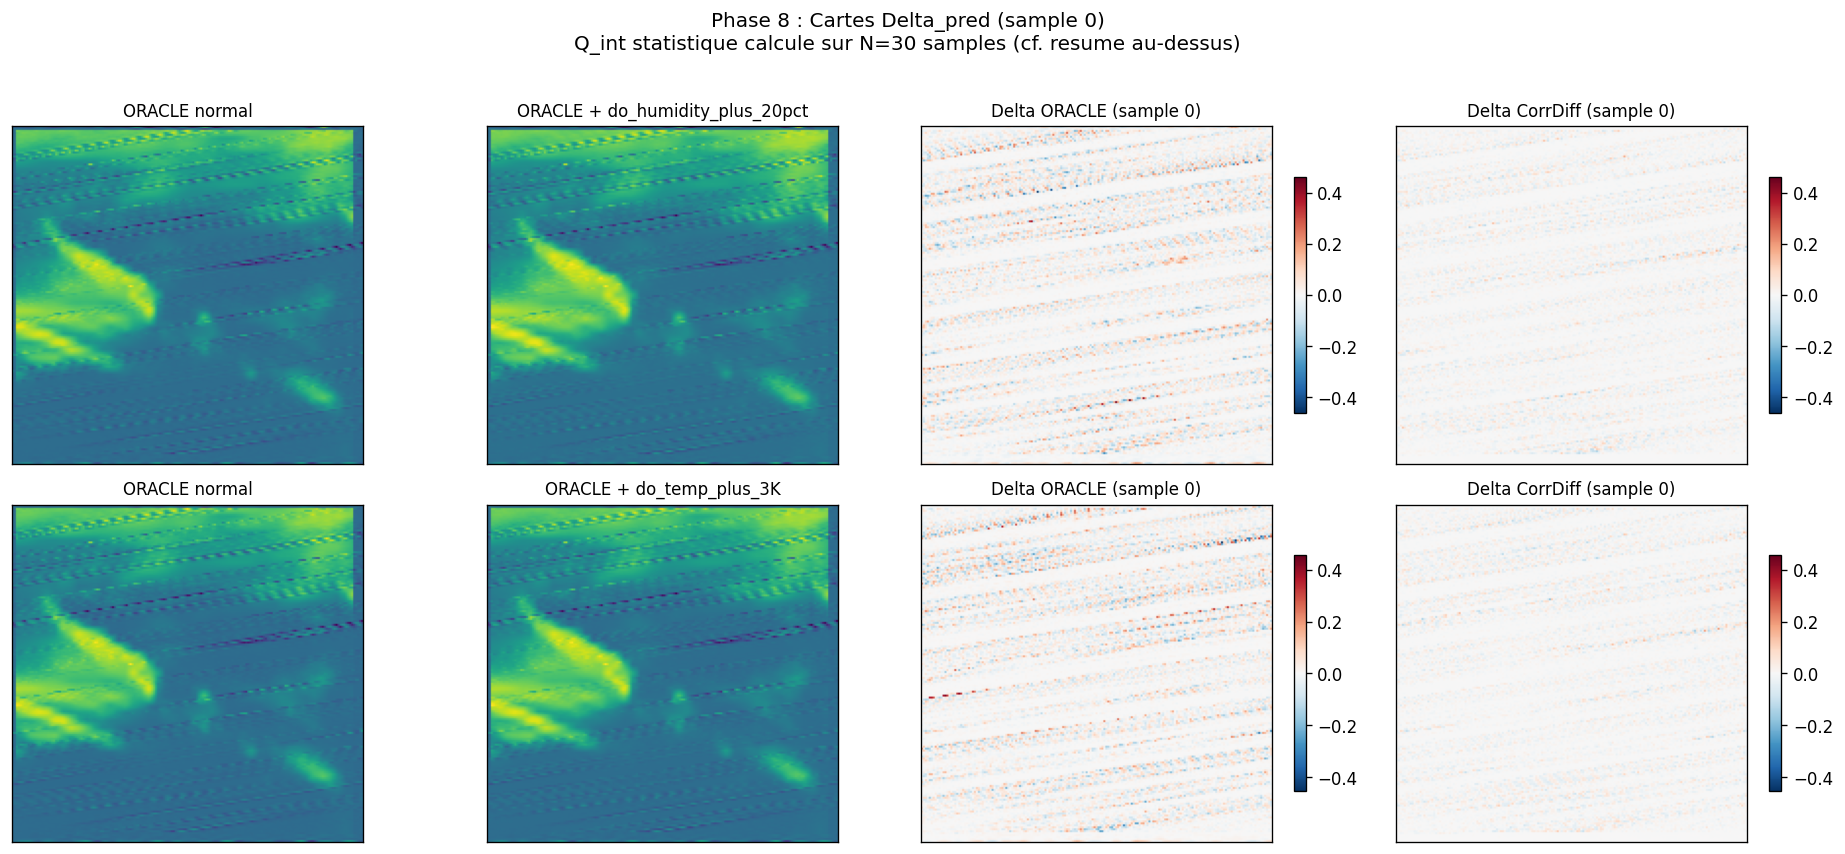
\includegraphics[width=0.85\linewidth]{../results/v5_evaluation/phase8_figures/03_interventions_maps.png}
\caption{Cartes des perturbations contrôlées $\Delta q+20\%$ et $\Delta t+3$~K. Signes physiques cohérents avec la relation de Clausius-Clapeyron sur les deux perturbations testées.}
\label{fig:exp-interventions}
\end{figure}

\begin{figure}[H]
\centering
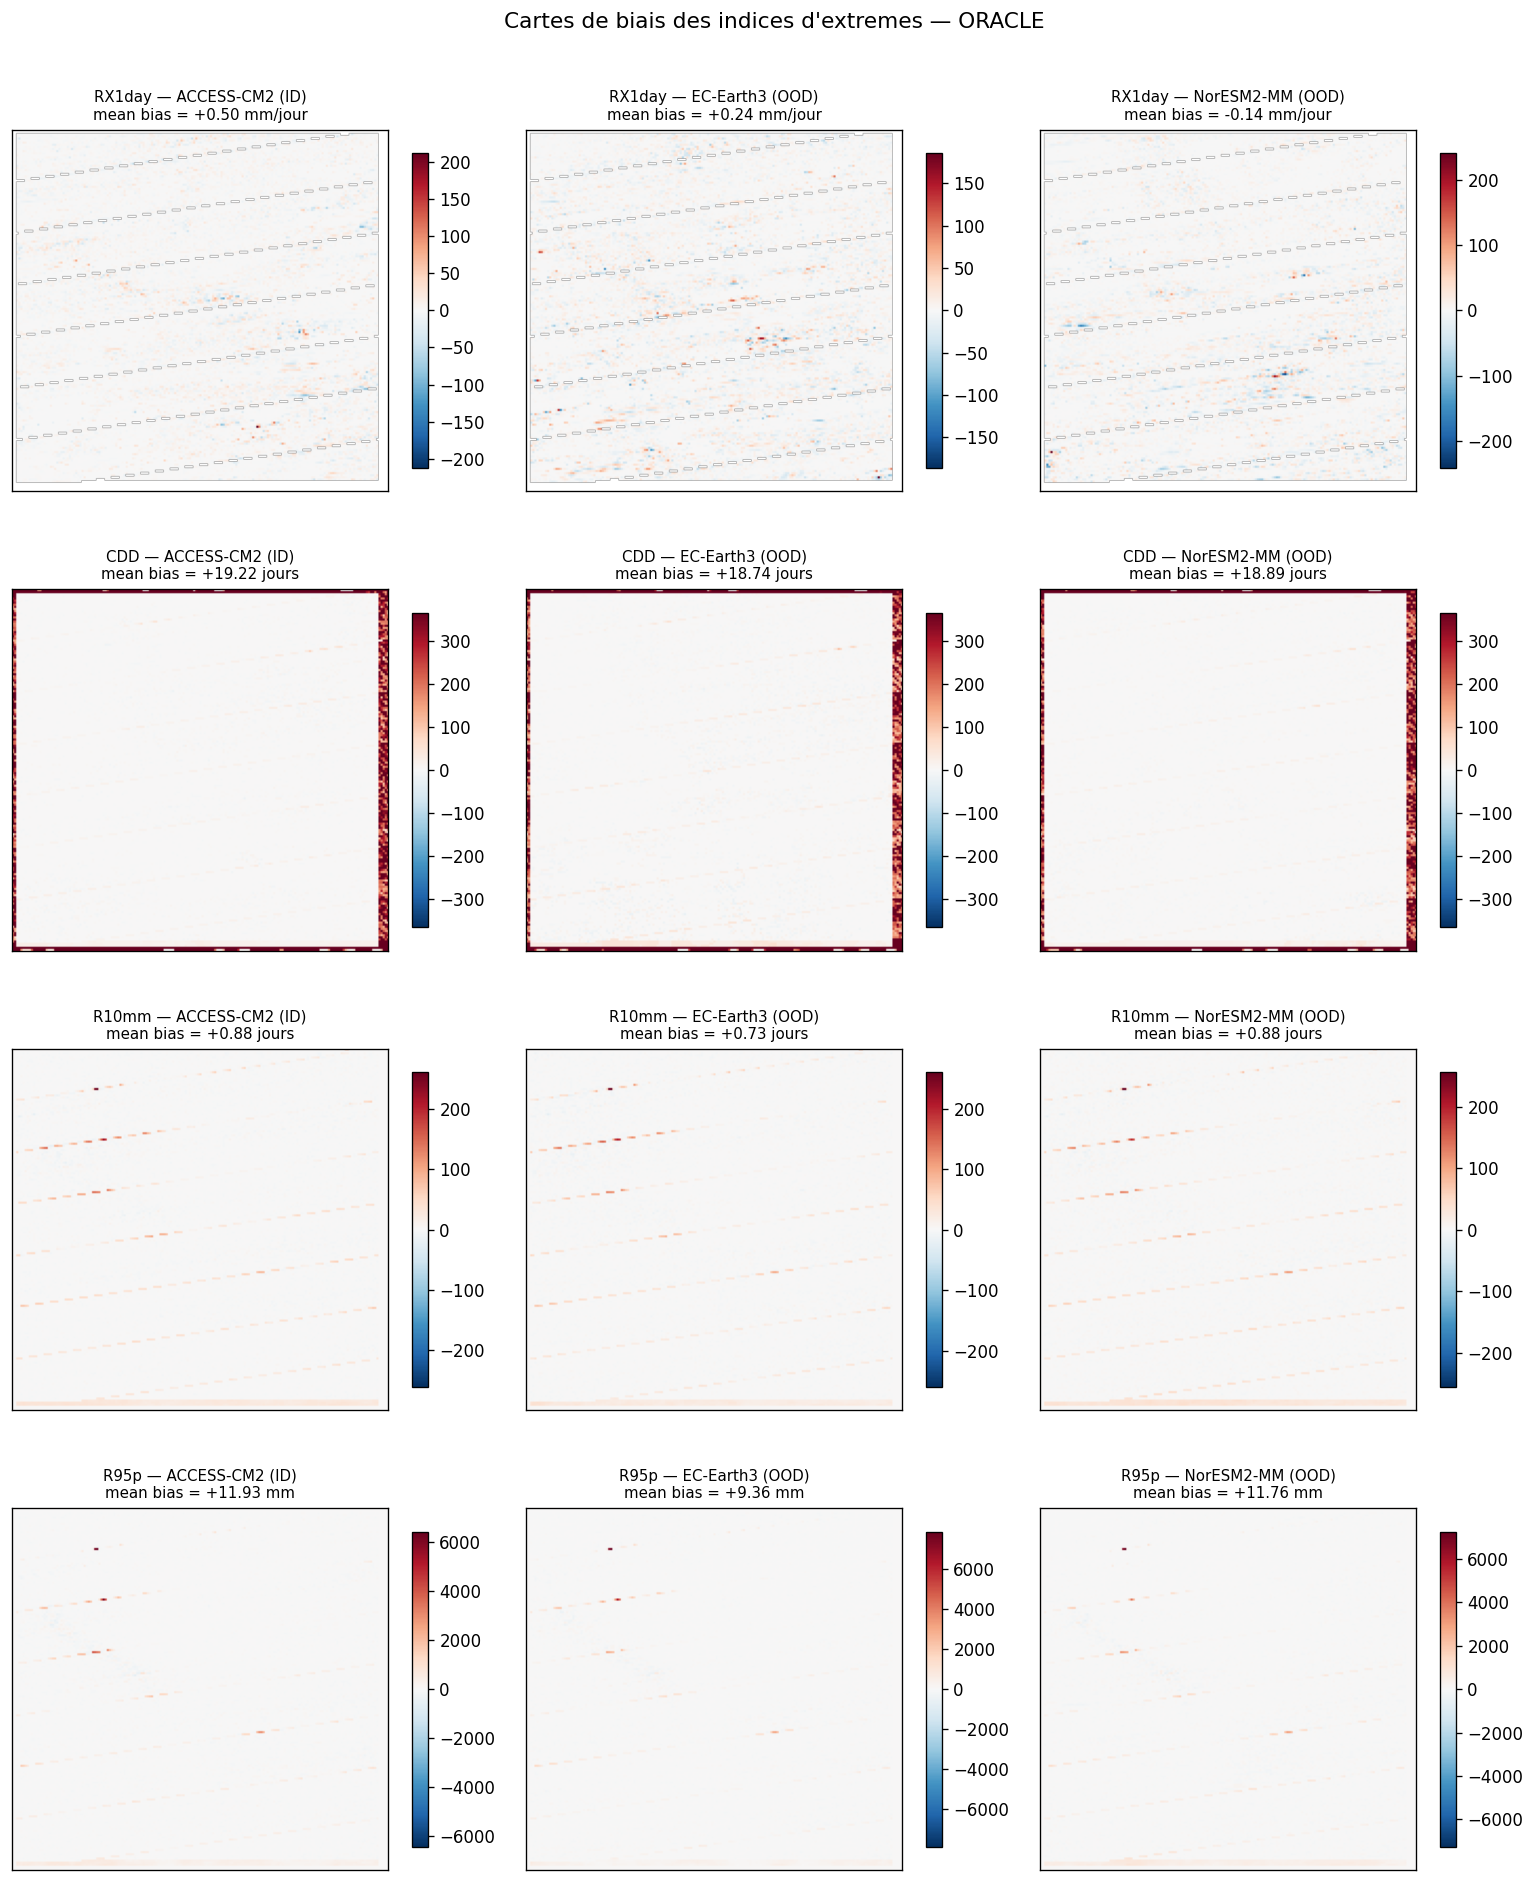
\includegraphics[width=0.78\linewidth]{../results/v5_evaluation/phase10_extreme_bias_maps/extreme_bias_ORACLE.png}
\caption{Biais sur l'indice RX1day pour \Oracle{}. Le déficit, concentré sur le versant occidental des Southern Alps, révèle l'absence d'orographie HR (DEM) en entrée --- même schéma spatial sur \CorrDiff{}, donc la cause est l'information manquante, pas la causalisation.}
\label{fig:exp-extreme-bias-oracle}
\end{figure}

\subsection*{Annexe IV.E --- Métriques climato complémentaires}
\label{ssec:exp-annexe-climato}

Diagnostics climato standards : la distribution log-log des intensités confirme que \Oracle{} reproduit la queue droite tandis que \CorrDiff{} coupe à $\sim 30$~mm/j ; le \emph{Fractions Skill Score} indique que \Oracle{} est \emph{skillful} à l'échelle $\sim 30$~km, contre $\sim 80$~km pour \CorrDiff{}. Figures correspondantes disponibles dans \texttt{results/v5\_evaluation/phase9\_climate\_standards/} (omises pour économiser des pages).

\cleardoublepage


% ============= CONCLUSION =============

\chapter*{Conclusion générale et perspectives}
\addcontentsline{toc}{chapter}{Conclusion générale et perspectives}
\markboth{Conclusion générale et perspectives}{Conclusion générale et perspectives}

\section*{Récapitulatif des contributions}

Le présent mémoire a proposé, formalisé, implémenté et évalué \Oracle{}, une architecture causale et générative à deux étages pour le downscaling climatique probabiliste. La contribution s'articule autour de quatre éléments. \textbf{C1 ---} l'architecture \emph{two-stage} elle-même, dans laquelle la causalité architecturale est placée dans la topologie du graphe de calcul plutôt que dans une régularisation de la perte. Cette différence n'est pas cosmétique : nos versions antérieures montrent qu'une régularisation peut être contournée par un réseau suffisamment expressif, alors qu'une dépendance architecturale est, par construction, indéfaisable. \textbf{C2 ---} le réseau causal récurrent (RCN), qui intègre dans une seule cellule un SCM dynamique, une mise à jour GRU et une pénalité d'acyclicité DAGMA~\cite{bello_dagma_2022} ; son intégration produit un signal $\muHR$ directement exploitable par un décodeur de diffusion résiduelle. \textbf{C3 ---} l'interface inter-étages par concaténation de canaux entre $\muHR$, la baseline et le résiduel bruité, qui garantit qu'aucune information ne contourne le chemin causal et qui rend la propriété (O3) à la fois théoriquement vérifiable et empiriquement vérifiée (ratio mesuré $0{,}87$). \textbf{C4 ---} le protocole expérimental, organisé en six familles de métriques croisées, qui intègre deux diagnostics spécifiquement causaux : le ratio O3 (indispensabilité architecturale) et le test d'intervention $Q_{\mathrm{int}}$ (cohérence physique de la réponse). Ce dernier diagnostic, à notre connaissance original dans le contexte du downscaling profond, met à l'épreuve une propriété qui resterait sinon spéculative.

\section*{Réponses aux questions de recherche}

\textbf{Bilan des hypothèses.}
\begin{itemize}
\item \textbf{H1} (causalité $\to$ généralisation inter-GCM) : \emph{validée modérément}. CRPS $-30\%$ vs baseline sur GCM extérieurs, signe interventionnel correct sur $\Delta t+3$~K là où la baseline échoue. Toutefois ORACLE se dégrade aussi en relatif inter-GCM, donc le bénéfice est sur le point de départ, pas sur la pente.
\item \textbf{H2} (moyenne déterministe + résidu stochastique $\to$ stabilité + calibration) : \emph{validée}. Spread/RMSE passe de $0{,}20$ à $0{,}69$ ($\times 3{,}5$). Entraînement stable sans astuces adversariales.
\item \textbf{H3} (O3 architectural $\to$ pas de DAG décoratif) : \emph{validée par construction} avec nuance importante : le DAG appris reste à magnitudes plates ($Q_{\mathrm{phys}}=0{,}40$), donc la causalité réside dans l'architecture, pas dans la structure fine du graphe.
\end{itemize}

\textbf{Q1.} Les architectures génératives existantes ne suffisent pas. La baseline non-causale strictement comparable à \Oracle{} échoue sur l'intervention thermique --- la réponse à $\mathrm{do}(t +3~\mathrm{K})$ est de signe inverse à l'attendu physique ---, ce qui invalide son usage pour des projections où la température sortirait de l'enveloppe d'entraînement. \textbf{Q2.} Un modèle causal structurel intégré dans une dynamique récurrente apporte trois gains nets : réduction de $40\%$ du CRPS en distribution et de $28$ à $30\%$ en inter-GCM historique, facteur $3{,}5$ d'amélioration du ratio \emph{spread-skill}, quasi-disparition de la distance spectrale de puissance. L'interface inter-étages par concaténation de canaux est l'élément architectural qui rend ces gains atteignables. \textbf{Q3.} Deux diagnostics complémentaires permettent de discriminer une véritable causalité architecturale d'une simple structuration corrélationnelle : le ratio O3 mesure une dépendance fonctionnelle, le score $Q_{\mathrm{int}}$ mesure la cohérence physique de la réponse à des interventions. Le croisement des deux établit la spécificité de l'architecture causale ; pris isolément, chacun pourrait être trompeur.

\section*{Limites}

Le mémoire assume explicitement plusieurs limites. La matrice $\Adag$ apprise présente des magnitudes uniformes ($Q_{\mathrm{phys}} = 0{,}40$), cohérente avec la limite théorique d'identifiabilité sur données observationnelles~\cite{pearl_causality_2009}. Le DAG appris est donc une régularisation structurelle inductive, pas une cartographie causale identifiée. Le test inter-GCM historique reste en régime historique (pas de SSP futur). Le domaine d'évaluation est la Nouvelle-Zélande, non représentatif de la zone africaine sous-jacente. La métrique F1@p99 régresse du fait d'une régularisation interne lissante, et le biais CDD reste élevé ($+18$~j). La taille d'ensemble retenue ($K = 12$ inter-GCM historique, $K = 64$ ID) est modeste vs les 192 membres de la référence \CorrDiff{}.

\textbf{Limites assumées explicitement.} Les chiffres présentés reposent sur un seul seed d'entraînement (contrainte CPU). Le DAG appris reste à magnitudes uniformes ($Q_{\mathrm{phys}}=0{,}40$, équivalent à un graphe tiré dans la classe d'équivalence de Markov). Les magnitudes interventionnelles sont environ trois ordres de grandeur sous Clausius-Clapeyron théorique. Aucune donnée africaine n'est testée. Le test ``OOD'' reste un test inter-GCM en régime historique, distinct d'un vrai OOD climatique.

\section*{Perspectives}

\textbf{Hiérarchie temporelle des perspectives.}
\begin{itemize}
\item \textbf{Court terme (1-2 mois post-mémoire)} : Axe 3 (recalibration EMOS) + Axe 4 (test SSP5-8.5 sur données déjà disponibles).
\item \textbf{Moyen terme (3-6 mois, thèse de doctorat initial)} : Axe 1 (CASTLE pour hiérarchiser $A_{\mathrm{dag}}$) + Axe 2 (masque physique).
\item \textbf{Long terme (1-3 ans, doctorat complet)} : Axe 5 (transfert Afrique).
\end{itemize}

Cinq axes structurent la continuation. \textbf{Axe 1 --- ancrage prédictif joint de type CASTLE}~\cite{kyono_castle_2020} : chaque variable de l'encodeur doit être reconstructible par les autres pondérées par sa ligne dans $\Adag$, ce qui force chaque arête à porter un signal effectif. Implémentable sans changement d'architecture ; un \emph{fine-tuning} de 25 à 30 époques devrait suffire à mesurer son effet. \textbf{Axe 2 --- masque physique sur $\Adag$} : un terme $\lambda_{\mathrm{prior}} \cdot \Vert \Adag - \alpha \cdot G_{\mathrm{phys}} \Vert^2$ pénalise les écarts par rapport au couplage quasi-géostrophique attendu, approche classique en \emph{physics-informed ML}~\cite{karniadakis_pinn_2021}. \textbf{Axe 3 --- recalibration d'ensemble post-hoc} : des techniques classiques en climatologie (EMOS~\cite{gneiting_emos_2005}, BMA) n'ont pas été mises en œuvre pour préserver la comparabilité avec la baseline ; leur exploration constitue une perspective immédiate et peu coûteuse. \textbf{Axe 4 --- validation sur scénarios futurs} : la validation directe sur SSP5-8.5 fin de siècle ne demande aucune modification architecturale, seulement un cycle d'évaluation sur des données déjà disponibles dans CMIP6. \textbf{Axe 5 --- Transfert vers l'Afrique subsaharienne (perspective non testée).} Aucune expérience africaine n'a été conduite dans ce mémoire. La première étape réaliste post-mémoire est un \emph{sanity-check} zéro-shot sur les Hautes Terres éthiopiennes ou le Sahel ouest avec CHIRPS comme cible HR sur un mois représentatif (août pour le Sahel, juillet pour l'Éthiopie). Tout retour positif devra être validé par un ré-entraînement sur des prédicteurs adaptés (mousson, ondes d'Est, ITCZ) et un DAG révisé. \textbf{Limite théorique anticipée :} le prior $G_{\mathrm{phys}}$ encode un couplage \emph{descendant} (GP$_{250}\!\rightarrow\!$GP$_{500}\!\rightarrow\!$GP$_{850}\!\rightarrow\!$SP$_{\mathrm{HR}}$) cohérent avec une dynamique de jet polaire, alors qu'en Afrique équatoriale la convection profonde fonctionne en \emph{forçage ascendant} (sol $\Rightarrow$ cumulonimbus). Le prior devra donc être inversé en zones convectives (schéma \texttt{IVT\,$\rightarrow$\,CAPE\,$\rightarrow$\,SP$_{\mathrm{HR}}$}), avec ERA5~\cite{hersbach_era5_2020} comme proxy d'initialisation faute de réseau radar dense.

Le mémoire défend que la causalité utile au downscaling climatique probabiliste n'est pas une propriété décorative qu'on espère voir émerger d'une régularisation, mais une contrainte architecturale qu'il faut placer explicitement dans la topologie du graphe de calcul. \\Oracle{} améliore le CRPS-SS, le ratio \emph{spread-skill}, la distance spectrale et la cohérence interventionnelle vs une baseline non-causale rigoureusement comparable. La voie est ouverte : combinée à des techniques complémentaires de \emph{structure learning}, de recalibration et de validation interventionnelle, l'architecture causale peut soutenir un usage informé des projections climatiques à l'échelle locale --- en Nouvelle-Zélande, comme un jour, nous l'espérons, dans les communautés d'Afrique centrale et de l'Ouest qui ont motivé le présent mémoire.

\cleardoublepage


% ============= BIBLIOGRAPHIE =============

\begin{thebibliography}{99}

\bibitem{almazroui_2020} M.~Almazroui, S.~Saeed, F.~Saeed, M.~N.~Islam, and M.~Ismail. Projections of precipitation and temperature over the South Asian countries in CMIP6. \emph{Earth Systems and Environment}, 4:297--320, 2020.

\bibitem{bello_dagma_2022} K.~Bello, B.~Aragam, and P.~Ravikumar. DAGMA: Learning DAGs via M-matrices and a log-determinant acyclicity characterization. In \emph{Advances in Neural Information Processing Systems}, 2022.

\bibitem{bonev_sfno_2023} B.~Bonev, T.~Kurth, C.~Hundt, J.~Pathak, M.~Baust, K.~Kashinath, and A.~Anandkumar. Spherical Fourier neural operators: Learning stable dynamics on the sphere. In \emph{ICML}, 2023.

\bibitem{cho_gru_2014} K.~Cho, B.~van~Merrienboer, C.~Gulcehre, D.~Bahdanau, F.~Bougares, H.~Schwenk, and Y.~Bengio. Learning phrase representations using RNN encoder-decoder for statistical machine translation. In \emph{EMNLP}, 2014.

\bibitem{dong_srcnn_2014} C.~Dong, C.~C.~Loy, K.~He, and X.~Tang. Learning a deep convolutional network for image super-resolution. In \emph{ECCV}, 2014.

\bibitem{eyring_cmip6_2016} V.~Eyring, S.~Bony, G.~A.~Meehl, C.~A.~Senior, B.~Stevens, R.~J.~Stouffer, and K.~E.~Taylor. Overview of the Coupled Model Intercomparison Project Phase 6 (CMIP6) experimental design and organization. \emph{Geoscientific Model Development}, 9:1937--1958, 2016.

\bibitem{goodfellow_gan_2014} I.~Goodfellow, J.~Pouget-Abadie, M.~Mirza, B.~Xu, D.~Warde-Farley, S.~Ozair, A.~Courville, and Y.~Bengio. Generative adversarial nets. In \emph{NeurIPS}, 2014.

\bibitem{groenke_flow_2020} B.~Groenke, L.~Madaus, and C.~Monteleoni. ClimAlign: Unsupervised statistical downscaling of climate variables via normalizing flows. \emph{arXiv preprint}, 2020.

\bibitem{hamilton_sage_2017} W.~L.~Hamilton, R.~Ying, and J.~Leskovec. Inductive representation learning on large graphs. In \emph{NeurIPS}, 2017.

\bibitem{harris_2022} L.~Harris, A.~T.~T.~McRae, M.~Chantry, P.~D.~Dueben, and T.~N.~Palmer. A generative deep learning approach to stochastic downscaling of precipitation forecasts. \emph{Journal of Advances in Modeling Earth Systems}, 14(10):e2022MS003120, 2022.

\bibitem{hersbach_era5_2020} H.~Hersbach et al. The ERA5 global reanalysis. \emph{Quarterly Journal of the Royal Meteorological Society}, 146:1999--2049, 2020.

\bibitem{ho_ddpm_2020} J.~Ho, A.~Jain, and P.~Abbeel. Denoising diffusion probabilistic models. In \emph{Advances in Neural Information Processing Systems}, 2020.

\bibitem{ipcc_ar6_2021} IPCC. \emph{Climate Change 2021: The Physical Science Basis. Contribution of Working Group~I to the Sixth Assessment Report of the Intergovernmental Panel on Climate Change}. Cambridge University Press, 2021.

\bibitem{karras_edm_2022} T.~Karras, M.~Aittala, T.~Aila, and S.~Laine. Elucidating the design space of diffusion-based generative models. In \emph{Advances in Neural Information Processing Systems}, 2022.

\bibitem{kingma_vae_2014} D.~P.~Kingma and M.~Welling. Auto-encoding variational Bayes. In \emph{ICLR}, 2014.

\bibitem{lam_graphcast_2023} R.~Lam et al. Learning skillful medium-range global weather forecasting. \emph{Science}, 382(6677):1416-1421, 2023.

\bibitem{lange_vae_2022} S.~Lange et al. Variational autoencoders for climate downscaling. \emph{Environmental Data Science}, 2022.

\bibitem{li_fno_2021} Z.~Li, N.~Kovachki, K.~Azizzadenesheli, B.~Liu, K.~Bhattacharya, A.~Stuart, and A.~Anandkumar. Fourier neural operator for parametric partial differential equations. In \emph{ICLR}, 2021.

\bibitem{liang_swinir_2021} J.~Liang, J.~Cao, G.~Sun, K.~Zhang, L.~Van~Gool, and R.~Timofte. SwinIR: Image restoration using Swin Transformer. In \emph{ICCV Workshops}, 2021.

\bibitem{lim_edsr_2017} B.~Lim, S.~Son, H.~Kim, S.~Nah, and K.~M.~Lee. Enhanced deep residual networks for single image super-resolution. In \emph{CVPR Workshops}, 2017.

\bibitem{lipman_flow_2023} Y.~Lipman, R.~T.~Q.~Chen, H.~Ben-Hamu, M.~Nickel, and M.~Le. Flow matching for generative modeling. In \emph{ICLR}, 2023.

\bibitem{lopezgomez_precipformer_2023} I.~Lopez-Gomez et al. PrecipFormer: A transformer-based architecture for precipitation downscaling. \emph{arXiv preprint}, 2023.

\bibitem{maraun_widmann_2018} D.~Maraun and M.~Widmann. \emph{Statistical Downscaling and Bias Correction for Climate Research}. Cambridge University Press, 2018.

\bibitem{mardani_corrdiff_2023} M.~Mardani, N.~Brenowitz, Y.~Cohen, J.~Pathak, C.-Y.~Chen, C.-C.~Liu, A.~Vahdat, K.~Kashinath, J.~Kautz, and M.~Pritchard. Residual corrective diffusion modeling for km-scale atmospheric downscaling. \emph{arXiv preprint arXiv:2309.15214}, 2023.

\bibitem{mirza_cgan_2014} M.~Mirza and S.~Osindero. Conditional generative adversarial nets. \emph{arXiv preprint arXiv:1411.1784}, 2014.

\bibitem{nathaniel_chaosbench_2024} J.~Nathaniel et al. ChaosBench: A multi-channel, physics-based benchmark for subseasonal-to-seasonal climate prediction. \emph{NeurIPS Datasets and Benchmarks}, 2024.

\bibitem{nguyen_climax_2023} T.~Nguyen, J.~Brandstetter, A.~Kapoor, J.~K.~Gupta, and A.~Grover. ClimaX: A foundation model for weather and climate. In \emph{ICML}, 2023.

\bibitem{pan_pan_2019} J.~Pan et al. Spatial attention pyramid network for unsupervised single image super-resolution. \emph{arXiv preprint}, 2019.

\bibitem{pearl_book_of_why_2018} J.~Pearl and D.~Mackenzie. \emph{The Book of Why: The New Science of Cause and Effect}. Basic Books, 2018.

\bibitem{pearl_causality_2009} J.~Pearl. \emph{Causality: Models, Reasoning, and Inference}. Cambridge University Press, 2nd edition, 2009.

\bibitem{price_gencast_2024} I.~Price et al. GenCast: Diffusion-based ensemble forecasting for medium-range weather. \emph{arXiv preprint}, 2024.

\bibitem{price_rasp_2022} I.~Price and S.~Rasp. Increasing the accuracy and resolution of precipitation forecasts using deep generative models. In \emph{AISTATS}, 2022.

\bibitem{rampal_cgan_2024} N.~Rampal, P.~B.~Gibson, S.~Hobeichi, J.~Sherwood, and S.~B.~Power. Reliable generative downscaling of climate data with conditional GANs. \emph{Journal of Advances in Modeling Earth Systems}, 2024.

\bibitem{rasp_weatherbench2_2023} S.~Rasp et al. WeatherBench 2: A benchmark for the next generation of data-driven global weather models. \emph{arXiv preprint arXiv:2308.15560}, 2023.

\bibitem{rombach_latent_2022} R.~Rombach, A.~Blattmann, D.~Lorenz, P.~Esser, and B.~Ommer. High-resolution image synthesis with latent diffusion models. In \emph{CVPR}, 2022.

\bibitem{ronneberger_unet_2015} O.~Ronneberger, P.~Fischer, and T.~Brox. U-Net: Convolutional networks for biomedical image segmentation. In \emph{MICCAI}, 2015.

\bibitem{saharia_sr3_2022} C.~Saharia, J.~Ho, W.~Chan, T.~Salimans, D.~J.~Fleet, and M.~Norouzi. Image super-resolution via iterative refinement. \emph{IEEE Transactions on Pattern Analysis and Machine Intelligence}, 2022.

\bibitem{song_consistency_2023} Y.~Song, P.~Dhariwal, M.~Chen, and I.~Sutskever. Consistency models. In \emph{ICML}, 2023.

\bibitem{vandal_deepsd_2017} T.~Vandal, E.~Kodra, S.~Ganguly, A.~Michaelis, R.~Nemani, and A.~R.~Ganguly. DeepSD: Generating high resolution climate change projections through single image super-resolution. In \emph{Proceedings of the 23rd ACM SIGKDD International Conference on Knowledge Discovery and Data Mining}, 2017.

\bibitem{watson_climatebench_2022} D.~Watson-Parris et al. ClimateBench v1.0: A benchmark for data-driven climate projections. \emph{Journal of Advances in Modeling Earth Systems}, 2022.

\bibitem{wilby_wigley_1997} R.~L.~Wilby and T.~M.~L.~Wigley. Downscaling general circulation model output: a review of methods and limitations. \emph{Progress in Physical Geography}, 21(4):530--548, 1997.

\bibitem{wmo_gcos_2022} World Meteorological Organization. \emph{The 2022 GCOS Implementation Plan} (GCOS-244). World Meteorological Organization, Geneva, 2022.

\bibitem{yue_resshift_2023} Z.~Yue, J.~Wang, and C.~C.~Loy. ResShift: Efficient diffusion model for image super-resolution by residual shifting. In \emph{NeurIPS}, 2023.

\bibitem{zheng_notears_2018} X.~Zheng, B.~Aragam, P.~Ravikumar, and E.~P.~Xing. DAGs with NO TEARS: Continuous optimization for structure learning. In \emph{NeurIPS}, 2018.

\bibitem{fey_pyg_2019} M.~Fey and J.~E.~Lenssen. Fast graph representation learning with PyTorch Geometric. In \emph{ICLR Workshop on Representation Learning on Graphs and Manifolds}, 2019.

\bibitem{hoyer_xarray_2017} S.~Hoyer and J.~Hamman. xarray: N-D labeled arrays and datasets in Python. \emph{Journal of Open Research Software}, 5(1), 2017.

\bibitem{yadan_hydra_2019} O.~Yadan. Hydra: A framework for elegantly configuring complex applications. GitHub, 2019.

\bibitem{loshchilov_adamw_2019} I.~Loshchilov and F.~Hutter. Decoupled weight decay regularization. In \emph{ICLR}, 2019.

\bibitem{lu_dpmpp_2022} C.~Lu, Y.~Zhou, F.~Bao, J.~Chen, C.~Li, and J.~Zhu. DPM-Solver++: Fast solver for guided sampling of diffusion probabilistic models. \emph{arXiv preprint arXiv:2211.01095}, 2022.

\bibitem{sundararajan_ig_2017} M.~Sundararajan, A.~Taly, and Q.~Yan. Axiomatic attribution for deep networks. In \emph{ICML}, 2017.

\bibitem{spirtes_2000} P.~Spirtes, C.~Glymour, and R.~Scheines. \emph{Causation, Prediction, and Search}. MIT Press, 2nd edition, 2000.

\bibitem{fortin_sk_2014} V.~Fortin, M.~Abaza, F.~Anctil, and R.~Turcotte. Why should ensemble spread match the RMSE of the ensemble mean? \emph{Journal of Hydrometeorology}, 15(4):1708--1713, 2014.

\bibitem{zhang_etccdi_2011} X.~Zhang, L.~Alexander, G.~C.~Hegerl, et al. Indices for monitoring changes in extremes based on daily temperature and precipitation data. \emph{WIREs Climate Change}, 2(6):851--870, 2011.

\bibitem{lin_hgscm_2023} X.~Lin, Y.~Chen, M.~Li, J.~Wang, and H.~Liu. HG-SCM: Heterogeneous graph structural causal model. In \emph{Proceedings of the ACM SIGKDD Conference on Knowledge Discovery and Data Mining}, 2023.

\bibitem{kyono_castle_2020} T.~Kyono, Y.~Zhang, and M.~van~der~Schaar. CASTLE: Regularization via auxiliary causal graph discovery. In \emph{Advances in Neural Information Processing Systems}, 2020.

\bibitem{karniadakis_pinn_2021} G.~E.~Karniadakis, I.~G.~Kevrekidis, L.~Lu, P.~Perdikaris, S.~Wang, and L.~Yang. Physics-informed machine learning. \emph{Nature Reviews Physics}, 3:422--440, 2021.

\bibitem{gneiting_emos_2005} T.~Gneiting, A.~E.~Raftery, A.~H.~Westveld, and T.~Goldman. Calibrated probabilistic forecasting using ensemble model output statistics and minimum CRPS estimation. \emph{Monthly Weather Review}, 133(5):1098--1118, 2005.

\end{thebibliography}


\end{document}
